\documentclass[11pt,a4paper]{book}

% -----------------------
% Pacchetti base
% -----------------------
\usepackage[utf8]{inputenc}
\usepackage[T1]{fontenc}
\usepackage[italian]{babel}
\usepackage{amsmath,amssymb}
\usepackage{graphicx}
\usepackage{hyperref}
\usepackage{geometry}
\usepackage{fancyhdr}
\usepackage{titlesec}
\usepackage{parskip}
\usepackage{color}
\usepackage{siunitx}
\usepackage{physics}

% -----------------------
% Layout
% -----------------------
\geometry{margin=2.5cm}
\pagestyle{fancy}
\fancyhf{}
\fancyfoot[C]{\thepage}
\fancyhead[L]{\leftmark}
\renewcommand{\headrulewidth}{0.4pt}

% -----------------------
% Colori e link
% -----------------------
\hypersetup{
    colorlinks=true,
    linkcolor=blue,
    citecolor=blue,
    urlcolor=blue,
    pdftitle={Appunti di Fisica dei Materiali per la Fotonica}
}

% -----------------------
% Stile titoli capitoli
% -----------------------
\titleformat{\chapter}[display]
  {\normalfont\huge\bfseries}
  {\filleft\Huge\thechapter}
  {1ex}
  {\titlerule\vspace{1ex}\filright}
  [\vspace{1ex}\titlerule]

% -----------------------
% Copertina
% -----------------------
\begin{document}
\begin{titlepage}
    \centering
    \vspace*{2cm}
    
    {\scshape\LARGE Università di Pisa \par}
    \vspace{1.5cm}
    {\Huge\bfseries Notes on \\[0.5cm]
    Physics of Materials for Photonics\par}
    \vspace{2cm}
    {\Large\itshape Course taught by Prof. Riccardo Farchioni\par}
    \vfill
    {\large Notes written by Jacopo Martellotto\par}
    \vspace{0.5cm}
    {\large \today\par}
\end{titlepage}
% -----------------------
% Indice
% -----------------------
\tableofcontents
\newpage

% -----------------------
% Capitoli inclusi
% -----------------------
\chapter{Introduzione}

\section{Cosa studia la fotonica}
La fotonica si occupa dello studio della luce e della sua interazione con i materiali...

\section{Applicazioni}
Tra le principali applicazioni troviamo:
\begin{itemize}
    \item Comunicazioni ottiche
    \item Sensori fotonici
    \item Laser e spettroscopia
\end{itemize}

\chapter{Semiconductor Bandstructure}

\section{Introduction}
The behavior of electrons in semiconductors is governed by the solutions to the Schrödinger equation tailored to the crystal environment. These solutions yield the electronic bandstructure, which characterizes the allowed energy states for electrons in the material. Determining the electronic spectrum is, however, a highly complex task. In solids, the presence of a vast number of atoms arranged closely together generates a complicated potential energy landscape for electrons. Furthermore, electron–electron interactions and dynamic lattice vibrations (phonons) introduce additional complexity through time-dependent variations in the potential.
To make the problem tractable, the effects of atomic vibrations and electron–electron scattering are initially excluded and later incorporated using perturbation theory. These effects primarily contribute to the scattering of electrons between different quantum states.
The analysis of bandstructure becomes significantly more manageable in crystalline solids. In such systems, the electrons move in a spatially periodic potential due to the regular arrangement of atoms. This periodicity leads to solutions that obey Bloch’s theorem, which will be addressed in the following section.
Realistic methods for computing the bandstructure of semiconductors generally fall into two broad categories:
\begin{enumerate}
	\item Approaches that capture the full conduction and valence band profiles.
	\item Approaches that focus specifically on the bandstructure near the band edges.
\end{enumerate}

\section{Block Theorem and Crystal Momentum}
To analyze the electronic characteristics of a material, it is essential to determine the electron wavefunctions and their corresponding energies within a solid. In this context, we focus solely on crystalline materials. The behavior of electrons in a periodic solid is governed by the Schrödinger equation:
\begin{equation*}
	\left[-\frac{\hbar^2}{2m} \nabla^2 + U(\mathbf{r})\right] \psi(\mathbf{r}) = E \psi(\mathbf{r})
\end{equation*}
Here, \( U(\mathbf{r}) \) represents the potential energy experienced by the electrons. Owing to the periodic structure of the crystal, this potential exhibits the same periodicity \( \mathbf{R} \) as the lattice:
\begin{equation*}
	U(\mathbf{r}) = U(\mathbf{r} + \mathbf{R})
\end{equation*}
In the case where the background potential is absent, the electron wavefunction within a volume \( V \) takes the form \( \psi(\mathbf{r}) = \frac{1}{\sqrt{V}} e^{i\mathbf{k} \cdot \mathbf{r}} \), and the corresponding momentum and energy of the electron are given by:
\begin{equation*}
	\mathbf{p} = \hbar \mathbf{k}, \quad E = \frac{\hbar^2 k^2}{2m}
\end{equation*}
This wavefunction is delocalized over the entire sample, implying that the probability density \( \psi^* \psi \) is uniform throughout space.

When considering a periodic crystal, it is expected that the electron probability distribution remains identical in each unit cell, since all cells are structurally the same. If the potential were disordered, this uniformity would not hold. Given a lattice translation vector \( \mathbf{R} \), we require:
\begin{equation*}
	|\psi(\mathbf{r})|^2 = |\psi(\mathbf{r} + \mathbf{R})|^2
\end{equation*}
This condition ensures that one cannot distinguish between different unit cells based on electronic probability density. It is important to note that while the probability is periodic, the wavefunction itself need not be. The appropriate form of the wavefunction in a periodic potential is described by Bloch’s theorem. According to this theorem, the eigenfunctions of the Schrödinger equation in a periodic lattice are of the form:
\begin{equation*}
	\psi_{\mathbf{k}}(\mathbf{r}) = u_{\mathbf{k}}(\mathbf{r}) e^{i\mathbf{k} \cdot \mathbf{r}}
\end{equation*}
where \( u_{\mathbf{k}}(\mathbf{r}) \) is a function that shares the periodicity of the crystal:
\begin{equation*}
	u_{\mathbf{k}}(\mathbf{r}) = u_{\mathbf{k}}(\mathbf{r} + \mathbf{R})
\end{equation*}
\begin{center}
	\begin{minipage}{0.6\textwidth}
		\centering
		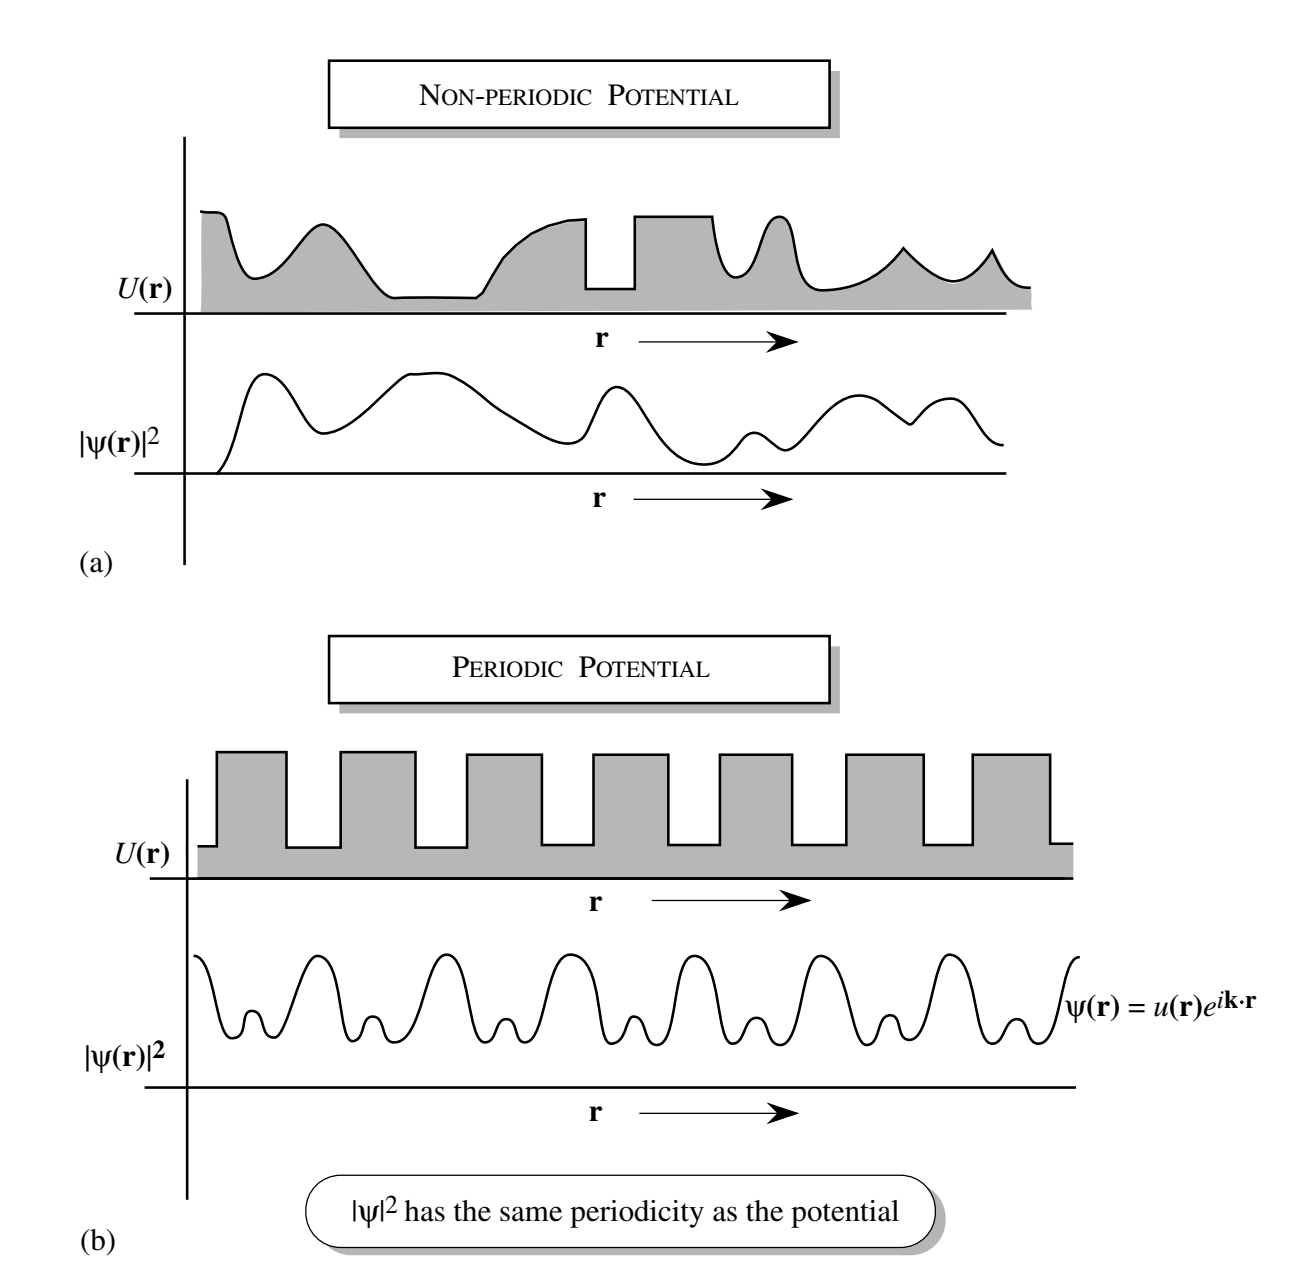
\includegraphics[width=\textwidth]{img/periodic_potential.png}
		\\[0.5em]
		\refstepcounter{figure}
		\textbf{Figure~\thefigure.} (a) Example of an electronic wavefunction in a disordered material. (b) In a periodic potential, \( |\psi|^2 \) shares the same periodicity, as required by Bloch's theorem.
		\label{fig:periodic_potential}
	\end{minipage}
\end{center}
This implies that the full wavefunction transforms under lattice translations as:
\begin{equation*}
	\psi_{\mathbf{k}}(\mathbf{r} + \mathbf{R}) = u_{\mathbf{k}}(\mathbf{r} + \mathbf{R}) e^{i\mathbf{k} \cdot (\mathbf{r} + \mathbf{R})} = u_{\mathbf{k}}(\mathbf{r}) e^{i\mathbf{k} \cdot \mathbf{r}} e^{i\mathbf{k} \cdot \mathbf{R}} = \psi_{\mathbf{k}}(\mathbf{r}) e^{i\mathbf{k} \cdot \mathbf{R}}
\end{equation*}
The vector \( \mathbf{k} \), known as the wavevector or \( \mathbf{k} \)-vector, is fundamental in describing the electronic properties of crystalline solids.

\subsection{Significance of the k-Vector}
One of the key consequences of Bloch's theorem is that, in a perfectly periodic potential provided by the crystal lattice, electrons can propagate through the material without experiencing scattering. In such a scenario, the electron wavefunction, which resembles \( \sim e^{i\mathbf{k} \cdot \mathbf{r}} \), describes an extended state that spans the entire crystal.
To understand how electrons behave under external influences, we seek to derive an equation of motion that captures their response to external forces. Let \( \mathbf{F}_{\text{ext}} \) denote an external force acting on the electron, and \( \mathbf{F}_{\text{int}} \) represent the internal force arising from the atomic lattice. Newton’s second law can then be expressed as:
\begin{equation*}
	\frac{d\mathbf{p}}{dt} = \mathbf{F}_{\text{ext}} + \mathbf{F}_{\text{int}}
\end{equation*}
\noindent However, this form is not particularly useful, as it involves the internal forces, which are typically complex to evaluate. To describe the electron's motion more effectively, we need an equation that depends solely on the external forces. We now outline a simplified derivation of such an expression, which also helps clarify the physical interpretation of the wavevector \( \mathbf{k} \) introduced in Bloch’s theorem.
Starting from the time-dependent Schrödinger equation, the general solution for electrons in a periodic potential can be written as:
\begin{equation*}
	\psi(\mathbf{r}, t) = u_{\mathbf{k}}(\mathbf{r}) e^{i(\mathbf{k} \cdot \mathbf{r} - \omega t)}
\end{equation*}
\noindent where the energy of the electron is connected to the angular frequency \( \omega \) by the relation:
\begin{equation*}
	E = \hbar \omega
\end{equation*}
\noindent The Bloch function thus corresponds to a plane wave that extends throughout the crystalline solid. To describe a spatially localized electron, we consider a wavepacket composed of Bloch states centered around a specific wavevector \( \mathbf{k} \). The group velocity of this wavepacket is given by:
\begin{equation*}
	\mathbf{v}_g = \frac{d\omega}{d\mathbf{k}} = \frac{1}{\hbar} \frac{dE}{d\mathbf{k}} = \frac{1}{\hbar} \nabla_{\mathbf{k}} E(\mathbf{k})
\end{equation*}

In the presence of an electric field \( \mathbf{F} \), the energy gained by the electron over a short time interval \( \delta t \) is:
\begin{equation*}
	\delta E = -e \mathbf{F} \cdot \mathbf{v}_g \, \delta t
\end{equation*}
\noindent More generally, the change in energy can be expressed as:
\begin{equation*}
	\delta E = \frac{dE}{d\mathbf{k}} \cdot \delta \mathbf{k} = \hbar \mathbf{v}_g \cdot \delta \mathbf{k}
\end{equation*}
\noindent Equating the two expressions for \( \delta E \), we obtain:
\begin{equation*}
	\delta \mathbf{k} = -\frac{e \mathbf{F}}{\hbar} \delta t
\end{equation*}
\noindent which leads to the equation of motion for the wavevector:
\begin{equation*}
	\hbar \frac{d\mathbf{k}}{dt} = -e \mathbf{F}
\end{equation*}
\noindent Since \( -e\mathbf{F} \) is the force acting on the electron, this can be generalized to:
\begin{equation*}
	\hbar \frac{d\mathbf{k}}{dt} = \mathbf{F}_{\text{ext}}
\end{equation*}
\noindent This result mirrors Newton’s second law:
\begin{equation*}
	\frac{d\mathbf{p}}{dt} = \mathbf{F}_{\text{ext}}
\end{equation*}
\noindent provided we identify \( \hbar d\mathbf{k} \) with the momentum of the electron inside the crystal. While \( \hbar d\mathbf{k} \) behaves as the momentum in response to external forces, it is not the true mechanical momentum since it incorporates the effects of the internal periodic potential. Instead, \( \hbar \mathbf{k} \) is referred to as the \textit{crystal momentum}.

\section{Metals, Insulators, and Semiconductors}
From atomic physics, it is known that bound electrons occupy discrete energy levels, separated by regions where no states exist. In solids, these discrete levels broaden into continuous energy bands, with forbidden gaps—bandgaps—separating them. Once the electronic band structure is known, a key question arises: which of the available states are occupied by electrons, and which remain empty?
Two important cases emerge regarding electron occupation: in one scenario, an energy band is fully occupied at 0~K, while the next higher band is separated by an energy gap \( E_g \) and remains completely unoccupied. In the second case, the highest energy band that contains electrons is only partially filled.
At this stage, a critical concept must be introduced. When an energy band is completely filled, the electrons within it cannot contribute to electrical conduction. This is a direct consequence of the Pauli exclusion principle: since electrons are fermions, they can only transition into unoccupied states. In a filled band, all such states are already occupied, leading to a cancellation of net motion—electrons moving in opposite directions balance each other. As a result, materials with fully filled bands and an energy gap above them exhibit, in principle, infinite resistivity and are classified as insulators or semiconductors.
In contrast, if the highest occupied band is only partially filled, available empty states exist within the same band. This allows electrons to accelerate under an external field, enabling electrical conduction. Such materials exhibit low resistivity and are termed metals.
\begin{center}
	\begin{minipage}{0.6\textwidth}
		\centering
		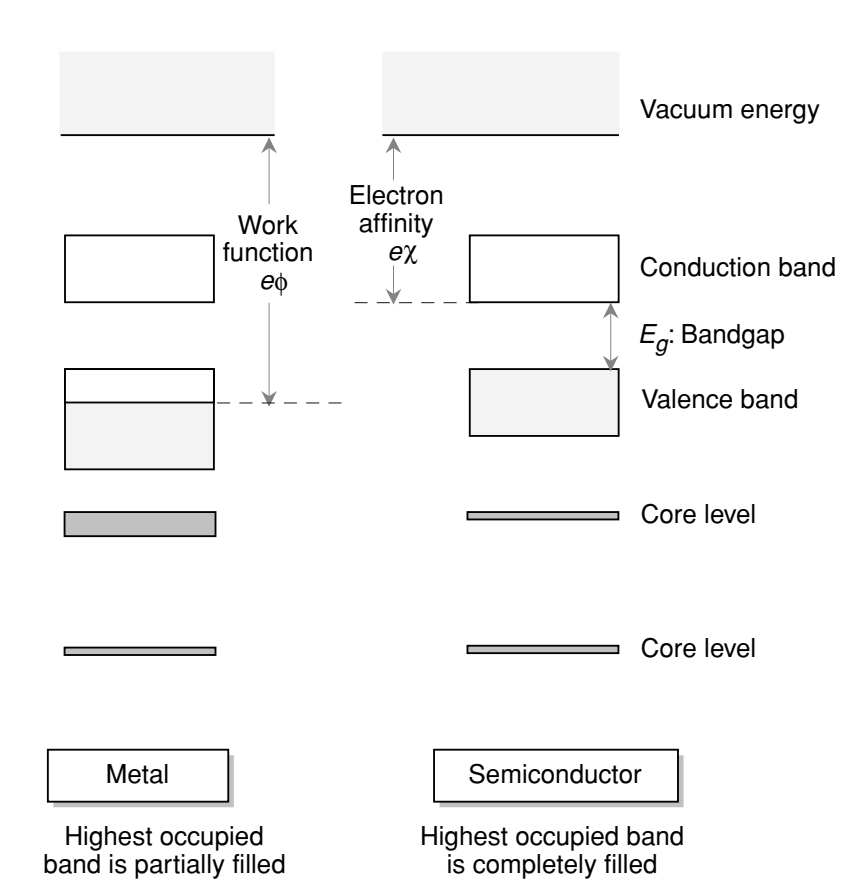
\includegraphics[width=\textwidth]{img/metalsVSsemiconductors.png}
		\\[0.5em]
		\refstepcounter{figure}
		\textbf{Figure~\thefigure.} Band occupation at 0~K for a metal and a semiconductor. In metals, the top band is partially filled. In semiconductors, the valence band is full and separated from the empty conduction band by the bandgap \( E_g \). Work function and electron affinity are indicated.
		\label{fig:metalsVSsemiconductors}
	\end{minipage}
\end{center}
The band that is fully occupied by electrons at absolute zero in semiconductors is known as the \textit{valence band}, whereas the higher energy band that remains empty at 0~K is referred to as the \textit{conduction band}. In metals, the energy difference between the vacuum level and the highest occupied electronic state is termed the \textit{work function}. For semiconductors, the energy separating the vacuum level from the bottom of the conduction band is called the \textit{electron affinity}.
Metals are characterized by extremely high electrical conductivity, resulting from the large number of electrons available for conduction. However, this abundance of charge carriers also makes it difficult to significantly modify their conductivity. Semiconductors, in contrast, exhibit zero conductivity at 0~K and relatively low conductivity at finite temperatures. Importantly, their conductivity can be altered dramatically—by several orders of magnitude—which is the foundation of their utility in active electronic components.
As previously discussed, semiconductors are defined as materials in which the valence band is completely filled and the conduction band completely empty at 0~K. When the temperature is raised above absolute zero, some electrons gain enough thermal energy to transition from the valence band into the conduction band. This results in the creation of empty states (holes) in the valence band and free electrons in the conduction band.
When electrons are thermally excited into the conduction band, the valence band is left with some unoccupied states. Consider the situation illustrated in the scheme below, where an electron with wavevector \( \mathbf{k}_e \) is missing from the valence band. In a completely filled valence band, the total sum over all electron wavevectors is zero:

\begin{equation*}
	\sum_i \mathbf{k}_i = \sum_{\mathbf{k}_e} \mathbf{k}_e + \sum_{-\mathbf{k}_e} (-\mathbf{k}_e) = 0
\end{equation*}
\noindent
This simply reflects the fact that for every occupied positive wavevector state, there exists a corresponding occupied state with a negative wavevector.

Now, when an electron is missing from a particular state \( \mathbf{k}_e \), the net wavevector of the system becomes:
\begin{equation*}
	\mathbf{k}_h = -\mathbf{k}_e
\end{equation*}
\noindent
This unoccupied state is referred to as a \textit{hole}, and the wavevector \( -\mathbf{k}_e \) is attributed to it. Although the missing electron originated from the state \( \mathbf{k}_e \), the hole is described as having wavevector \( \mathbf{k}_h = -\mathbf{k}_e \), as illustrated. The hole's position corresponds to where the electron would have been.

It is important to emphasize that a hole represents the absence of an electron in the valence band. When the valence band is completely filled, it cannot contribute to electrical conduction. However, once an electron is removed, current can flow. Under the application of an electric field, electrons drift in the direction opposite to the field, which effectively causes the unoccupied (hole) state to move in the direction of the field. Thus, the hole behaves like a positively charged particle.

\begin{center}
	\begin{minipage}{0.7\textwidth}
		\centering
		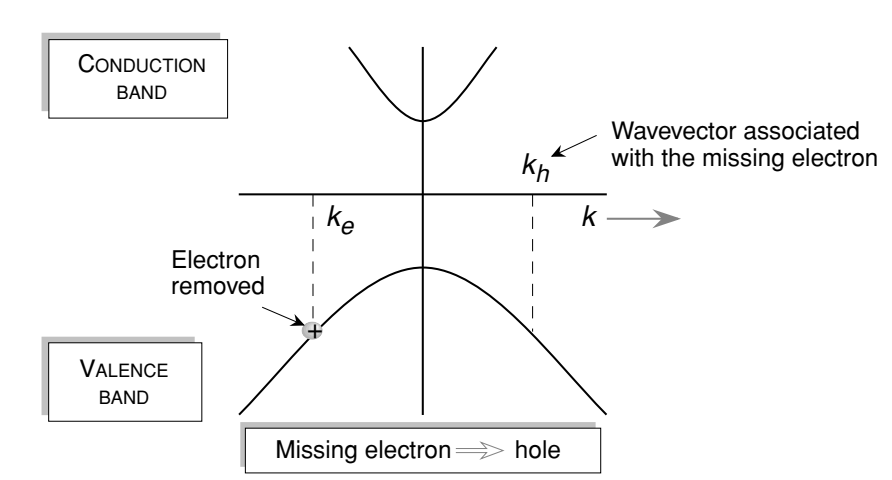
\includegraphics[width=\textwidth]{img/missingelectron.png}
		\\[0.5em]
		\refstepcounter{figure}
		\textbf{Figure~\thefigure.} Illustration of a the wavector of the missng electron $\mathbf{k}_e$ and the corresponding hole wavevector $-\mathbf{k}_e$.
		\label{fig:missingelectron}
	\end{minipage}
\end{center}

The response of the hole to electric and magnetic fields \( \mathbf{F} \) and \( \mathbf{B} \) is described by the following equation of motion:
\begin{equation*}
	\hbar \frac{d\mathbf{k}_h}{dt} = e\left[\mathbf{F} + \mathbf{v}_h \times \mathbf{B} \right]
\end{equation*}
\noindent
where \( \hbar \mathbf{k}_h \) is the crystal momentum of the hole and \( \mathbf{v}_h \) is its velocity.

\section{Tight-Binding Method}
Before delving into the properties of various semiconductors, it is helpful to first examine the atomic structure of the constituent elements.

\subsection*{Group IV Semiconductors}

\begin{itemize}
	\item \textbf{C:} \quad 1s$^2$ 2s$^2$ 2p$^2$
	\item \textbf{Si:} \quad 1s$^2$ 2s$^2$ 2p$^6$ 3s$^2$ 3p$^2$
	\item \textbf{Ge:} \quad 1s$^2$ 2s$^2$ 2p$^6$ 3s$^2$ 3p$^6$ 3d$^{10}$ 4s$^2$ 4p$^2$
\end{itemize}

\subsection*{Group III–V Semiconductors}

\begin{itemize}
	\item \textbf{Ga:} \quad 1s$^2$ 2s$^2$ 2p$^6$ 3s$^2$ 3p$^6$ 3d$^{10}$ 4s$^2$ 4p$^1$
	\item \textbf{As:} \quad 1s$^2$ 2s$^2$ 2p$^6$ 3s$^2$ 3p$^6$ 3d$^{10}$ 4s$^2$ 4p$^3$
\end{itemize}

A key observation from these configurations is that the valence electrons in all relevant semiconductor elements occupy either $s$- or $p$-type orbitals. While this is true for isolated atoms, it also holds in crystalline solids: electrons in the valence and conduction bands retain this $s$- or $p$-like orbital character, even though they become delocalized as Bloch states. This feature plays a fundamental role in determining the optical and transport behavior of semiconductors.

\subsection*{Bandstructure and the Tight Binding Method}

We now turn to techniques for calculating the bandstructure of materials. As previously noted, there are both comprehensive methods and those valid only near specific energy ranges. We begin with the \textit{tight binding method} (TBM), an empirical approach that uses experimental data to model the bandstructure.

In TBM, atomic orbitals are used as the basis for constructing Bloch functions. The periodic part of the Bloch wavefunction is written as a linear combination of atomic orbitals centered on the crystal lattice sites. If \( \phi(\mathbf{r} - \mathbf{R}) \) represents an atomic orbital centered at position \( \mathbf{R} \), the Bloch wavefunction can be expressed as:
\begin{equation*}
	\psi_{n\mathbf{k}}(\mathbf{r}) = \sum_{\mathbf{R}_n} \phi_n(\mathbf{r} - \mathbf{R}) \exp(i\mathbf{k} \cdot \mathbf{R_n})
\end{equation*}

The periodic part of the Block Function is expanded in terms of the atomic-like orbitals of the atoms of the unit cell (index \textit{n} in the summation).

As mentioned, the outermost electrons in the semiconductor elements are associated with $s$- and $p$-type orbitals. While core electrons do not significantly contribute to band formation, the valence orbitals do. When atoms are brought together to form a solid, these discrete atomic states broaden into energy bands. Although the atomic orbitals are no longer exact eigenstates in the crystal, they serve as an excellent approximate basis for describing the electronic states.\\
This forms the central idea of the tight binding model. We start from the known atomic solutions, which satisfy:
\begin{equation*}
	H_\text{at} \psi_n = E_n \psi_n
\end{equation*}
The goal is to construct approximate Bloch-like states from these atomic solutions:
\begin{equation*}
	\psi_{\mathbf{k}}(\mathbf{r}) = \sum_{n,\mathbf{R}} e^{i\mathbf{k} \cdot \mathbf{R}} \psi_n(\mathbf{r} - \mathbf{R})
\end{equation*}

However, these states do not account for the interactions between atoms in the crystal. To include this effect, we consider the total crystal Hamiltonian as:
\begin{equation*}
	H_\text{cryst} = H_\text{at} + \Delta U(\mathbf{r})
\end{equation*}

Here, \( \Delta U(\mathbf{r}) \) represents the additional potential arising from neighboring atoms—this is what perturbs the atomic states and causes band formation.
\begin{center}
	\begin{minipage}{0.9\textwidth}
		\centering
		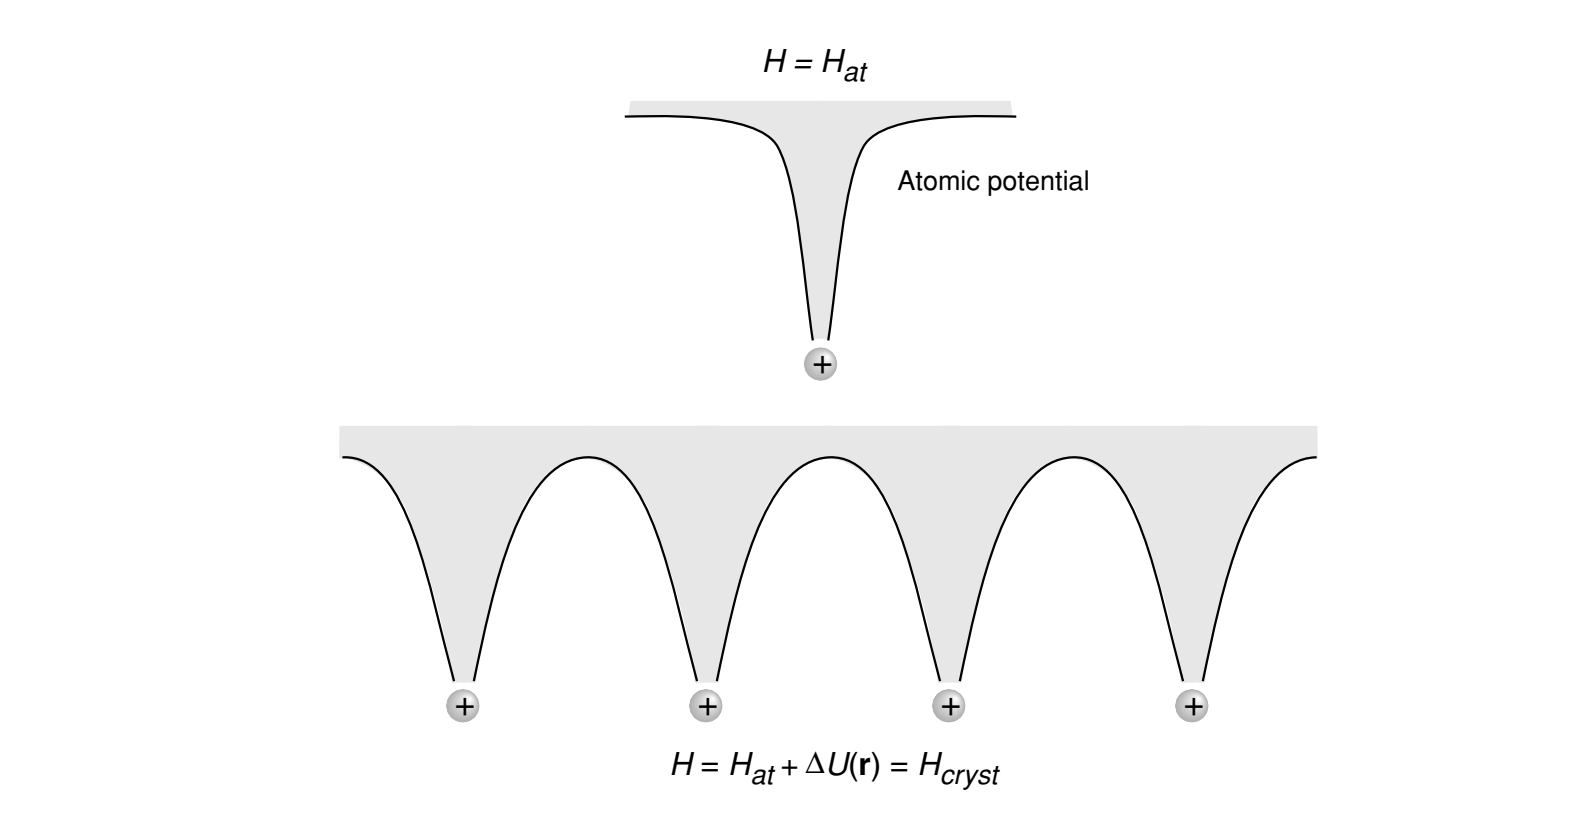
\includegraphics[width=\textwidth]{img/neighboring_atoms.png}
		\\[0.5em]
		\refstepcounter{figure}
		\textbf{Figure~\thefigure.} The effect of neighboring atoms is to perturb the atomic states, leading to the formation of bands. The perturbation is represented by \( \Delta U(\mathbf{r}) \).
		\label{fig:neighboring_atoms}
	\end{minipage}
\end{center}

The new wavefunctions must respect Bloch’s theorem and can be written in the general form:
\begin{equation}
	\Psi_{\mathbf{k}}(\mathbf{r}) = \sum_{\mathbf{R}} e^{i\mathbf{k} \cdot \mathbf{R}} \phi(\mathbf{r} - \mathbf{R})
	\label{eq:bloch_wavefunction}
\end{equation}
In this context, the function \( \phi(\mathbf{r}) \) is not itself an atomic orbital but is instead constructed as a linear combination of atomic eigenfunctions. Specifically, we can express \( \phi(\mathbf{r}) \) in terms of a finite set of atomic orbitals \( \psi_n(\mathbf{r}) \) as:
\begin{equation}
	\phi(\mathbf{r}) = \sum_{n=1}^{N} b_n \psi_n(\mathbf{r})
	\label{eq:linear_combination}
\end{equation}

\noindent
Here, \( N \) is the number of atomic orbitals included in the basis, and \( b_n \) are coefficients to be determined. In the tight binding method, only a limited number \( N \) of orbitals are retained for computational tractability.

To determine the coefficients \( b_n \), we substitute the equation above into the time-independent Schrödinger equation and derive a system of \( N \) coupled equations by projecting onto the atomic basis set. The Schrödinger equation for the crystal takes the form:
\begin{equation}
	H\Psi_{\mathbf{k}} = E(\mathbf{k}) \Psi_{\mathbf{k}}
	\label{eq:schrodinger_crystal}
\end{equation}

\noindent
Substituting Eq.\eqref{eq:bloch_wavefunction} and Eq.\eqref{eq:linear_combination}  into Eq.\eqref{eq:schrodinger_crystal}, multiplying from the left by \( \psi_m^*(\mathbf{r}) \), and integrating over all space gives:
\begin{equation}
	\int d^3 r \, \psi_m^*(\mathbf{r}) \left\{
	\left[ H_{\text{at}} + \Delta U(\mathbf{r}) \right]
	\sum_{\mathbf{R},n} b_n \, e^{i \mathbf{k} \cdot \mathbf{R}} \, \psi_n(\mathbf{r} - \mathbf{R})
	- E(\mathbf{k}) \sum_{\mathbf{R},n} b_n \, e^{i \mathbf{k} \cdot \mathbf{R}} \, \psi_n(\mathbf{r} - \mathbf{R})
	\right\} = 0
\end{equation}

\noindent
Since the atomic orbitals are orthonormal when centered on the same atom, we have:
\begin{equation}
	\int d^3r \, \psi_m^*(\mathbf{r}) \psi_n(\mathbf{r}) = \delta_{mn}
\end{equation}

\noindent
However, this orthogonality does not generally hold when the orbitals are centered at different lattice sites. That is:
\begin{equation}
	\int d^3r \, \psi_m^*(\mathbf{r}) \psi_n(\mathbf{r} - \mathbf{R}) \neq \delta_{mn} \quad \text{for} \quad \mathbf{R} \ne 0
\end{equation}

\noindent
This non-orthogonality must be accounted for in the tight binding formalism and leads to overlap integrals that influence the coupling between neighboring atomic orbitals.

In the summation over lattice vectors, we separate the terms with $\mathbf{R} = 0$ and $\mathbf{R} \neq 0$ to get,
\begin{align*}
	 & (E(\mathbf{k}) - E_m) b_m =                                                                                                                                                                           \\
	 & -(E(\mathbf{k}) - E_m) \sum_{n=1}^{N} \left( \sum_{\mathbf{R} \neq 0} \int \psi_m^*(\mathbf{r}) \, \psi_n(\mathbf{r} - \mathbf{R}) \, e^{i \mathbf{k} \cdot \mathbf{R}} \, d^3 r \right) b_n \notag   \\
	 & \quad + \sum_{n=1}^{N} \left( \int \psi_m^*(\mathbf{r}) \, \Delta U(\mathbf{r}) \, \psi_n(\mathbf{r}) \, d^3 r \right) b_n \notag                                                                     \\
	 & \quad + \sum_{n=1}^{N} \left( \sum_{\mathbf{R} \neq 0} \int \psi_m^*(\mathbf{r}) \, \Delta U(\mathbf{r}) \, \psi_n(\mathbf{r} - \mathbf{R}) \, e^{i \mathbf{k} \cdot \mathbf{R}} \, d^3 r \right) b_n
\end{align*}

It is important to recognize the use of the identity:
\begin{equation}
	\int d^3r \, \psi_m^*(\mathbf{r}) H_{\text{at}} \psi_n(\mathbf{r}) = E_m \delta_{mn}
\end{equation}

\noindent
where \( E_m \) is the energy eigenvalue associated with the atomic orbital \( \psi_m \). Note that these energies \( E_m \) may not exactly correspond to the isolated atomic energy levels, since the presence of neighboring atoms in the crystal modifies them. As such, in the tight binding method, these energies are often treated as fitting parameters to match experimental data or more accurate calculations.

An additional approximation typically made in the tight binding framework is:
\begin{equation}
	\int d^3r \, \psi_m^*(\mathbf{r}) \psi_n(\mathbf{r} - \mathbf{R}) e^{i\mathbf{k} \cdot \mathbf{R}} \approx 0
\end{equation}

\noindent
This implies that the spatial overlap between atomic orbitals centered on different atoms is negligible, which is valid when the atomic orbitals are strongly localized.

Another important concept is the \textit{on-site matrix element}, defined as:
\begin{equation}
	\int d^3r \, \psi_m^*(\mathbf{r}) H \psi_n(\mathbf{r}) = E_m + \int d^3r \, \psi_m^*(\mathbf{r}) \Delta U(\mathbf{r}) \psi_m(\mathbf{r})
\end{equation}

\noindent
For many forms of the potential \( \Delta U(\mathbf{r}) \), the integral:
\begin{equation}
	\int d^3r \, \psi_m^*(\mathbf{r}) \Delta U(\mathbf{r}) \psi_n(\mathbf{r})
\end{equation}

\noindent
vanishes when \( m \neq n \), which further simplifies the matrix elements.

To obtain the eigenvalues \( E(\mathbf{k}) \) and corresponding eigenfunctions (with coefficients \( b_n \)), we solve a system of \( N \) coupled linear equations. These form an \( N \times N \) \textit{secular equation}, from which the energy dispersion \( E(\mathbf{k}) \), or the bandstructure, can be determined. For each wavevector \( \mathbf{k} \), the solution yields \( N \) energy levels, corresponding to the bands derived from the \( N \) atomic orbitals used in the basis.

To gain intuition about this method, we next examine a simple case involving only $s$-orbitals—a so-called \textit{s-band model}.

\subsection{Tight Binding Model for s-Bands}
In the case of semiconductors, each unit cell typically contains two atoms in the basis. For each atom, it is necessary to include at least the outer shell orbitals: one \(s\)-orbital and three \(p\)-orbitals (\(p_x\), \(p_y\), and \(p_z\)). As a result, the tight binding secular equation becomes significantly more complex due to the increased number of basis functions.

To gain some intuitive understanding, we now consider a simplified model: a crystal with a single atom per unit cell and only one orbital per atom—the \(s\)-orbital. In this scenario, there is only one atomic level, and all tight binding coefficients \( \{b_n\} \) are zero except for the \(s\)-level, where \( b_s = 1 \). This simplification reduces the problem to a single equation.

We obtain:
\begin{align*}
	E(k) - E_s = & - (E(k) - E_s) \sum_{\mathbf{R} \neq 0} \int d^3r \, \psi_s^*(\mathbf{r}) \psi_s(\mathbf{r} - \mathbf{R}) e^{i\mathbf{k} \cdot \mathbf{R}}         \\
	             & + \int d^3r \, \psi_s^*(\mathbf{r}) \Delta U(\mathbf{r}) \psi_s(\mathbf{r})                                                                        \\
	             & + \sum_{\mathbf{R} \neq 0} \int d^3r \, \psi_s^*(\mathbf{r}) \Delta U(\mathbf{r}) \psi_s(\mathbf{r} - \mathbf{R}) e^{i\mathbf{k} \cdot \mathbf{R}}
\end{align*}
We define the following integrals to simplify notation:
\begin{align}
	\boxed{
		\alpha(\mathbf{R}) = \int d^3r \, \psi_s^*(\mathbf{r}) \psi_s(\mathbf{r} - \mathbf{R})
	} \\[8pt]
	\boxed{
		\beta_s = -\int d^3r \, \psi_s^*(\mathbf{r}) \Delta U(\mathbf{r}) \psi_s(\mathbf{r})
	} \\[8pt]
	\overset{\text{HOPPING INTEGRAL} \,}{\boxed{
			\gamma(\mathbf{R}) = -\int d^3r \, \psi_s^*(\mathbf{r}) \Delta U(\mathbf{r}) \psi_s(\mathbf{r} - \mathbf{R})
		}}
\end{align}

As discussed earlier, we typically neglect the overlap integral \( \alpha(\mathbf{R}) \), i.e., we set \( \alpha(\mathbf{R}) = 0 \), assuming strong localization of atomic orbitals. The energy dispersion relation simplifies to:
\begin{equation}
	\boxed{
		E(\mathbf{k}) = E_s - \beta - \sum_{\mathbf{R}} \gamma(\mathbf{R}) e^{i\mathbf{k} \cdot \mathbf{R}}}
\end{equation}
The off-site matrix elements \( \gamma(\mathbf{R}) \) decay rapidly with increasing distance \( \mathbf{R} \), so we consider only the nearest-neighbor interactions. Additionally, due to lattice symmetry, \( \gamma(-\mathbf{R}) = \gamma(\mathbf{R}) \).

Let us now apply this to a face-centered cubic (fcc) lattice. The twelve nearest neighbors of a lattice site in an fcc crystal are located at:
\begin{equation*}
	\frac{a}{2} (\pm1, \pm1, 0), \quad \frac{a}{2} (\pm1, 0, \pm1), \quad \frac{a}{2} (0, \pm1, \pm1)
\end{equation*}
Taking into account all twelve neighbors, the energy becomes:
\begin{align*}
	E(\mathbf{k}) & = E_s - \beta - \gamma \sum_{\mathbf{R}} e^{i\mathbf{k} \cdot \mathbf{R}}                                                                                                                                                                                \\
	              & = E_s - \beta - \boxed{4\gamma} \left[ \cos\left(\frac{k_x a}{2}\right) \cos\left(\frac{k_y a}{2}\right) + \cos\left(\frac{k_y a}{2}\right) \cos\left(\frac{k_z a}{2}\right) + \cos\left(\frac{k_z a}{2}\right) \cos\left(\frac{k_x a}{2}\right) \right]
\end{align*}
This final expression captures \textbf{the energy dispersion relation} for an \(s\)-band in an fcc lattice, considering only nearest-neighbor interactions.

We now analyze the energy band derived above within the context of the first Brillouin zone of the face-centered cubic (fcc) lattice.
From the geometry of the Brillouin zone, we observe that there are six equivalent \( X \)-points and eight equivalent \( L \)-points, which are critical in determining the behavior of the electronic bandstructure.\\
By evaluating the energy expression from the last relation obtained along various high-symmetry directions in \( \mathbf{k} \)-space, we can obtain the band dispersion throughout the Brillouin zone. The resulting energy bands reflect the symmetry of the lattice and provide insight into the electronic properties of the material.
\begin{center}
	\begin{minipage}{0.9\textwidth}
		\centering
		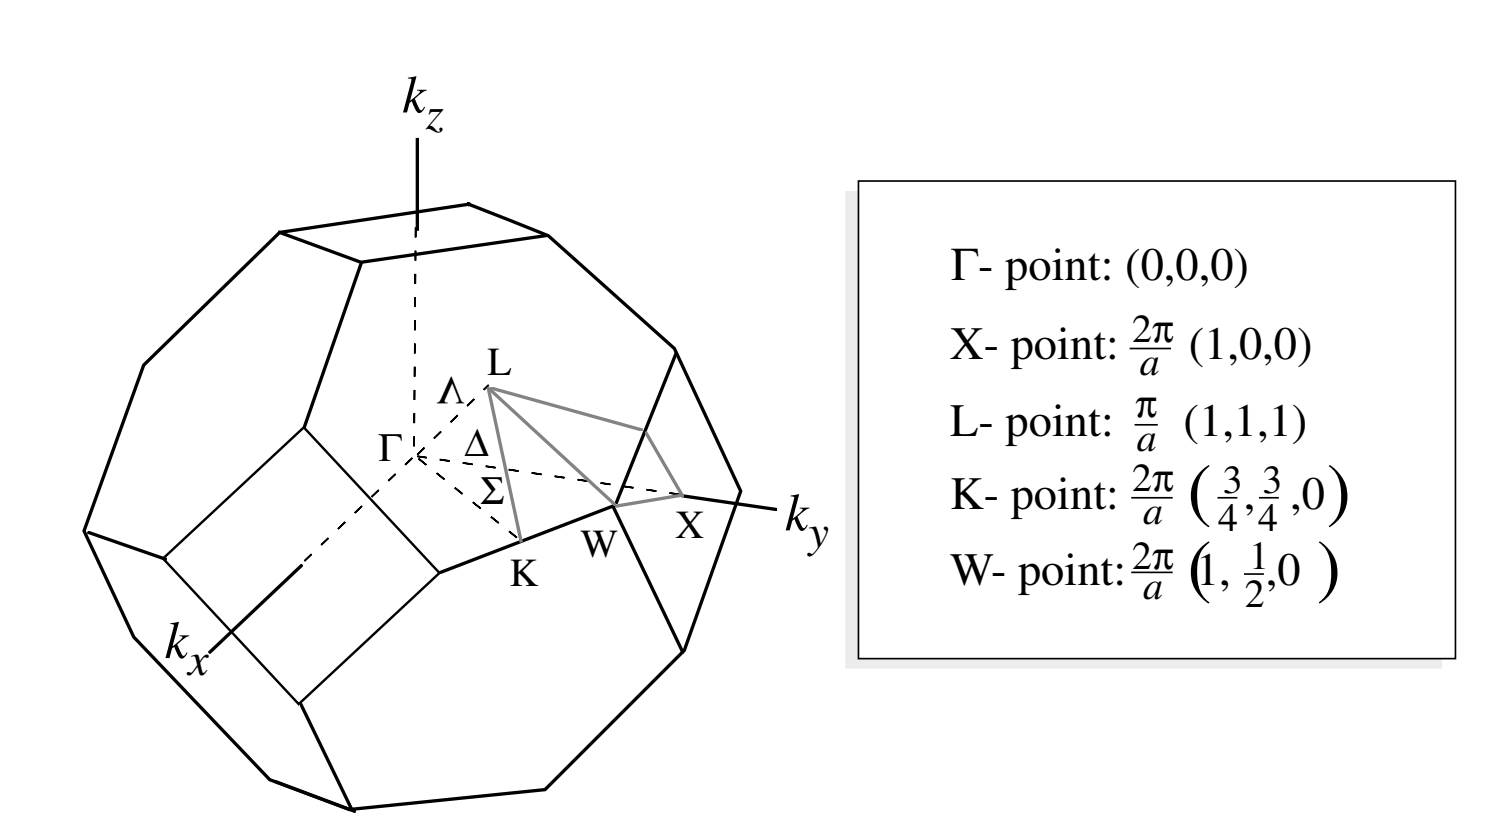
\includegraphics[width=\textwidth]{img/BrillouinZones.png}
		\\[0.5em]
		\refstepcounter{figure}
		\textbf{Figure~\thefigure.} Brillouin zones of the face-centered cubic (fcc) lattice. The high-symmetry points \( \Gamma \), \( X \), and \( L \) are indicated, along with their corresponding coordinates in reciprocal space.
		\label{fig:BrillouinZones}
	\end{minipage}
\end{center}

To further understand the nature of the bandstructure, we examine the dispersion relation \( E(\mathbf{k}) \) along key high-symmetry directions in the first Brillouin zone of the fcc lattice. These paths correspond to the directions \( \Gamma \rightarrow X \), \( \Gamma \rightarrow L \), and \( \Gamma \rightarrow K \), and the corresponding energy expressions can be obtained by substituting specific components of \( \mathbf{k} \) into Eq.~(2.35).

\begin{itemize}
	\item \textbf{Along \( \Gamma X \)}: Set \( k_x = \frac{2\pi \alpha}{a} \), \( k_y = k_z = 0 \), with \( 0 \leq \alpha \leq 1 \). The energy becomes:
	      \begin{equation*}
		      E(\mathbf{k}) = E_s - \beta - 4\gamma (1 + 2 \cos \pi \alpha)
	      \end{equation*}
	\item \textbf{Along \( \Gamma L \)}: Set \( k_x = k_y = k_z = \frac{2\pi \alpha}{a} \), with \( 0 \leq \alpha \leq \frac{1}{2} \). The energy expression is:
	      \begin{equation*}
		      E(\mathbf{k}) = E_s - \beta - 12\gamma \cos^2(\pi \alpha)
	      \end{equation*}
	\item \textbf{Along \( \Gamma K \)}: Set \( k_x = k_y = \frac{2\pi \alpha}{a} \), \( k_z = 0 \), with \( 0 \leq \alpha \leq \frac{3}{4} \). The energy becomes:
	      \begin{equation*}
		      E(\mathbf{k}) = E_s - \beta - 4\gamma \left( \cos^2 \pi \alpha + 2 \cos\left( \frac{\pi \alpha}{2} \right) \right)
	      \end{equation*}
\end{itemize}

The bandstructure—i.e., the relation between energy \( E \) and wavevector \( \mathbf{k} \)—is typically plotted along these high-symmetry paths, as shown in Fig.\ref{fig:BrillouinZones}. In the illustrative case where \( \gamma = 1.0\,\text{eV} \) and \( E_s + \beta = 0 \), the resulting bandwidth is found to be:
\begin{equation*}
	\Delta E = 16\gamma
\end{equation*}
This shows that greater overlap between neighboring atomic orbitals (i.e., larger \( \gamma \)) leads to wider energy bands.
It is particularly useful to analyze the bandstructure near the \( \Gamma \) point, where the wavevector \( \mathbf{k} \) is small. By choosing \( k_x = k_y = k_z = k/\sqrt{3} \) such that \( ka \ll 1 \), the cosine terms can be expanded, yielding:
\begin{equation}
	E(\mathbf{k}) = E_s - \beta - 12\gamma + \gamma a^2 k^2
\end{equation}
Comparing this expression with the free electron dispersion relation:
\begin{equation*}
	E(p) = E_0 + \frac{p^2}{2m}
\end{equation*}
\noindent
we can rewrite the tight binding result in a similar form:
\begin{equation*}
	E(\mathbf{k}) = E_s - \beta - 12\gamma + \frac{\hbar^2 k^2}{2 m^*}
\end{equation*}
This allows us to define an effective mass \( m^* \) for the electrons near the bottom of the band:
\begin{equation}
	m^* = \frac{\hbar^2}{2\gamma a^2}
\end{equation}
\noindent
This effective mass characterizes the curvature of the band near \( \Gamma \) and plays a central role in transport phenomena in semiconductors.
\begin{center}
	\begin{minipage}{0.6\textwidth}
		\centering
		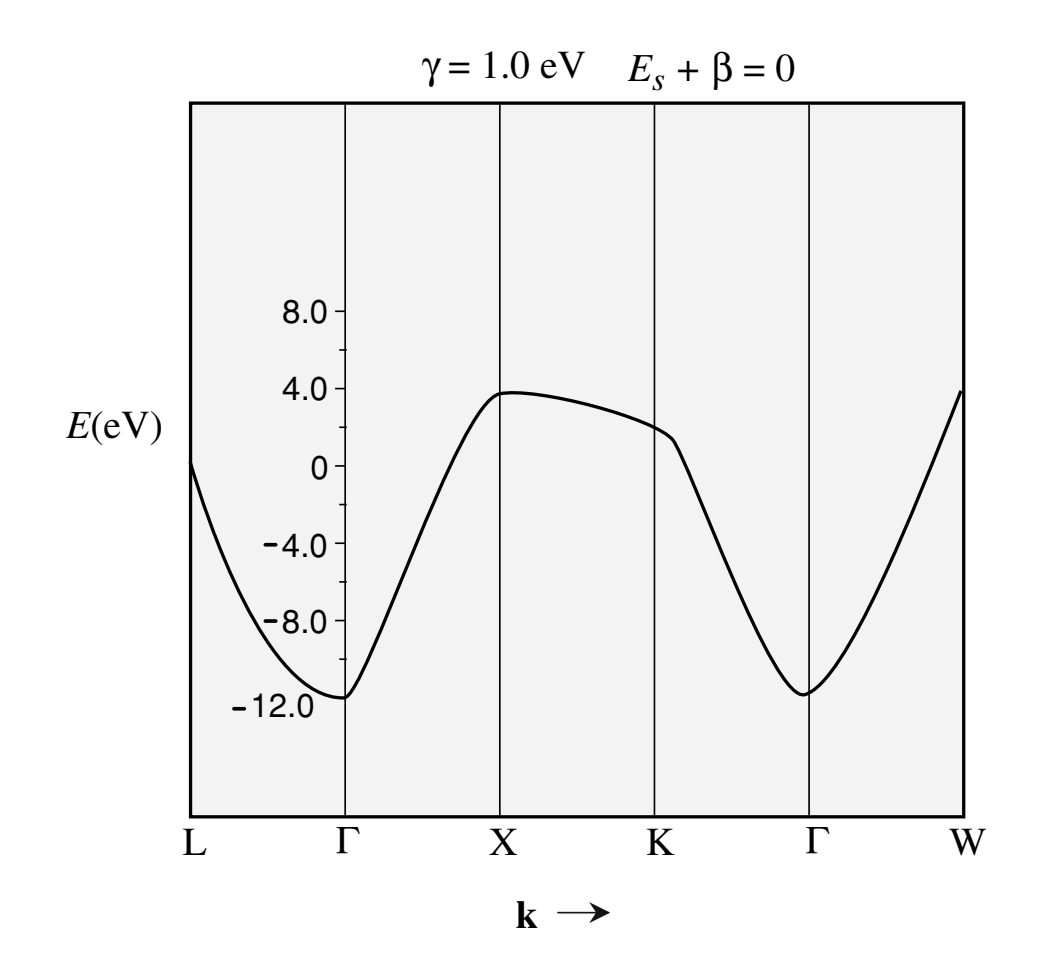
\includegraphics[width=\textwidth]{img/s-band-model.png}
		\\[0.5em]
		\refstepcounter{figure}
		\textbf{Figure~\thefigure.} Bandstructure of an \(s\)-band in a face-centered cubic (fcc) lattice. The energy dispersion is plotted along high-symmetry directions in the Brillouin zone, illustrating the relationship between energy \( E \) and wavevector \( \mathbf{k} \). The effective mass \( m^* \) is defined near the \( \Gamma \) point.
		\label{fig:s-band-model}
	\end{minipage}
\end{center}


\subsection{Bandstructure of Semiconductors}
We now extend the discussion of TBM to semiconductor materials. As previously mentioned, the outermost electrons in semiconductors are typically described using atomic orbitals of type \( s \), \( p_x \), \( p_y \), and \( p_z \). The accuracy of the method can be improved by including additional atomic states, though the minimal useful basis already captures much of the essential physics.

In semiconductor crystals, there are typically two atoms per unit cell. Therefore, to describe the central-cell portion of the Bloch functions, we require a total of eight atomic orbitals—four per atom. We construct the Bloch-like wavefunction as:
\begin{equation}
	\Psi(\mathbf{k}, \mathbf{r}) = \sum_{R_i} \sum_{j=1}^{2} \sum_{m=1}^{4} C_{mj}(\mathbf{k}) \, \phi_{mj}(\mathbf{r} - \mathbf{r}_j - \mathbf{R}_i) \, e^{i\mathbf{k} \cdot \mathbf{R}_i}
\end{equation}
\noindent
Here, \( \mathbf{R}_i \) runs over the lattice vectors, \( j \) indexes the atoms within each unit cell, \( m \) refers to the atomic orbital type (\( s, p_x, p_y, p_z \)), and \( \phi_{mj} \) are the atomic-like basis functions centered at position \( \mathbf{r}_j \) in the unit cell. The coefficients \( C_{mj}(\mathbf{k}) \) are to be determined by solving the Schrödinger equation.\\
As done in the simpler \( s \)-band case, we now formulate the Schrödinger equation as a matrix eigenvalue problem in the form of a secular determinant:
\begin{equation}
	\left| \langle \phi_{mj} | H - E(\mathbf{k}) | \Psi(\mathbf{k}) \rangle \right| = 0
\end{equation}
\noindent
Here, \( H \) is the crystal Hamiltonian, and the determinant must vanish for nontrivial solutions to exist.

In the tight binding method (TBM) applied to zinc–blende crystals using an \( sp^3 \) basis, the wavefunction is constructed from eight atomic orbitals: one \( s \)-orbital and three \( p \)-orbitals (\( p_x, p_y, p_z \)) for each of the two atoms in the Wigner–Seitz cell. This results in a total of eight basis functions per unit cell.\\

This formulation assumes that the bandstructure exhibits spin degeneracy—that is, each electronic state is doubly degenerate due to the presence of both spin-up and spin-down electrons. If one wishes to include the effects of spin–orbit coupling or any interaction that breaks spin degeneracy, the basis must be expanded accordingly.\\

In the tight binding approximation, the top of the valence band is predicted to be three-fold degenerate, corresponding to the degeneracy of the \( p_x \), \( p_y \), and \( p_z \) orbitals. When spin is taken into account, this degeneracy becomes six-fold, since each orbital state can have both spin-up and spin-down components.\\

However, experimental observations and more accurate theoretical models show that, in most semiconductors, the top of the valence band is actually two-fold degenerate (four-fold with spin). Additionally, there exists another band—also two-fold degenerate—that lies slightly below the valence band maximum.
These features cannot be captured by a purely non-relativistic tight binding model. To accurately reproduce this band splitting, relativistic effects must be incorporated. The interaction responsible for this splitting is known as \textit{spin–orbit coupling}, which lifts part of the degeneracy by coupling the electron's spin and orbital angular momentum.

\begin{center}
	\begin{minipage}{0.6\textwidth}
		\centering
		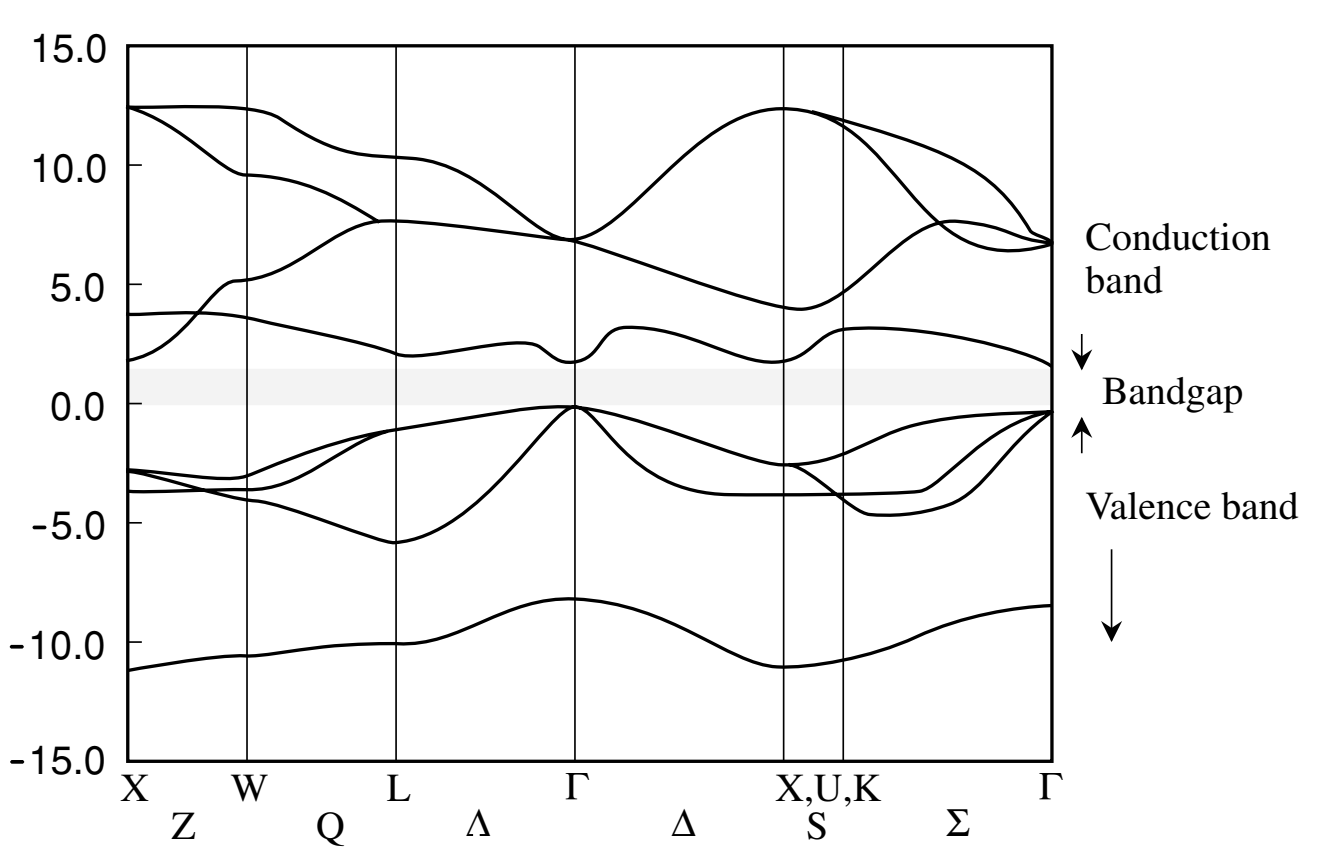
\includegraphics[width=\textwidth]{img/GaAs_TBM.png}
		\\[0.5em]
		\refstepcounter{figure}
		\textbf{Figure~\thefigure.} Band structure of GaAs obtained using the tight-binding model, excluding spin-orbit interaction. As shown, this approach alone does not provide a precise description of the valence band edge unless spin-orbit effects are taken into account.
		\label{fig:GaAs_TBM}
	\end{minipage}
\end{center}

\section{Spin-Orbit Coupling}
In nearly all semiconductors, it is observed that the states at the top of the valence band are predominantly derived from \( p \)-type atomic orbitals. Consequently, any bandstructure calculation that does not include spin effects tends to produce an inaccurate description of the valence band. The spin degree of freedom allows the electron to interact with the magnetic field generated by its own orbital motion.

An electron occupying a \( p \)-orbital possesses a non-zero orbital angular momentum \( \hbar \), which leads to a significant coupling between its spin and orbital motion. Since the valence band maximum is mainly composed of such \( p \)-like states, spin–orbit coupling has a pronounced influence in this energy region.

While the spin–orbit interaction can be calculated fairly accurately for isolated atoms, performing such calculations for crystalline solids is more complex. Therefore, in practical applications, the spin–orbit interaction is often incorporated through an effective model that uses a fitting parameter \( \lambda \), adjusted to match experimental results. In many materials, the magnitude of this interaction is relatively small, and its effects can be treated perturbatively.

When including the spin–orbit interaction in the tight binding Hamiltonian, the total Hamiltonian takes the form:
\begin{equation}
	H = H_{\text{tb}} + H_{\text{so}}
\end{equation}
\noindent
where \( H_{\text{tb}} \) is the tight binding Hamiltonian, and \( H_{\text{so}} \) represents the spin–orbit coupling term. This additional term can induce coupling between states of different spin. A commonly used model for this interaction is:
\begin{equation*}
	H_{\text{so}} = \lambda \, \mathbf{L} \cdot \mathbf{S}
\end{equation*}
\noindent
Here, \( \mathbf{L} \) is the orbital angular momentum operator, \( \mathbf{S} \) is the spin angular momentum operator, and \( \lambda \) is a material-dependent constant representing the strength of the interaction.\\
The total angular momentum operator \( \mathbf{J} \) is defined as:
\begin{equation}
	\mathbf{J} = (\mathbf{L} + \mathbf{S})^2 = \mathbf{L}^2 + \mathbf{S}^2 + 2 \mathbf{L} \cdot \mathbf{S}
\end{equation}
\noindent
Using this, we can derive the expectation value of \( \mathbf{L} \cdot \mathbf{S} \) as:
\begin{equation*}
	\langle \mathbf{L} \cdot \mathbf{S} \rangle = \frac{1}{2} \left[ J^2 - L^2 - S^2 \right]
\end{equation*}
\noindent
which leads to:
\begin{equation}
	\langle \mathbf{L} \cdot \mathbf{S} \rangle = \frac{\hbar^2}{2} \left[ j(j + 1) - l(l + 1) - s(s + 1) \right]
\end{equation}

\noindent
Here, \( j \), \( l \), and \( s \) are the quantum numbers corresponding to the total, orbital, and spin angular momentum, respectively. This relation provides a straightforward way to estimate the spin–orbit interaction energy—provided the states are characterized by well-defined angular momentum quantum numbers.\\
However, it is important to note that many states in solids, such as a \( p^\uparrow \) state, are not pure eigenstates of \( \mathbf{J} \), but rather are mixed combinations of such states. In these cases, a more detailed analysis is required to fully account for the spin–orbit coupling effects.

The spin–orbit Hamiltonian can be expressed in terms of the quantum numbers associated with total, orbital, and spin angular momentum as:
\begin{equation}
	H_{\text{so}} = \frac{\lambda \hbar^2}{2} \left[ j(j + 1) - l(l + 1) - s(s + 1) \right]
\end{equation}

\noindent
For electrons in \( p \)-type orbitals, we have \( l = 1 \) and \( s = \frac{1}{2} \). The value of \( j \) depends on the specific total angular momentum eigenstate, and is determined by the decomposition of the mixed states into pure angular momentum components.\\
Due to the orthogonality of the total angular momentum eigenstates, many cross terms in matrix element calculations vanish, simplifying the application of the spin–orbit interaction to the bandstructure problem.

The influence of spin–orbit coupling is more clearly illustrated when the states are described in the total angular momentum basis, rather than in the \( p_x \), \( p_y \), and \( p_z \) orbital basis. In this representation, the \( p \)-orbitals (including spin) correspond to six states of the form \( |j, m\rangle \), where \( j \) is the total angular momentum quantum number and \( m \) is its projection.\\
These six states are:
\begin{equation*}
	|3/2, +3/2\rangle, \quad |3/2, -3/2\rangle, \quad |3/2, +1/2\rangle, \quad |3/2, -1/2\rangle, \quad |1/2, +1/2\rangle, \quad |1/2, -1/2\rangle
\end{equation*}
As follows from the spin–orbit Hamiltonian, this interaction splits the six degenerate \( p \)-states into two distinct sets: a quartet with \( j = 3/2 \), and a doublet with \( j = 1/2 \). The energy separation between these two groups is denoted by \( \Delta_{so} \), known as the spin–orbit splitting.\\
At the valence band edge of semiconductors, this results in a two-fold degenerate state (four-fold including spin) at the zone center, and a lower-energy two-fold degenerate split-off band. The upper set of degenerate states possesses different effective masses, which gives rise to the so-called \textit{light hole} (LH) and \textit{heavy hole} (HH) bands.\\
This spin–orbit-induced splitting is a key feature in the accurate description of valence band structure in semiconductors.

\begin{figure}[h!]
	\centering
	\begin{minipage}{0.48\textwidth}
		\centering
		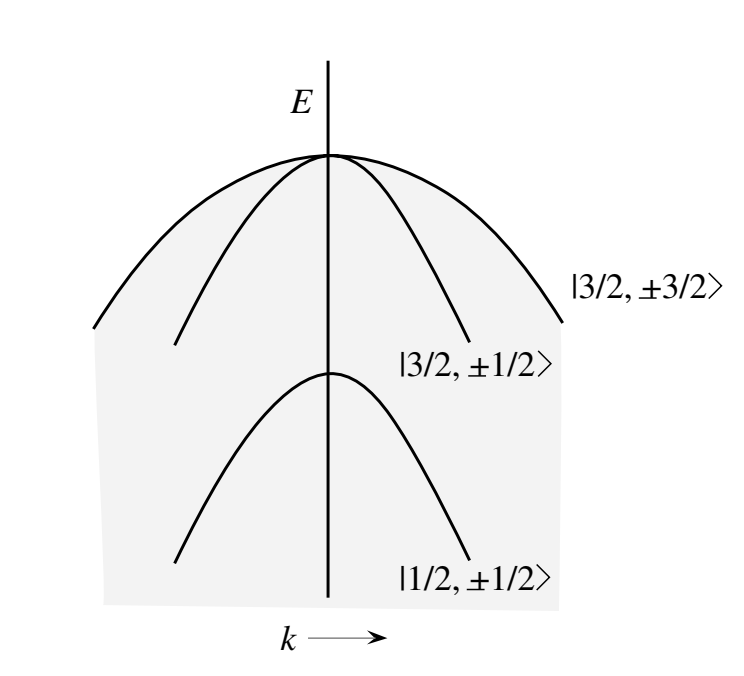
\includegraphics[width=\textwidth]{img/valence_bandstructure.png}
		\\[0.5em]
		\refstepcounter{figure}
		\textbf{Figure~\thefigure.} The general form of the valence bandstructure after incorporating spin--orbit coupling. At the Brillouin zone center ($\mathbf{k} = 0$), the electronic states exhibit well-defined angular momentum character.
		\label{fig:valence_bandstructure}
	\end{minipage}%
	\hfill
	\begin{minipage}{0.48\textwidth}
		\centering
		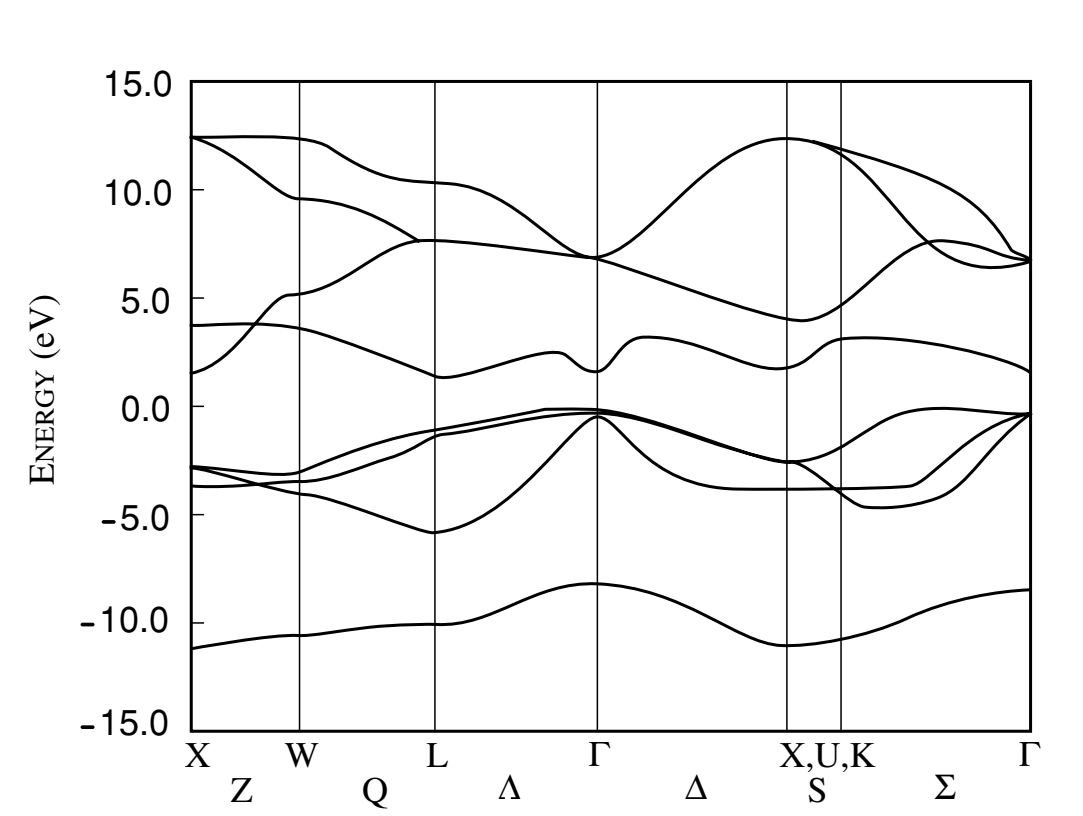
\includegraphics[width=\textwidth]{img/GaAs-spinorbit.png}
		\\[0.5em]
		\refstepcounter{figure}
		\textbf{Figure~\thefigure.} Tight-binding bandstructure of GaAs computed with spin--orbit coupling included. The degeneracy between the light-hole, heavy-hole, and split-off bands is lifted as a result of the spin--orbit interaction.
		\label{fig:GaAs_spin_orbit}
	\end{minipage}
\end{figure}


\subsection{Symmetry of Bandedge States}
In direct bandgap semiconductors, the conduction band minimum occurs at the \( \Gamma \)-point. The periodic part of the Bloch wavefunction at this point is spherically symmetric and primarily composed of \( s \)-type atomic orbitals. As one moves away from the band edge, the eigenstates acquire increasing contributions from \( p \)-type orbitals. However, the dominant \( s \)-character near the conduction band edge gives rise to important optical transition selection rules, which will be discussed in more detail later.

In contrast, indirect bandgap semiconductors such as silicon and germanium exhibit conduction band minima away from the \( \Gamma \)-point. In silicon, the minimum lies near the \( X \)-point and is six-fold degenerate, while in germanium it occurs at the \( L \)-point. The electronic states at these minima are highly anisotropic and involve complex combinations of \( s \)- and \( p \)-type orbitals (\( p_x \), \( p_y \), and \( p_z \)) in their wavefunction composition.

Despite the differences in conduction band behavior, the valence band edge structure in most semiconductors is qualitatively similar. The periodic component of the wavefunction at the valence band maximum is primarily \( p \)-type, which enhances the influence of spin–orbit coupling in this region.

In the absence of spin–orbit interaction, the top of the valence band is three-fold degenerate (six-fold when spin degeneracy is included). When spin–orbit coupling is taken into account, this degeneracy is lifted, resulting in a four-fold degenerate manifold at the top of the valence band and a lower two-fold degenerate split-off band. The upper four-fold degenerate states comprise the heavy hole (HH) and light hole (LH) bands, while the lower-lying two-fold degenerate states form the split-off band.
\subsection*{Heavy hole states}
\begin{equation}
	\boxed{
		\Phi_{3/2, +3/2} = -\frac{1}{\sqrt{2}} \left( |p_x\rangle + i |p_y\rangle \right) |\uparrow\rangle
	}
\end{equation}

\begin{equation}
	\boxed{
		\Phi_{3/2, -3/2} = \frac{1}{\sqrt{2}} \left( |p_x\rangle - i |p_y\rangle \right) |\downarrow\rangle
	}
\end{equation}

\subsection*{Light hole states}
\begin{equation}
	\boxed{
		\Phi_{3/2, +1/2} = -\frac{1}{\sqrt{6}} \left[ \left( |p_x\rangle + i |p_y\rangle \right) |\downarrow\rangle - 2 |p_z\rangle |\uparrow\rangle \right]
	}
\end{equation}

\begin{equation}
	\boxed{
		\Phi_{3/2, -1/2} = \frac{1}{\sqrt{6}} \left[ \left( |p_x\rangle - i |p_y\rangle \right) |\uparrow\rangle + 2 |p_z\rangle |\downarrow\rangle \right]
	}
\end{equation}

\subsection*{Split-off hole states}
\begin{equation}
	\boxed{
		\Phi_{1/2, +1/2} = -\frac{1}{\sqrt{3}} \left[ \left( |p_x\rangle + i |p_y\rangle \right) |\downarrow\rangle + |p_z\rangle |\uparrow\rangle \right]
	}
\end{equation}

\begin{equation}
	\boxed{
		\Phi_{1/2, -1/2} = \frac{1}{\sqrt{3}} \left[ \left( |p_x\rangle - i |p_y\rangle \right) |\uparrow\rangle + |p_z\rangle |\downarrow\rangle \right]
	}
\end{equation}

\begin{center}
	\begin{minipage}{0.9\textwidth}
		\centering
		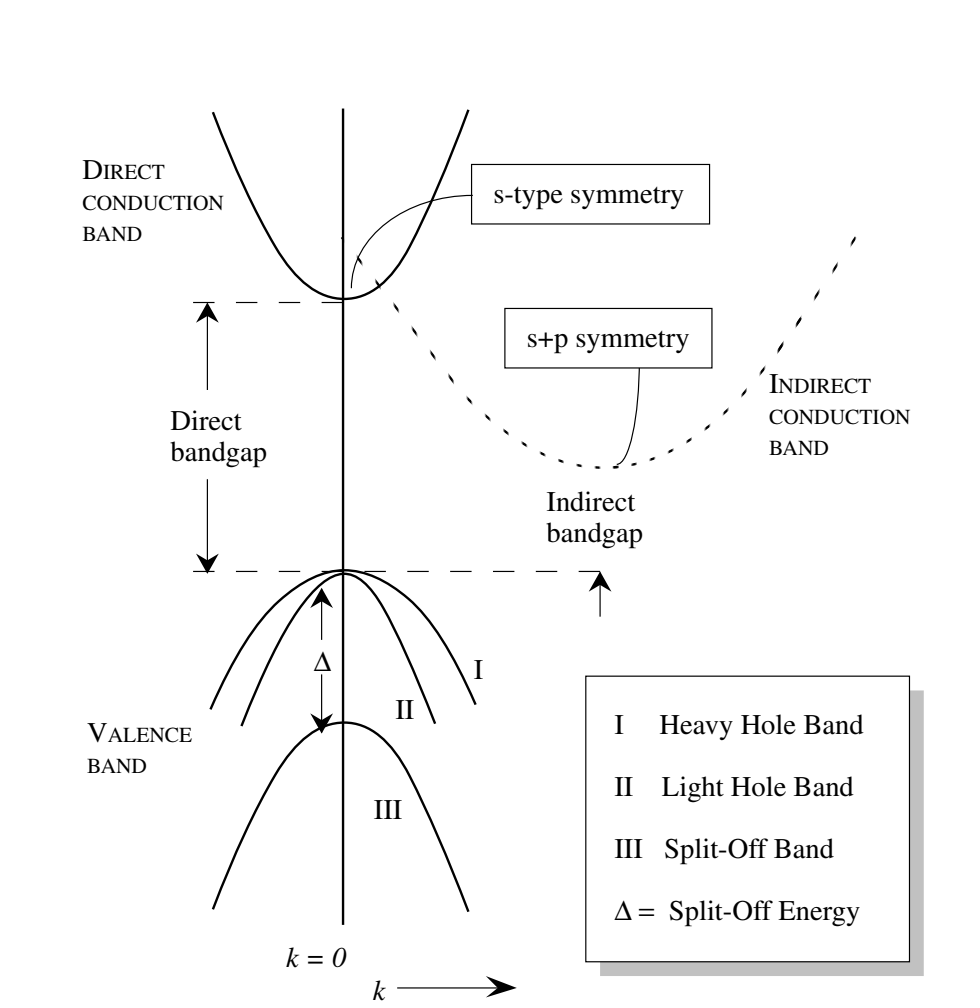
\includegraphics[width=\textwidth]{img/general_valenceband.png}
		\\[0.5em]
		\refstepcounter{figure}
		\textbf{Figure~\thefigure.} Schematic of the valence band and conduction bands in direct and indirect bandgap semiconductors. Solid and dashed lines represent the conduction bands of direct and indirect materials, respectively.
		\label{fig:general_valenceband}
	\end{minipage}
\end{center}

\section{Selected Bandstructures}
\subsection{Silicon}
Silicon forms the foundational material of the modern electronics industry. A key feature of silicon is that it possesses an indirect bandgap, which significantly limits its usefulness in optical applications—particularly for light-emitting devices.\\
The conduction band minimum in silicon does not occur at the \( \Gamma \)-point, but rather near the \( X \)-point in the Brillouin zone, approximately at \( (2\pi/a)(0.85, 0, 0) \). There are six equivalent \( X \)-points in the Brillouin zone, leading to six degenerate conduction band valleys. As a result, the conduction band edge in silicon exhibits a multi-valley structure.\\
Near the conduction band edge, the periodic part of the Bloch wavefunctions exhibits a strong mixture of \( s \)- and \( p \)-type character. Specifically, along the longitudinal direction (aligned with the valley axis, e.g., the \( x \)-axis for the [100] valley), the states have contributions from \( s \)- and \( p_x \)-type orbitals. In the transverse directions (\( y \) and \( z \)), the wavefunction is composed primarily of \( p_y \)- and \( p_z \)-like components.\\
Close to the band edge, the energy dispersion relation can be approximated by an ellipsoidal form. For a given valley aligned along the [100] direction, the energy as a function of wavevector \( \mathbf{k} \) is given by:
\begin{equation}
	E(\mathbf{k}) = \frac{\hbar^2 k_x^2}{2 m_l^*} + \frac{\hbar^2}{2 m_t^*} \left( k_y^2 + k_z^2 \right)
\end{equation}
\noindent
Here, \( m_l^* \) is the effective mass along the longitudinal axis of the ellipsoid (parallel to the valley direction), and \( m_t^* \) is the effective mass in the transverse directions. This anisotropic mass behavior reflects the ellipsoidal constant-energy surfaces around each conduction band minimum.
\begin{center}
	\begin{minipage}{0.7\textwidth}
		\centering
		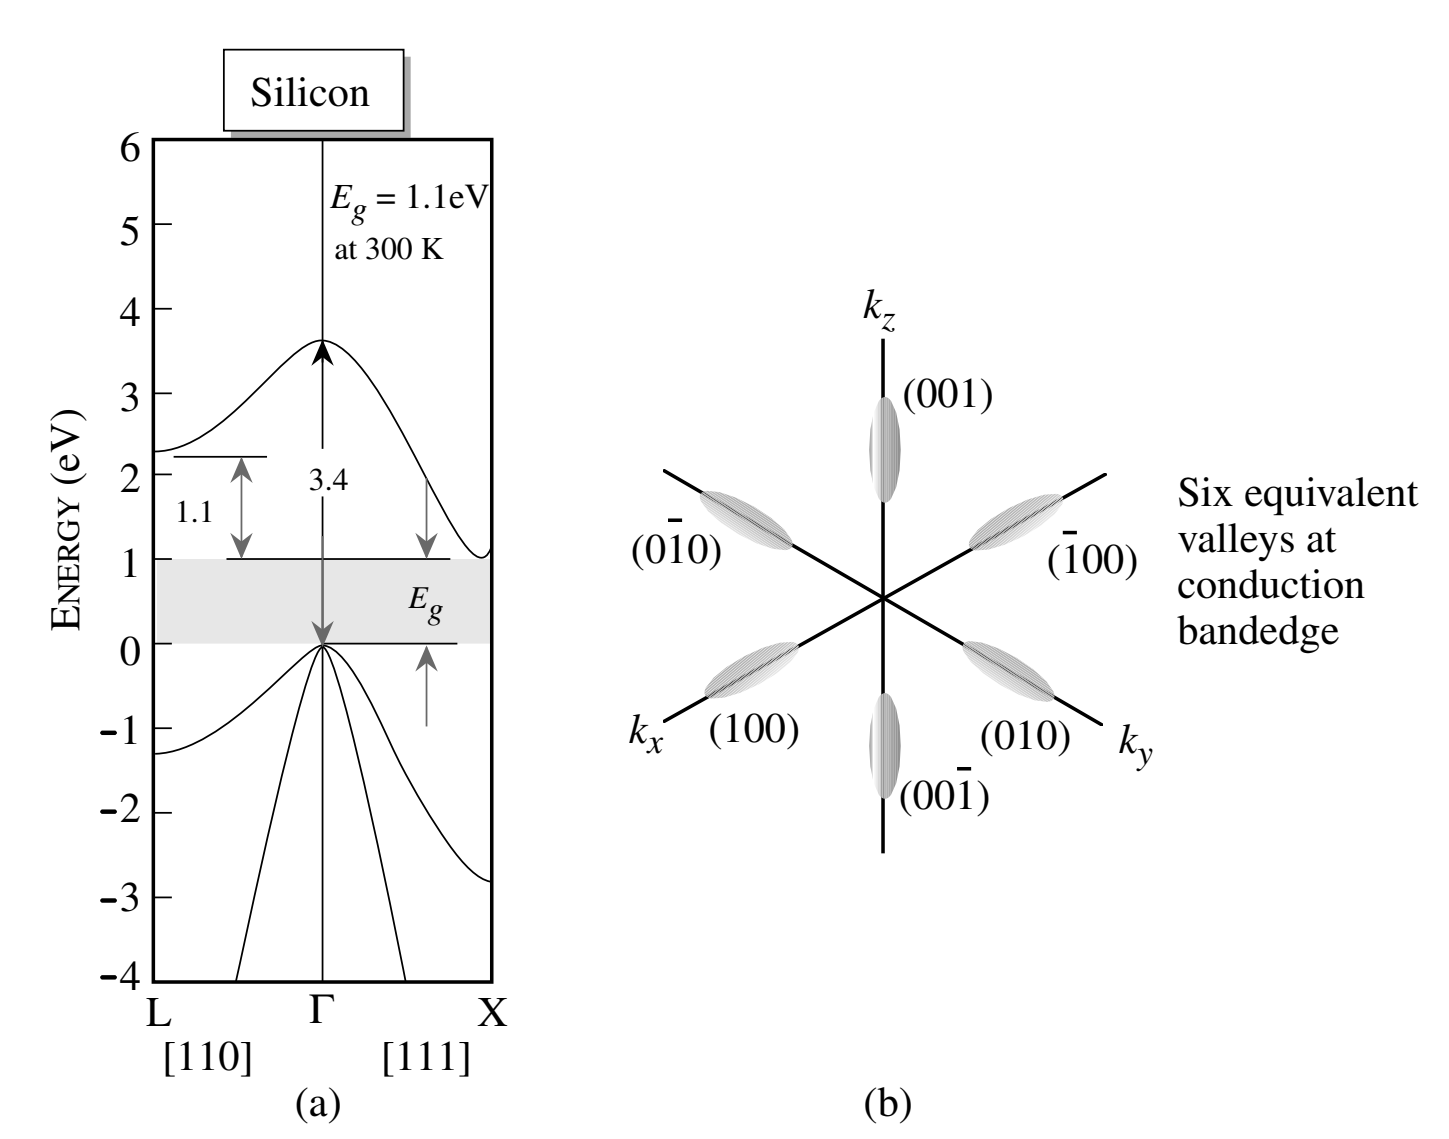
\includegraphics[width=\textwidth]{img/silicon.png}
		\\[0.5em]
		\refstepcounter{figure}
		\textbf{Figure~\thefigure.}
		\label{fig:Silicon}
	\end{minipage}
\end{center}

\subsection{GaAs}
The bandstructure near the band edge in GaAs is characterized by a direct bandgap located at the \( \Gamma \)-point. This direct bandgap is one of the key reasons for the technological relevance of GaAs, as it enables excellent optical properties and high electron mobility in the conduction band.\\
Near the conduction band minimum at \( \Gamma \), the energy-momentum relationship can be approximated by the simple parabolic form:
\begin{equation*}
	E = \frac{\hbar^2 k^2}{2 m^*}
\end{equation*}
\noindent
with an effective mass \( m^* = 0.067 m_0 \), where \( m_0 \) is the free electron mass.\\
A more accurate representation, especially at higher energies, is provided by the nonparabolic dispersion relation:
\begin{equation*}
	E(1 + \alpha E) = \frac{\hbar^2 k^2}{2 m^*}
\end{equation*}
\noindent
where the nonparabolicity parameter \( \alpha \) has a value of approximately \( 0.67\, \text{eV}^{-1} \).\\
For high electric field transport, it is important to consider higher energy conduction band valleys. Above the \( \Gamma \)-valley lie the \( L \)-valleys. There are eight equivalent \( L \)-points in the Brillouin zone, but due to equivalence under reciprocal lattice translations, only four of these are distinct. The energy separation between the \( \Gamma \) minimum and the \( L \)-valleys is approximately \( \Delta E_{\Gamma L} = 0.29\, \text{eV} \). The effective mass in the \( L \)-valley is significantly larger than at \( \Gamma \), with:
\begin{equation}
	m^*_{L} \approx 0.25\, m_0
\end{equation}
This mass difference plays a crucial role in high-field transport behavior, including the onset of negative differential resistance. At still higher energies lies the \( X \)-valley, separated from \( \Gamma \) by approximately \( \Delta E_{\Gamma X} \approx 0.58\, \text{eV} \). The effective mass in the \( X \)-valley is also large:
\begin{equation}
	m^*_{X} \approx 0.6\, m_0
\end{equation}
Under high electric fields, electrons can be transferred from the \( \Gamma \)-valley into the higher-energy \( L \) and \( X \) valleys, making these regions of the conduction band particularly important for transport properties.\\
The valence band in GaAs exhibits the standard structure consisting of heavy hole (HH), light hole (LH), and split-off (SO) bands. Due to the relatively large spin–orbit splitting in GaAs, the SO band lies significantly lower in energy and generally does not contribute to electronic or optoelectronic processes under typical operating conditions.\\
The valence band structure can be described using the Kohn–Luttinger parameters for GaAs, which are:
\begin{align*}
	\gamma_1 & = 6.85 \\
	\gamma_2 & = 2.10 \\
	\gamma_3 & = 2.90
\end{align*}
These parameters yield the following density-of-states effective masses for holes:
\begin{align*}
	m^*_{\text{HH}} & = 0.45\, m_0 \\
	m^*_{\text{LH}} & = 0.08\, m_0
\end{align*}
As with silicon, the hole effective masses in GaAs are highly anisotropic, and the \( E(\mathbf{k}) \) relation for holes reflects this anisotropy in both curvature and carrier dynamics.
\begin{figure}[h!]
	\centering
	\begin{minipage}{0.36\textwidth}
		\centering
		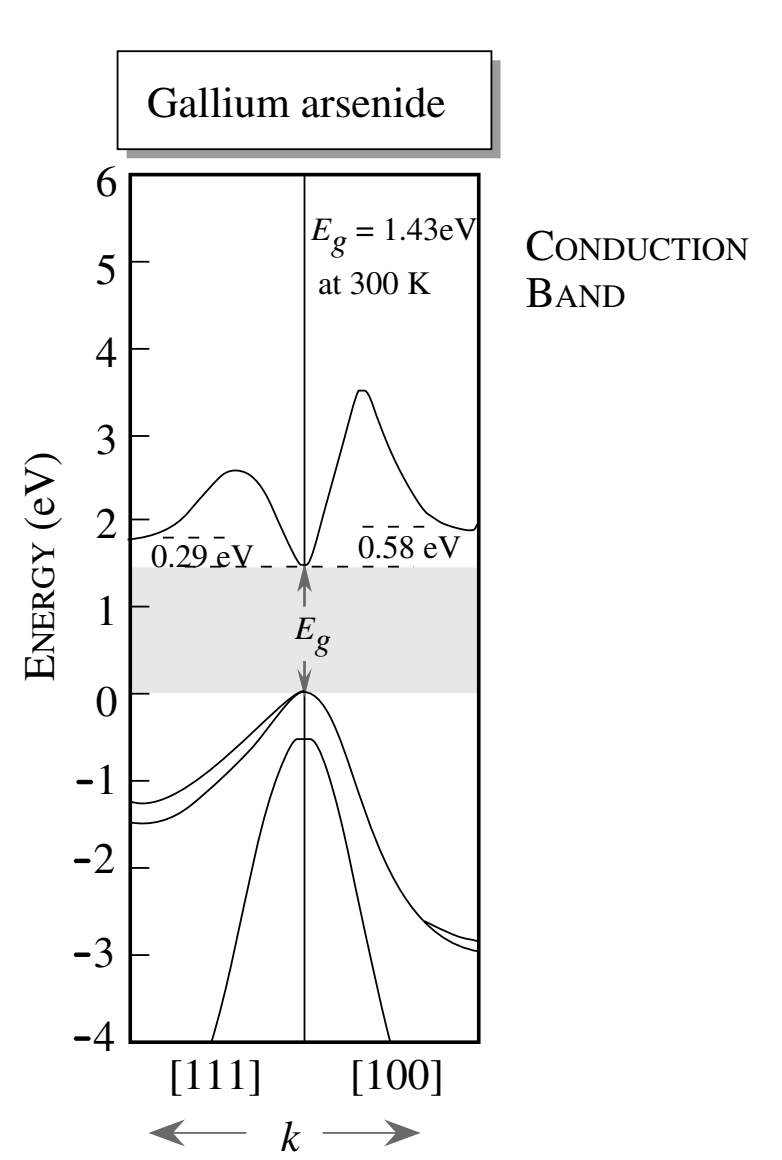
\includegraphics[width=\textwidth]{img/Gallium.png}
		\\[0.5em]
		\refstepcounter{figure}
		\textbf{Figure~\thefigure.}
		\label{fig:Gallium}
	\end{minipage}%
	\hfill
	\begin{minipage}{0.64\textwidth}
		\centering
		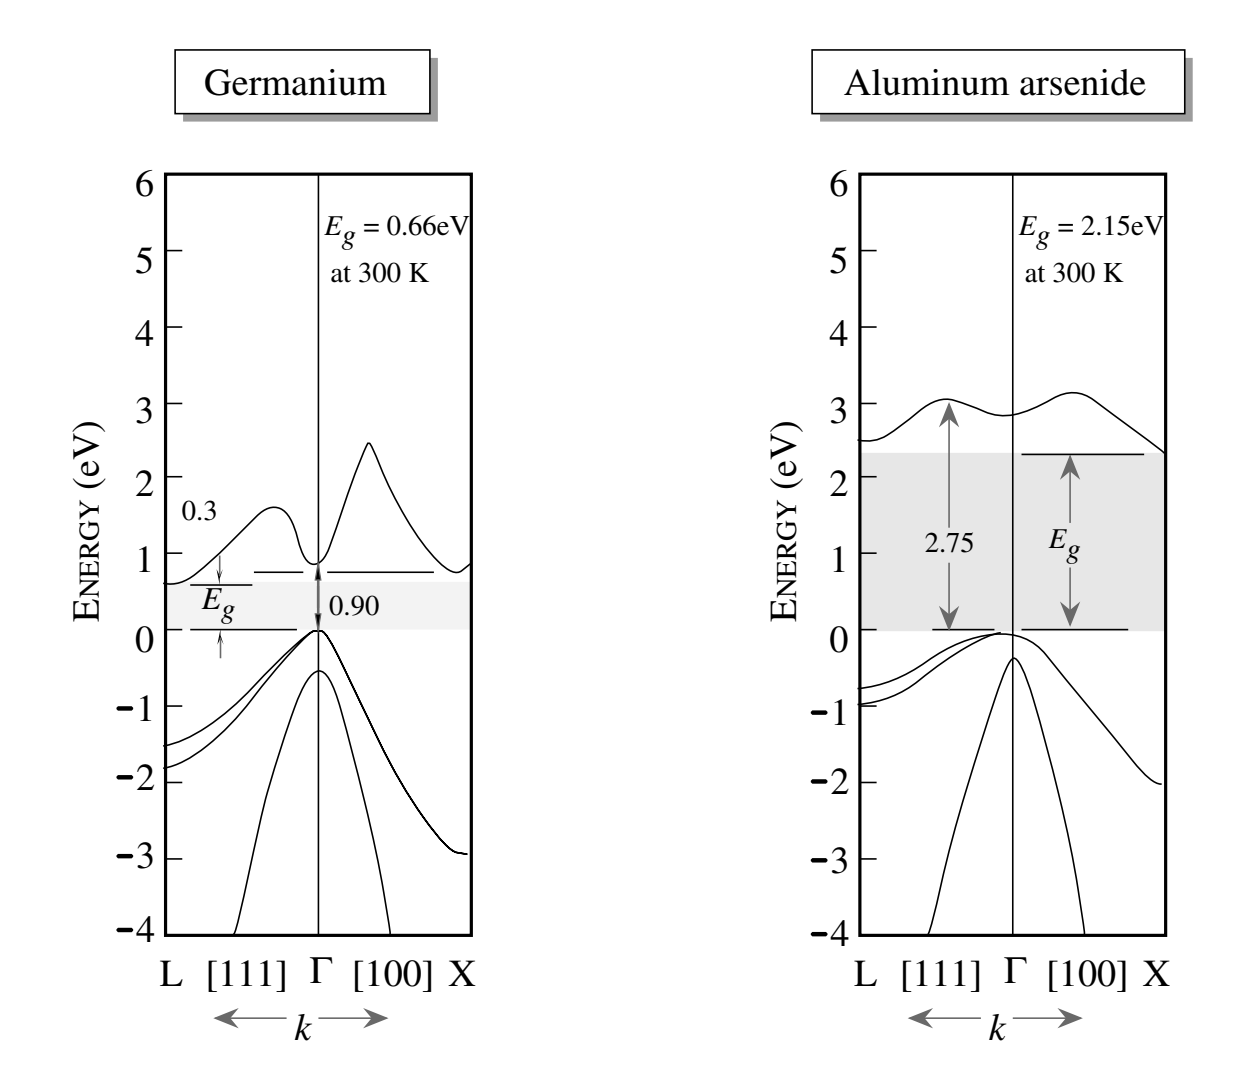
\includegraphics[width=\textwidth]{img/Germanium&Aluminium.png}
		\\[0.5em]
		\refstepcounter{figure}
		\textbf{Figure~\thefigure.}
		\label{fig:Germanium&Aluminium}
	\end{minipage}
\end{figure}

\begin{center}
	\begin{minipage}{0.7\textwidth}
		\centering
		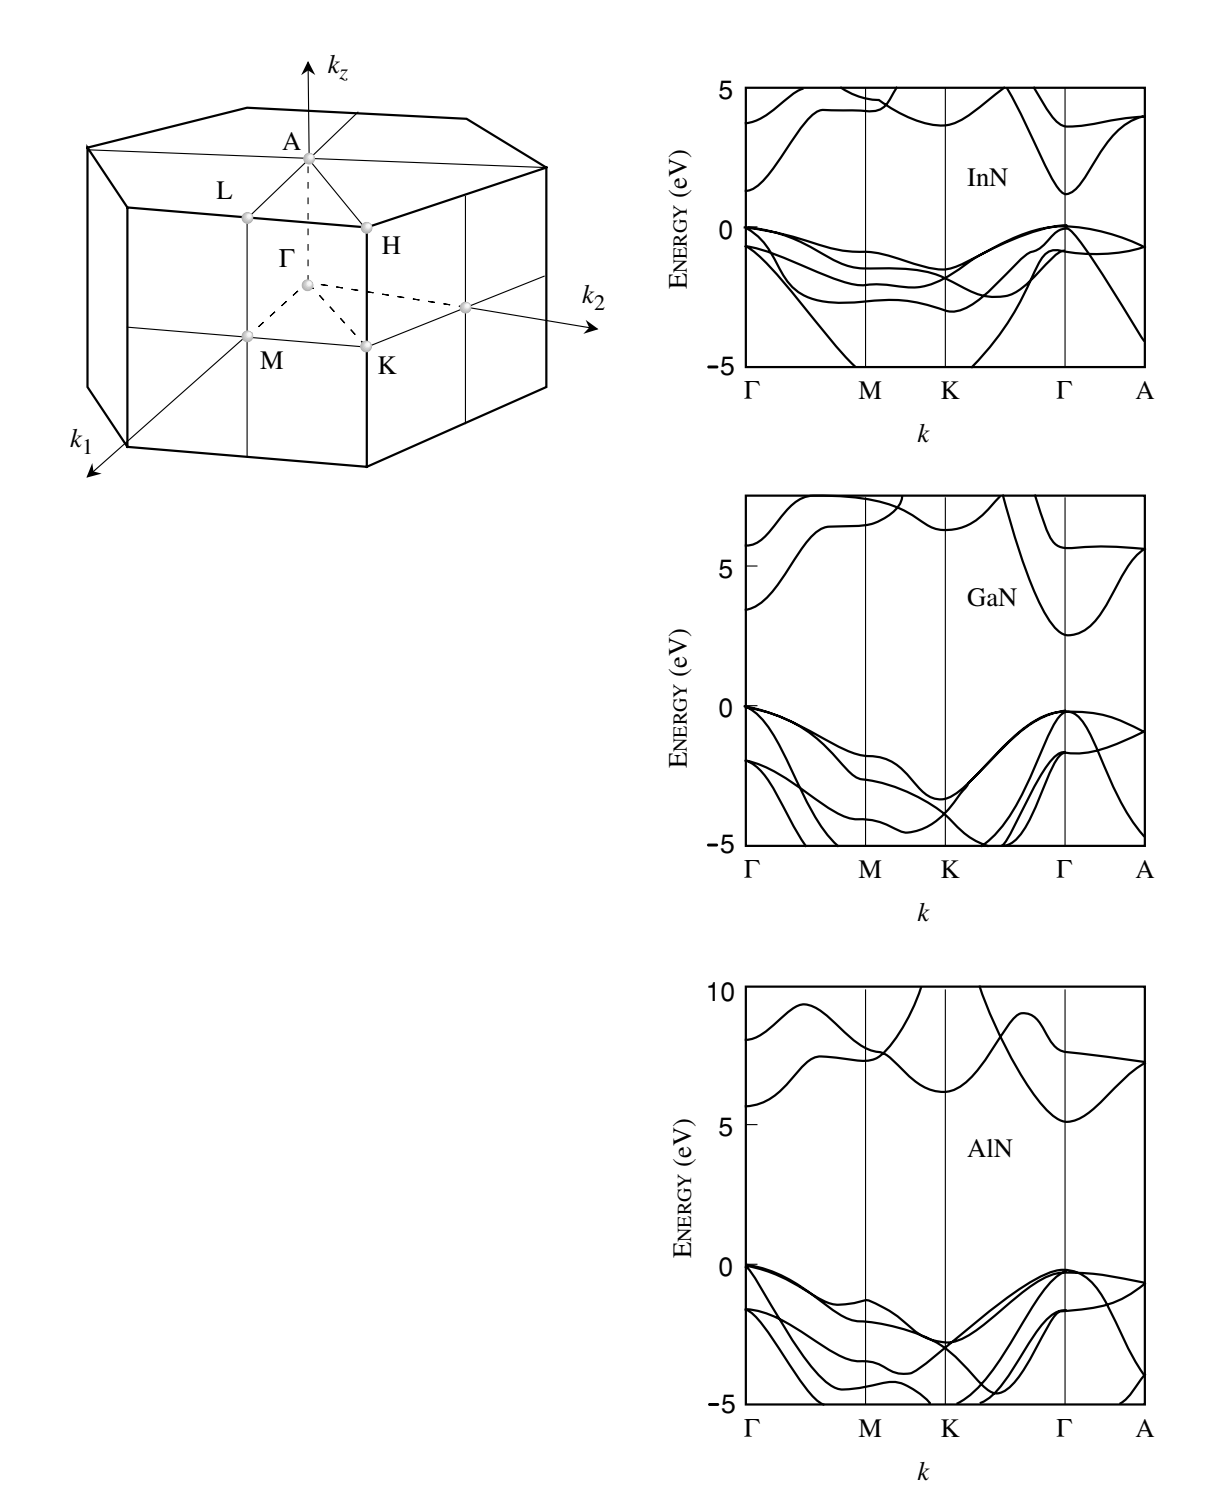
\includegraphics[width=\textwidth]{img/bandstructure_materials.png}
		\\[0.5em]
		\refstepcounter{figure}
		\textbf{Figure~\thefigure.}  Bandstructure of InN, GaN, and AlN. Also shown is the Brillioun zone.
		\label{fig:bandstructure_materials}
	\end{minipage}
\end{center}


\section{Mobile Carriers: Intrinsic Carriers}
In metals, the density of mobile charge carriers is extremely high, typically on the order of \( \sim 10^{23}~\text{cm}^{-3} \). In contrast, a semiconductor with a completely filled valence band and an empty conduction band does not conduct current under equilibrium conditions.

However, if electrons are excited from the valence band into the conduction band—either thermally or through doping—then two types of mobile charge carriers can exist. The electrons promoted to the conduction band contribute to conduction, and the absence of electrons (i.e., holes) left behind in the valence band also behave as positively charged mobile carriers.

If the concentration of conduction band electrons is denoted by \( n \), and the concentration of holes in the valence band is \( p \), then the total mobile carrier concentration in the material is given by:

\begin{equation}
	n_{\text{total}} = n + p
\end{equation}
In a three-dimensional semiconductor, the density of states (DOS) in the conduction band is given by:
\begin{equation}
	N(E) = \frac{\sqrt{2} \left( m^*_{\text{dos}} \right)^{3/2} \left( E - E_c \right)^{1/2}}{\pi^2 \hbar^3}
\end{equation}
\noindent
where:
\begin{itemize}
	\item \( N(E) \) is the density of available electronic states per unit volume per unit energy,
	\item \( m^*_{\text{dos}} \) is the effective density of states mass for the conduction band,
	\item \( E_c \) is the conduction band edge.
\end{itemize}

\begin{center}
	\begin{minipage}{0.8\textwidth}
		\centering
		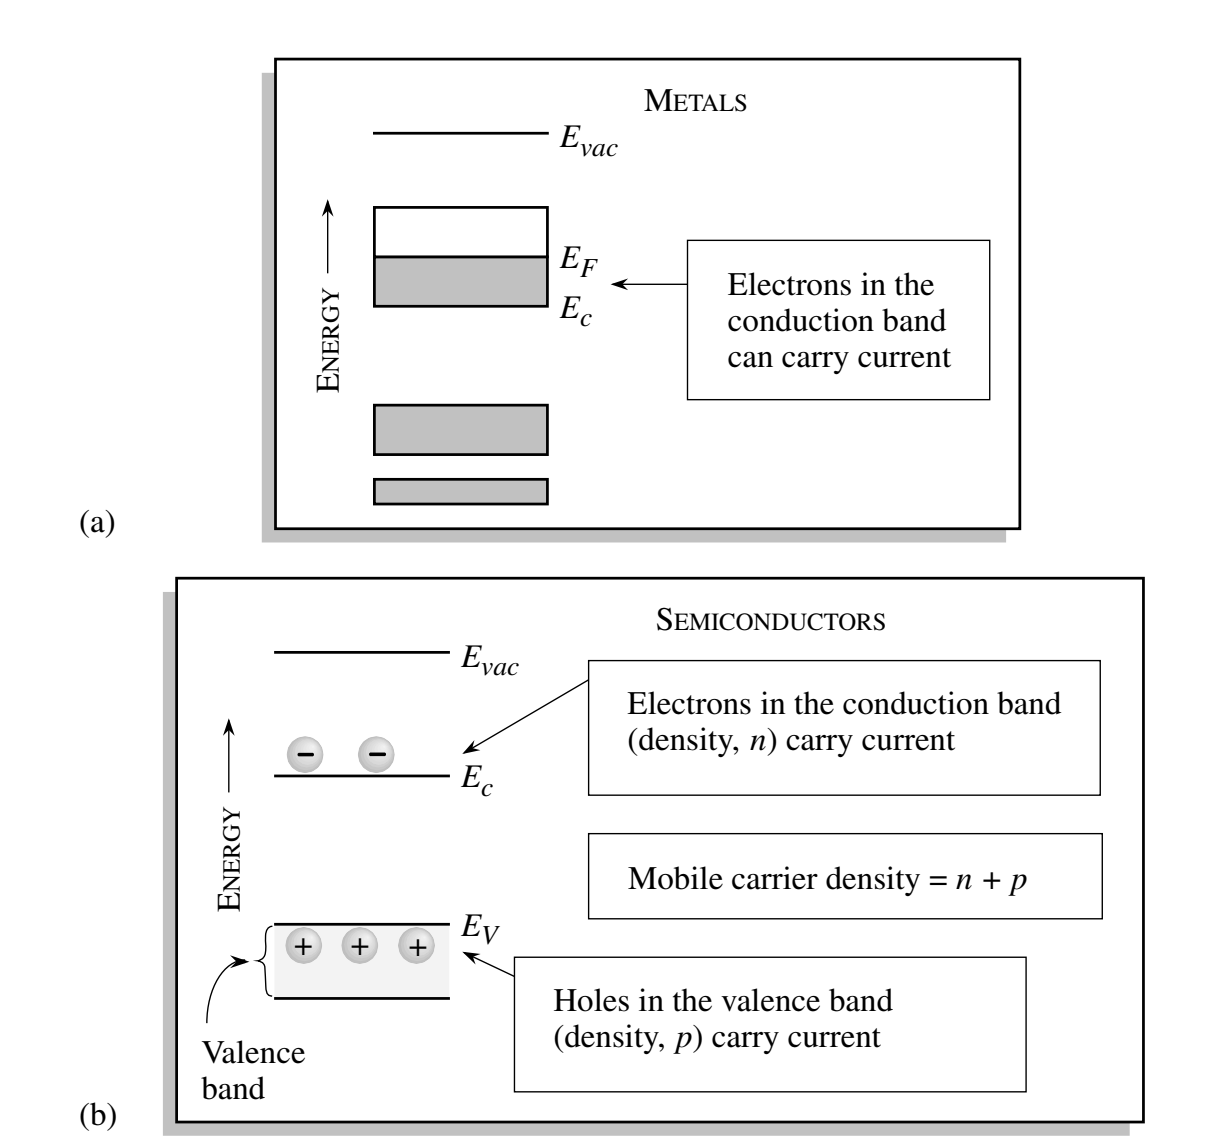
\includegraphics[width=\textwidth]{img/scheme_allowed_energy.png}
		\\[0.5em]
		\refstepcounter{figure}
		\textbf{Figure~\thefigure.}  (a) Schematic of allowed energy bands in a metal. Electrons in the highest partially filled band contribute to electrical conduction.
		(b) Energy band diagram of a typical semiconductor, where current is carried by electrons in the conduction band and holes in the valence band.
		\label{fig:allowed_energy_bands}
	\end{minipage}
\end{center}

In direct bandgap semiconductors, the density of states effective mass \( m^*_{\text{dos}} \) for the conduction band is simply equal to the electron effective mass at the band minimum. However, in indirect bandgap semiconductors, \( m^*_{\text{dos}} \) is defined as the geometric mean of the effective masses along the three principal axes:
\begin{equation}
	m^*_{\text{dos}} = \left( m_1^* m_2^* m_3^* \right)^{1/3}
\end{equation}
\noindent
where \( m_1^*, m_2^*, m_3^* \) are the effective masses along the principal crystallographic directions. For silicon, which has six equivalent \( X \)-valleys, this becomes:
\begin{equation}
	m^*_{\text{dos}} = 6 \left( m_t^2 m_l \right)^{1/3}
\end{equation}
\noindent
where \( m_l \) and \( m_t \) are the longitudinal and transverse effective masses of the conduction band ellipsoids, respectively.

For the valence band, which consists of heavy hole (HH) and light hole (LH) bands, the effective density of states mass can be approximated by:
\begin{equation}
	m^*_{\text{dos}} = \left( m_{\text{hh}}^{*3/2} + m_{\text{lh}}^{*3/2} \right)^{2/3}
\end{equation}

In intrinsic semiconductors, conduction band electrons originate from the valence band, and thus the electron and hole densities are equal:
\begin{equation*}
	n = p = n_i = p_i
\end{equation*}
The electron concentration in the conduction band is given by the integral:
\begin{equation}
	n = \int_{E_c}^{\infty} N_e(E) f(E) \, dE
\end{equation}
\noindent
Using the expression for the density of states and the Fermi-Dirac distribution, this becomes:
\begin{equation}
	n = \frac{1}{2\pi^2} \left( \frac{2 m_e^*}{\hbar^2} \right)^{3/2} \int_{E_c}^{\infty} \frac{(E - E_c)^{1/2}}{1 + \exp\left( \frac{E - E_F}{k_B T} \right)} \, dE
\end{equation}
\noindent
In the non-degenerate limit, where \( (E - E_F) \gg k_B T \), we can approximate the Fermi-Dirac function by the Boltzmann distribution, and the integral simplifies to:
\begin{equation}
	n = N_c \exp \left( \frac{E_F - E_c}{k_B T} \right)
\end{equation}
\noindent
where the effective density of states in the conduction band is:
\begin{equation}
	N_c = 2 \left( \frac{m_e^* k_B T}{2\pi \hbar^2} \right)^{3/2}
\end{equation}
A similar result holds for the hole concentration:
\begin{equation}
	p = N_v \exp \left( \frac{E_v - E_F}{k_B T} \right)
\end{equation}
\noindent
where:
\begin{equation}
	N_v = 2 \left( \frac{m_h^* k_B T}{2\pi \hbar^2} \right)^{3/2}
\end{equation}

The product \( np \) is independent of the Fermi level and depends only on temperature and intrinsic material properties:
\begin{equation}
	np = N_c N_v \exp \left( \frac{-E_g}{k_B T} \right)
\end{equation}
\noindent
This result is known as the \textit{law of mass action}. If \( n \) increases, \( p \) must decrease accordingly to maintain this constant product, and vice versa.

For an intrinsic semiconductor, where \( n = p = n_i \), we can express the intrinsic carrier concentration as:
\begin{equation}
	n_i = p_i = 2 \left( \frac{k_B T}{2\pi \hbar^2} \right)^{3/2} \left( m_e^* m_h^* \right)^{3/4} \exp \left( \frac{-E_g}{2k_B T} \right)
\end{equation}
Additionally, the intrinsic Fermi level \( E_i \) is approximately given by:
\begin{equation}
	E_i = \frac{E_c + E_v}{2} + \frac{3}{4} k_B T \ln \left( \frac{m_h^*}{m_e^*} \right)
\end{equation}
In computing the density of states masses \( m_e^* \) and \( m_h^* \), one must account for the number of equivalent conduction band valleys and the contributions from both heavy and light hole bands in the valence band.
\begin{center}
	\begin{minipage}{0.9\textwidth}
		\centering
		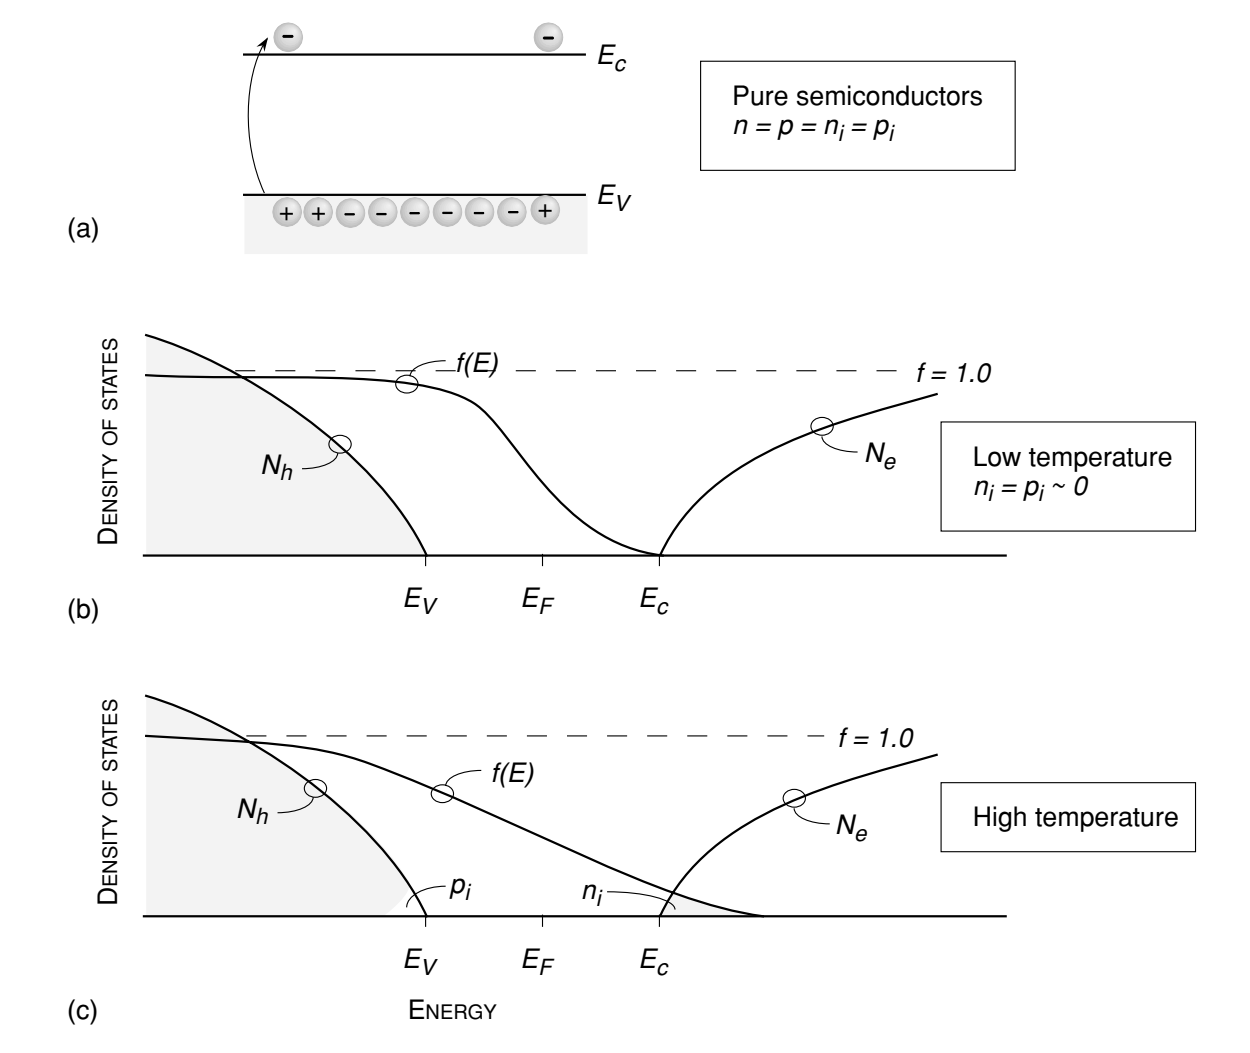
\includegraphics[width=\textwidth]{img/hole_denisties&Fermi_occupation.png}
		\\[0.5em]
		\refstepcounter{figure}
		\textbf{Figure~\thefigure.}
		(a) Illustration of equal electron and hole concentrations in an intrinsic (pure) semiconductor.
		(b) Density of states and Fermi-Dirac distribution at low temperature.
		(c) Density of states and Fermi function at high temperature, where intrinsic carrier concentrations $n_i$ and $p_i$ increase significantly.
		\label{fig:hole_denisties&Fermi_occupation}
	\end{minipage}
\end{center}

\section{Doping: Donors and Acceptors}
There are two primary types of dopants in semiconductors: \textit{donors}, which contribute electrons to the conduction band, and \textit{acceptors}, which accept electrons from the valence band, thereby creating holes. To understand how donor and acceptor states arise, consider a donor atom substituted into a crystal lattice.\\
For example, in silicon, a typical donor is a group V (pentavalent) atom that replaces a Si atom. Four of the donor's valence electrons form covalent bonds with neighboring Si atoms, just as in a normal Si lattice. The fifth valence electron, however, is left loosely bound. It experiences an attractive force from the now positively charged donor ion, which has a net charge of \( +e \). This interaction is Coulombic in nature but is screened by the dielectric constant \( \varepsilon \) of the semiconductor:
\begin{equation}
	U(r) = -\frac{e^2}{4\pi \varepsilon r}
\end{equation}
\noindent
where \( \varepsilon = \varepsilon_0 \varepsilon_r \), the product of vacuum permittivity and the relative dielectric constant of the material.\\
This scenario closely resembles the hydrogen atom problem, but with two modifications: the electron has an effective mass \( m^* \) rather than the free electron mass, and the Coulomb potential is reduced by the dielectric screening. The ground-state energy of the donor-bound electron is then given by:
\begin{equation}
	E_d = E_c - \frac{m^* e^4}{2(4\pi \varepsilon)^2 \hbar^2}
	= E_c - 13.6\,\text{eV} \left( \frac{m^*}{m_0} \right) \left( \frac{1}{\varepsilon_r^2} \right)
\end{equation}
\noindent
where \( E_c \) is the conduction band edge, and \( m_0 \) is the free electron mass.
In contrast to the hydrogen atom, where the energy level is referenced to the vacuum, in semiconductors, the donor energy is referenced from the conduction band edge. The effective mass \( m^* \) used in this calculation is the conductivity effective mass \( m^*_\sigma \), which reflects how electrons respond to external fields. This mass also governs donor binding energies and charge transport.\\
For direct bandgap semiconductors such as GaAs, the conductivity mass is simply the electron effective mass at the conduction band minimum. In indirect semiconductors like silicon, the conductivity mass is given by:
\begin{equation}
	{m^*_\sigma} = 3\left( \frac{1}{m_l^*} + \frac{2}{m_t^*} \right)^{-1}
\end{equation}
\noindent
where \( m_l^* \) and \( m_t^* \) are the longitudinal and transverse effective masses of the conduction band valleys.\\
\begin{figure}[h!]
	\centering
	\begin{minipage}{0.44\textwidth}
		\centering
		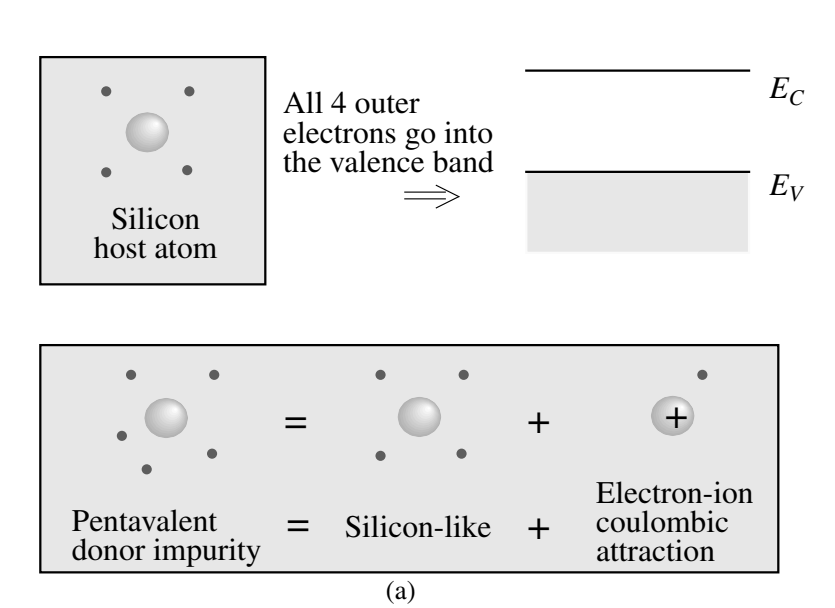
\includegraphics[width=\textwidth]{img/donors&acceptors.png}
		\\[0.5em]
		\refstepcounter{figure}
		\textbf{Figure~\thefigure.} \small Schematic illustrating the donor model in semiconductors. The problem is approached by considering the host atom plus a Coulomb interaction. Silicon contributes four valence electrons per atom. A donor atom provides five electrons, four of which fill the valence band, while the fifth can be thermally excited into the conduction band.
		\label{fig:donors&acceptors}
	\end{minipage}%
	\hfill
	\begin{minipage}{0.52\textwidth}
		\centering
		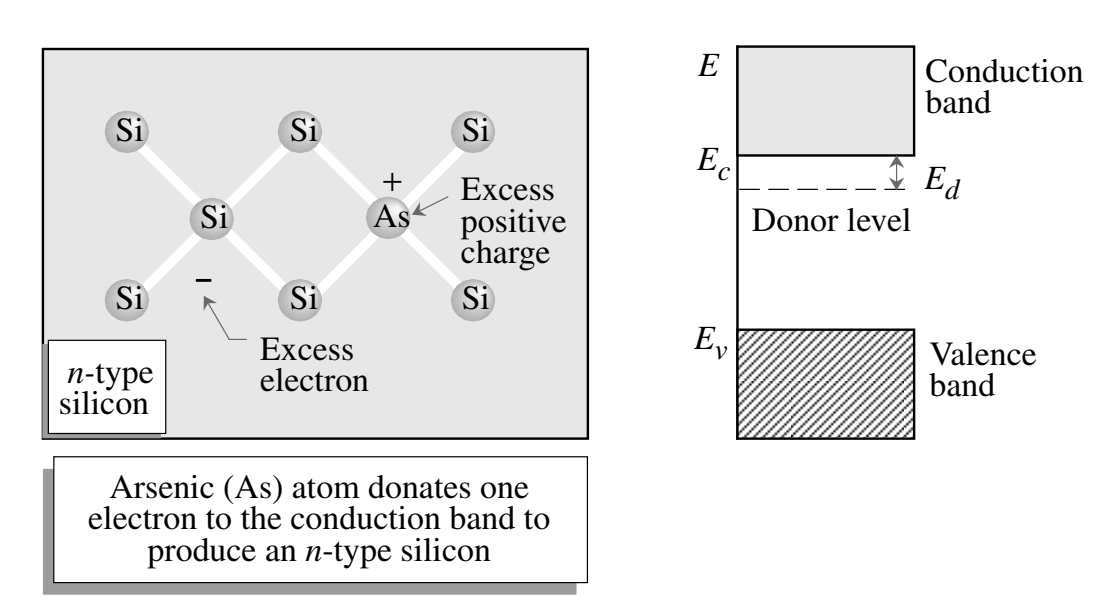
\includegraphics[width=\textwidth]{img/SiAs.png}
		\\[0.5em]
		\refstepcounter{figure}
		\textbf{Figure~\thefigure.} \small Charge distribution around an arsenic impurity in silicon. Arsenic, with five valence electrons, forms four covalent bonds like silicon, while the fifth electron remains free for conduction. Upon ionization, the arsenic atom donates this electron to the conduction band and acts as a donor.
		\label{fig:SiAs}
	\end{minipage}
\end{figure}
According to this simplified model, the donor binding energy depends only on the properties of the host material—namely, its dielectric constant \( \varepsilon_r \) and effective mass \( m^* \)—and not on the specific dopant species. Using this model, typical donor binding energies are:
\begin{itemize}
	\item Germanium (Ge): \( \sim 0.006\,\text{eV} \)
	\item Silicon (Si): \( \sim 0.025\,\text{eV} \)
	\item Gallium Arsenide (GaAs): \( \sim 0.007\,\text{eV} \)
\end{itemize}
In practice, small deviations from these values occur due to simplifications in the model. The discrepancy arises from local modifications in the potential near the impurity site—known as the \textit{central cell correction}—which slightly perturbs the donor energy levels beyond what is predicted by the hydrogenic approximation.\\
Acceptors represent another class of intentional impurities. Like donors, they introduce localized energy levels in the bandgap. An acceptor is neutral when unoccupied and negatively charged when it captures an electron from the valence band, leaving behind a mobile hole. These levels are created by substituting host atoms with impurities that have one fewer valence electron. For example, group III elements act as acceptors in group IV semiconductors such as Si and Ge, while Si can act as an acceptor in GaAs if it replaces an As atom.\\
Thus, donors and acceptors serve to modulate the free carrier concentrations in semiconductors, enabling control over electronic and optoelectronic behavior.

\subsection{Carriers in Doped Semiconductors}
As previously discussed, introducing a donor atom into a semiconductor can, in principle, contribute an extra electron to the conduction band. However, whether this electron becomes a free carrier or remains bound to the donor site depends on several factors: the donor binding energy, the donor concentration, and the temperature.\\
At very low temperatures, donor electrons typically remain bound to their parent atoms. This phenomenon, known as \textit{carrier freezeout}, results in minimal free carrier concentration and hence poor conductivity. As the temperature increases, thermal energy becomes sufficient to ionize donor electrons, which then occupy states in the conduction band and act as mobile charge carriers. These free electrons significantly affect the electrical conductivity of the material. The donor site, now lacking an electron, becomes a positively charged ion.\\
A similar process occurs for acceptor atoms: when an acceptor captures an electron from the valence band, it becomes negatively charged and creates a mobile hole in the valence band.\\
In general, as discussed before, the relationship between the electron concentration \( n \) and the Fermi level \( E_F \) is given by:
\begin{equation*}
	n = \int_{E_c}^\infty N(E) f(E) \, dE
\end{equation*}
\noindent
This equation must usually be solved numerically. However, a useful analytical approximation is provided by the \textit{Joyce–Dixon} formula. According to this approximation, the Fermi level is related to the carrier concentration as follows:
\begin{equation}
	E_F = E_c + k_B T \ln \left( \frac{n}{N_c} \right) + \frac{k_B T}{\sqrt{8}} \left( \frac{n}{N_c} \right)
\end{equation}
\noindent
Alternatively, for hole concentration \( p \), the expression becomes:
\begin{equation}
	E_F = E_v - k_B T \ln \left( \frac{p}{N_v} \right) - \frac{k_B T}{\sqrt{8}} \left( \frac{p}{N_v} \right)
\end{equation}
\noindent
The effective density of states in the conduction band is given by:
\begin{equation*}
	N_c = 2 \left( \frac{m_e^* k_B T}{2\pi \hbar^2} \right)^{3/2}
\end{equation*}
\noindent
and similarly, the valence band effective density of states is:
\begin{equation*}
	N_v = 2 \left( \frac{m_h^* k_B T}{2\pi \hbar^2} \right)^{3/2}
\end{equation*}
These expressions allow one to estimate the Fermi level \( E_F \) for a known carrier concentration \( n \), or vice versa, by iterative methods. If the correction terms \( (n/\sqrt{8}N_c) \) or \( (p/\sqrt{8}N_v) \) are neglected, the equations reduce to the standard Boltzmann approximation:
\begin{equation}
	n \approx N_c \exp \left( \frac{E_F - E_c}{k_B T} \right)
\end{equation}
\noindent
and
\begin{equation}
	p \approx N_v \exp \left( \frac{E_v - E_F}{k_B T} \right)
\end{equation}
This simplified form is valid under non-degenerate conditions, where the Fermi level is several \( k_B T \) away from the band edges.

\subsection{Mobile Carrier Density and Carrier Freezeout}
\begin{center}
	\begin{minipage}{0.7\textwidth}
		\centering
		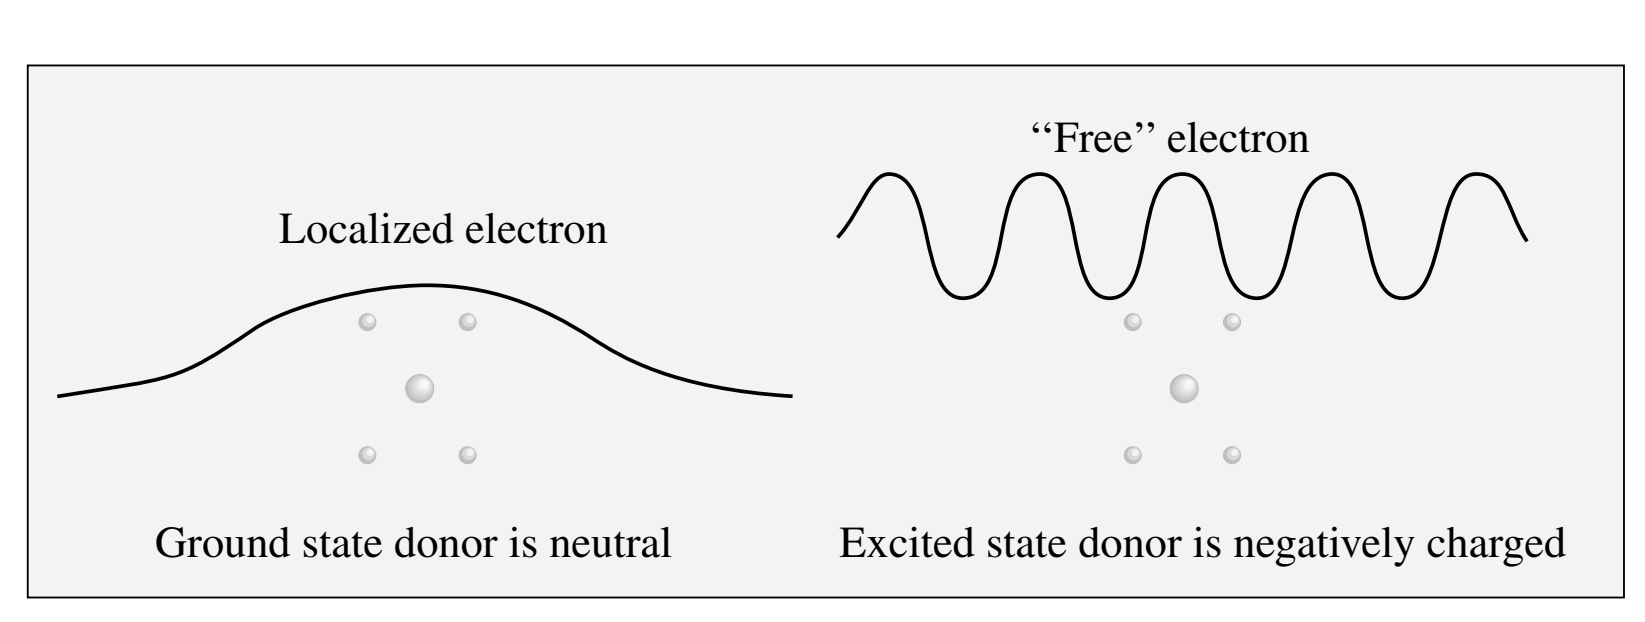
\includegraphics[width=\textwidth]{img/Electron_band.png}
		\\[0.5em]
		\refstepcounter{figure}
		\textbf{Figure~\thefigure.}An electron bound to a donor does not participate in conduction. Only when the donor is ionized does the electron become free and contribute to electrical transport.
		\label{fig:Electron_band}
	\end{minipage}
\end{center}

In the ground state of a donor atom embedded in a semiconductor, the excess electron introduced by the donor is localized near the donor nucleus. Since this bound state does not contribute to electrical conductivity, such electrons are not useful for modifying the electronic properties of the material.\\
At very low temperatures, donor electrons remain bound to the donor atoms—a phenomenon known as \textit{carrier freeze-out}. As the temperature increases, thermal excitation allows the donor electrons to be ionized into the conduction band, where they become mobile and contribute to current transport. The donor atom, once ionized, becomes positively charged and acts as a scattering center for conduction electrons. The detailed analysis of scattering effects will be addressed in a later section.\\
The electron–donor system may exist in the following possible configurations:
\begin{enumerate}
	\item the donor electron is ionized and free in the conduction band;
	\item one electron is bound to the donor atom (with spin-up or spin-down);
	\item two electrons attempt to occupy the donor site.
\end{enumerate}
Although the third case is theoretically possible, the strong Coulombic repulsion between two electrons on the same donor site makes such double occupation energetically prohibitive. Therefore, a donor can bind at most one electron at a time, with either spin orientation.\\
Due to the two available spin states for the bound electron, the donor occupation statistics follow Fermi–Dirac statistics with a factor of two in the numerator. The probability that a donor level at energy \( E_d \) is occupied by an electron is given by:
\begin{equation}
	f_d = \frac{1}{1 + \frac{1}{2} \exp\left( \frac{E_d - E_F}{k_B T} \right)}
\end{equation}
\noindent
where \( E_F \) is the Fermi level, \( k_B \) is Boltzmann’s constant, and \( T \) is the temperature.
The number density of electrons bound to donor sites is therefore:
\begin{equation}
	n_d = N_d \cdot f_d = \frac{N_d}{1 + \frac{1}{2} \exp\left( \frac{E_d - E_F}{k_B T} \right)}
\end{equation}
\noindent
For \( (E_d - E_F) \gg k_B T \), this simplifies to the Boltzmann approximation:
\begin{equation}
	n_d \approx 2 N_d \exp\left( -\frac{E_d - E_F}{k_B T} \right)
\end{equation}
Similarly, for acceptor levels, the probability that a hole is trapped at an acceptor level is given by:
\begin{equation}
	p_a = \frac{N_a}{1 + \frac{1}{4} \exp\left( \frac{E_F - E_a}{k_B T} \right)}
\end{equation}
\noindent
Here, \( E_a \) is the acceptor level energy, and the factor of \( \frac{1}{4} \) arises from the four-fold degeneracy associated with the doubly degenerate valence band and spin.\\
These expressions allow us to estimate the ionization state of donor and acceptor levels as a function of temperature and Fermi energy.


\subsection{Equilibrium Density of Carriers in Doped Semiconductors}
In a doped semiconductor, we may introduce donor atoms, acceptor atoms, or both. To determine the electron and hole concentrations under such conditions, we must consider the occupation functions of free carriers and dopant states. The key constraint that must be satisfied is the \textit{charge neutrality condition}, given by:
\begin{equation}
	n_c + n_d = N_d - N_a + p_v + p_a
\end{equation}
\noindent
where:
\begin{itemize}
	\item \( n_c \) is the density of free electrons in the conduction band,
	\item \( n_d \) is the density of electrons bound to donor atoms,
	\item \( p_v \) is the density of free holes in the valence band,
	\item \( p_a \) is the density of holes bound to acceptor atoms.
\end{itemize}
\noindent
The electron and hole densities depend on the Fermi energy \( E_F \), and hence the neutrality condition, combined with the Fermi–Dirac occupation probabilities, allows us to determine \( E_F \) at a given temperature. In the general case, this requires numerical methods: a trial Fermi level is chosen and adjusted iteratively until the neutrality equation is satisfied.\\
However, in the case of low doping levels—where carrier concentrations are small—the Boltzmann approximation can be applied, allowing for an analytical treatment. Under this approximation, and neglecting the unity in the denominator of the Fermi function, the free electron concentration is given by:
\begin{equation}
	n = N_c \exp\left( -\frac{E_c - E_F}{k_B T} \right)
\end{equation}
\noindent
For electrons bound to donors, we have:
\begin{equation}
	n_d = \frac{N_d}{1 + \frac{1}{2} \exp\left( \frac{E_d - E_F}{k_B T} \right)} \approx \frac{N_d}{2} \exp\left( \frac{E_d - E_F}{k_B T} \right)
\end{equation}
\noindent
Combining these, the total electron concentration becomes:
\begin{equation}
	n = n + n_d = N_c \exp\left( -\frac{E_c - E_F}{k_B T} \right) + \frac{N_d}{2} \exp\left(\frac{E_d - E_F}{k_B T} \right)
\end{equation}
\noindent
Alternatively, this can be rearranged as:
\begin{equation}
	\frac{n_d}{n_d + n_c} = \frac{1}{1 + \frac{N_c}{2 N_d} \exp\left( -\frac{E_c - E_d}{k_B T} \right)}
\end{equation}
For acceptor doping, a similar analysis leads to:
\begin{equation}
	\frac{p_a}{p + p_a} = \frac{1}{1 + \frac{N_v}{4N_a} \exp\left( -\frac{E_a - E_v}{k_B T} \right)}
\end{equation}
\noindent
where:
\begin{itemize}
	\item \( N_c \), \( N_v \) are the effective density of states in the conduction and valence bands, respectively,
	\item \( N_d \), \( N_a \) are the donor and acceptor concentrations,
	\item \( E_c \), \( E_v \), \( E_d \), and \( E_a \) are the band edge and dopant energy levels.
\end{itemize}
These relations provide a way to estimate carrier concentrations and dopant ionization under low doping conditions.

In the Fig.\ref{fig:Electron_band} we show how free electron density varies with temperature in a n-type silicon sample. As temperature increases, the fraction of “ionized” donors starts to increase until all of the donors are ionized and the free carrier density is equal to the donor density. This region is called the saturation region. Eventually, as the temperature is further raised, the carrier density starts to increase because of the intrinsic carrier density exceeding the donor density. At low temperatures the electrons are bound to the donors. This is the freezeout regime. Semiconductor devices usually operate in the satu- ration region where the mobile carrier density is essentially independent of temperature and is approximately equal to the doping density.
Semiconductor devices cannot operate in the high temperature intrinsic regime, since it is not possible to control intrinsic carrier density by applying an external bias. Thus devices cannot be “shut off ” due to the leakage current from intrinsic carriers. High temperature electronics require large bandgap semiconductors for which the upper temperature limit is high.

\subsection{Heavily Doped Semiconductors}
In the theory discussed so far, we have made several important assumptions that are valid only under low doping conditions:
\begin{enumerate}
	\item The bandstructure of the host crystal is assumed to remain unperturbed, such that the bandedge states are still well described by simple parabolic bands.
	\item Dopants are treated as isolated and non-interacting, with their potential modeled as a simple Coulombic potential.
\end{enumerate}
\noindent These assumptions break down as the doping level increases. When the average spacing between impurity atoms becomes comparable to $\sim 100$~\AA, the potential experienced by an impurity electron is significantly influenced by neighboring impurities. This situation is analogous to the transition from isolated atomic levels to energy bands in a crystal. When atoms are far apart, discrete energy levels exist; however, as their separation decreases to a few angstroms, these levels broaden into bands due to interatomic interactions.\\
\noindent Similarly, at high doping levels, impurity states can overlap and form \textit{impurity bands}. In this regime, several additional physical effects arise, altering the electrical and optical properties of the semiconductor. These effects must be considered for a proper understanding of heavily doped semiconductors.

\chapter{Bandstructure Modifications}

\section{Bandstructure of Semiconductor Alloys}
One of the simplest and most effective methods to alter the electronic properties of a material or to engineer entirely new properties is through the formation of alloys. Alloying has long been employed across various material classes—not only semiconductors, but also metals and insulators—as a technique to tailor physical and chemical characteristics.

In the context of semiconductors, the motivation to create alloys is typically driven by two primary goals:

\begin{enumerate}
	\item \textit{Tuning the bandgap}: This is particularly important in the design of light-emitting and light-detecting devices, where the bandgap dictates the energy (and thus the wavelength) of the absorbed or emitted photons.
	\item \textit{Lattice constant engineering}: Alloying allows for the synthesis of materials with desired lattice parameters, enabling lattice matching (or deliberate mismatch) with available substrates. For instance, the InGaAs alloy is frequently used because it can be lattice-matched to InP substrates, which are commercially available.
\end{enumerate}
\begin{center}
	\begin{minipage}{0.7\textwidth}
		\centering
		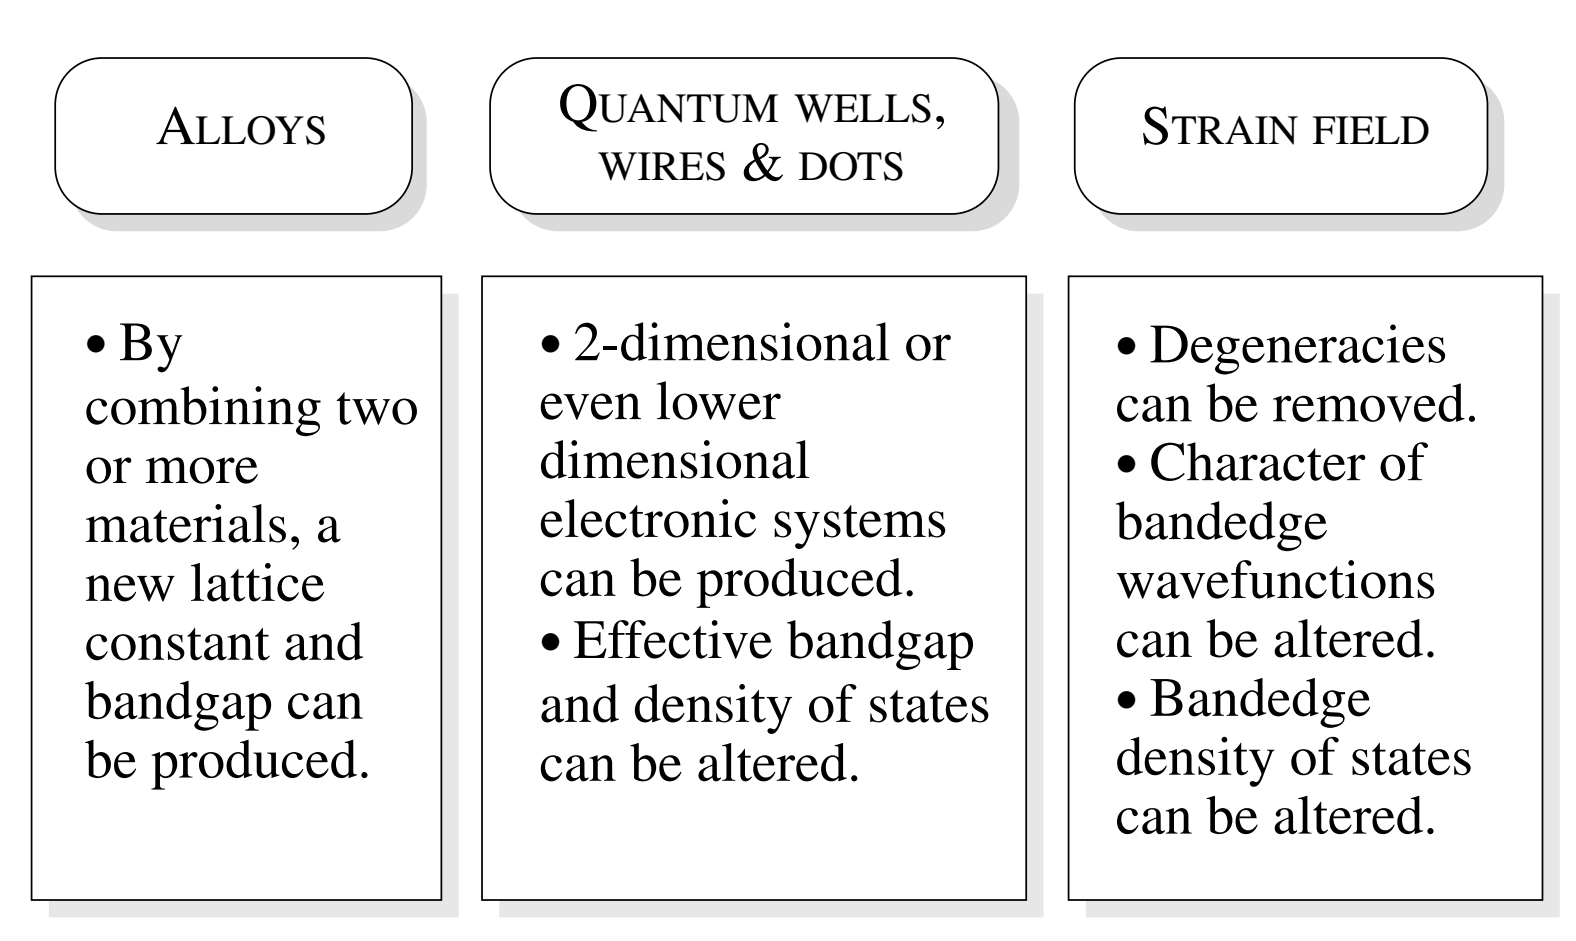
\includegraphics[width=\textwidth]{img/Approaches_BandStructureMod.png}
		\\[0.5em]
		\refstepcounter{figure}
		\textbf{Figure~\thefigure.} Different approaches to modify Bandstructure of semiconductors.
		\label{fig:Approaches_BandStructureMod}
	\end{minipage}
\end{center}
When an alloy of the form \( A_{x}B_{1-x} \) is produced via random mixing of two components \( A \) and \( B \) (a concept that can be generalized to multicomponent systems), the lattice constant of the resulting alloy is often estimated using Vegard's law:
\[
	a_{\text{alloy}} = x a_A + (1 - x) a_B
\]
This empirical relationship assumes a linear interpolation between the lattice constants \( a_A \) and \( a_B \) of the pure materials and is valid for random alloys where no phase separation occurs and both components share the same crystal structure.
The term "random" in this context refers to the statistical distribution of atoms within the alloy. Specifically, in a random alloy, the probability that a given atomic site is occupied by atom \( A \) is \( x \), while the probability that it is occupied by atom \( B \) is \( 1 - x \). However, several distinct atomic arrangements are theoretically possible when forming such an alloy:
\begin{enumerate}
	\item \textit{Phase separation}: Atoms of type \( A \) cluster together in one region, while atoms of type \( B \) cluster in another, forming distinct domains of the pure components.
	\item \textit{Random distribution}: Each atomic site is occupied according to the probability \( x \) for \( A \) and \( 1 - x \) for \( B \), independent of neighboring sites.
	\item \textit{Ordered structure}: Atoms \( A \) and \( B \) arrange themselves in a well-defined periodic pattern, forming a superlattice.
\end{enumerate}
\begin{center}
	\begin{minipage}{0.4\textwidth}
		\centering
		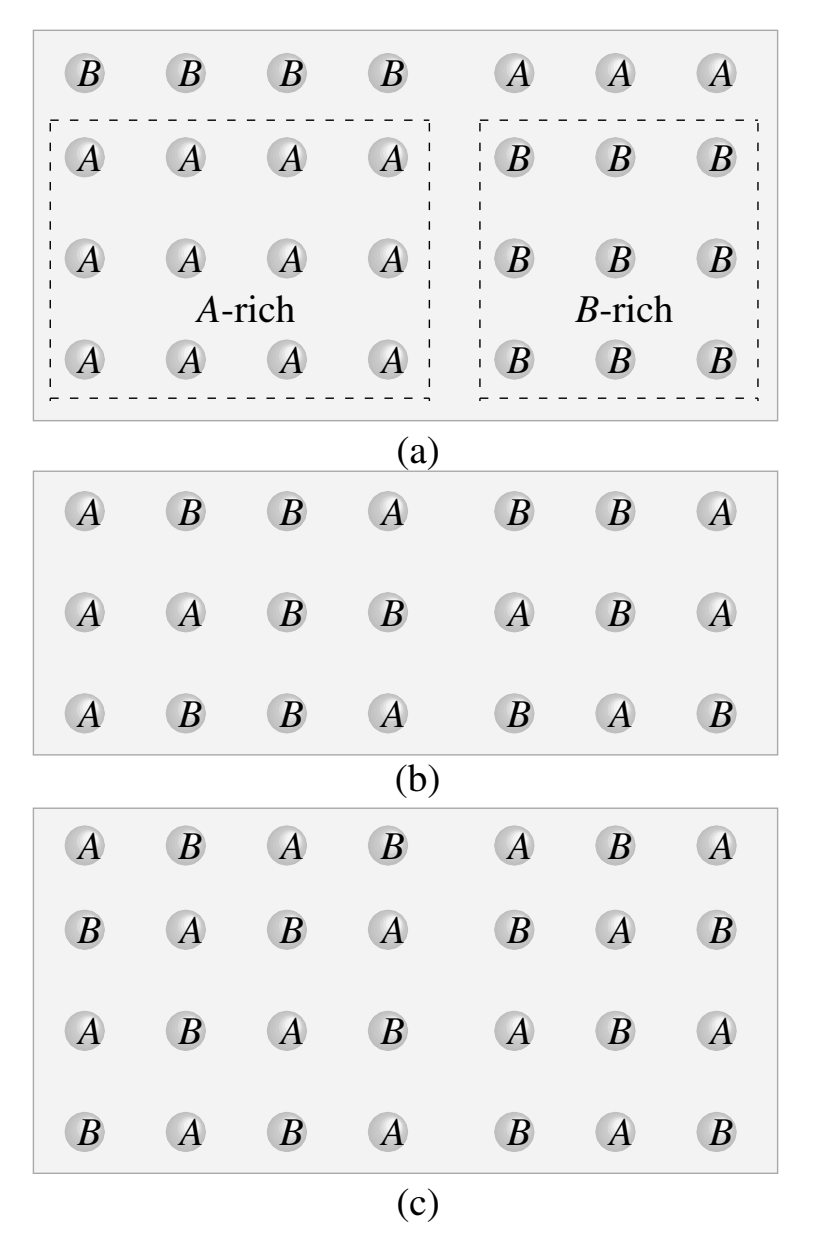
\includegraphics[width=\textwidth]{img/clustered-ordered-ordered.png}
		\\[0.5em]
		\refstepcounter{figure}
		\textbf{Figure~\thefigure.} A schematic example of (a) a clustered, (b) a random, and (c) an ordered alloy structure.
		\label{fig:clustered-ordered-ordered}
	\end{minipage}
\end{center}

In practice, most semiconductor alloys used in modern electronic and optoelectronic applications are synthesized with the goal of producing statistically random distributions of constituent atoms. Such random alloys provide the desired combination of bandgap tunability and structural compatibility with various substrates.\\
Alloys typically retain a well-defined crystal structure; however, the random occupation of lattice sites by different atomic species eliminates the strict periodicity of the background potential—except in the case of ordered alloys or superlattices. As a result, Bloch’s theorem no longer applies, and the electronic wavefunctions can no longer be represented as simple traveling waves. Instead, they become more complex, exhibiting spatially varying probability distributions.
To make progress in understanding the bandstructure of such disordered systems, a commonly employed approximation is the \textit{virtual crystal approximation} (VCA). This approach replaces the spatially random potential experienced by the electrons with an averaged periodic potential:
\begin{equation}
	U_{\text{av}}(\mathbf{r}) = x U_A(\mathbf{r}) + (1 - x) U_B(\mathbf{r})
\end{equation}
Here, \( U_A \) and \( U_B \) are the atomic potentials of the two constituent species, and \( x \) represents the concentration of species \( B \). The VCA allows one to treat the alloy as if it were a periodic crystal with an effective potential.
In practical implementations—such as within the tight-binding method—this corresponds to averaging the matrix elements of the Hamiltonian. For direct bandgap semiconductors, where the conduction and valence band edges occur at the \(\Gamma\)-point (i.e., \( \mathbf{k} = 0 \)), the bandgap is also approximated by a linear interpolation:
\begin{equation}
	E_g^{\text{alloy}} = x E_g^A + (1 - x) E_g^B
\end{equation}
However, in many real materials, this linear relationship is not sufficient due to a phenomenon known as \textit{bandgap bowing}. This deviation arises from the increasing disorder and complex interactions introduced by alloying. A more accurate empirical expression for the bandgap is:
\begin{equation}
	E_g^{\text{alloy}} = a + bx + c x^2
\end{equation}
where \( a \), \( b \), and \( c \) are material-specific constants, and \( c \) is known as the bowing parameter.
In addition to bandgap behavior, the effective masses at the band edges also vary with composition. Within the VCA, the effective mass of the alloy can be approximated by:
\begin{equation}
	\frac{1}{m^*_{\text{alloy}}} = \frac{x}{m^*_A} + \frac{1 - x}{m^*_B}
\end{equation}
This follows from the expression for the energy dispersion near the band edge, assuming parabolic bands:
\begin{equation}
	E_{\text{alloy}}(k) = x \frac{\hbar^2 k^2}{2 m^*_A} + (1 - x) \frac{\hbar^2 k^2}{2 m^*_B}
\end{equation}
Several important alloy systems have played critical roles in advancing semiconductor electronics and optoelectronics. These will be briefly discussed in the following sections.
\begin{center}
	\begin{minipage}{0.9\textwidth}
		\centering
		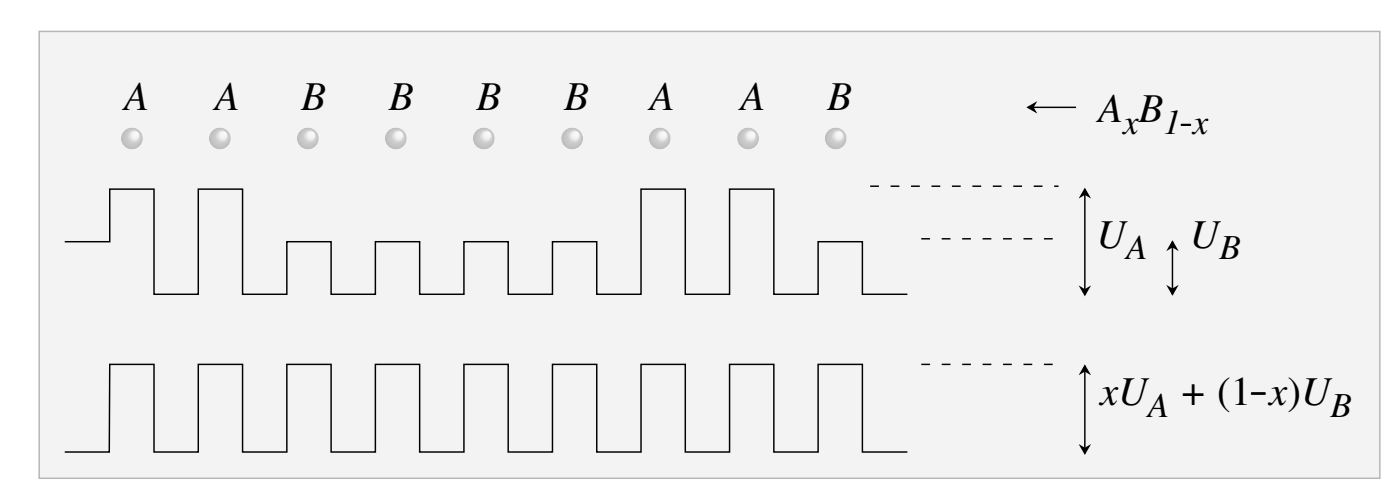
\includegraphics[width=\textwidth]{img/VCA.png}
		\\[0.5em]
		\refstepcounter{figure}
		\textbf{Figure~\thefigure.} Motivation for the virtual crystal approximation (VCA). The top part illustrates a lattice with A- and B-type atoms, each associated with localized potentials $U_A$ and $U_B$. In the VCA, extended states experience an effective periodic potential given by the weighted average $xU_A + (1 - x)U_B$.
		\label{fig:VCA}
	\end{minipage}
\end{center}

\subsection{GaAs/AlAs Alloy}
The AlGaAs system is among the most important and widely studied semiconductor alloy systems. A key advantage of this system is that AlAs and GaAs are nearly lattice matched, allowing the alloy \( \text{Al}_x\text{Ga}_{1-x}\text{As} \) to be epitaxially grown on GaAs substrates without the buildup of significant strain energy. This lattice compatibility makes AlGaAs highly suitable for the fabrication of high-speed electronic and optoelectronic devices.\\
In electronic applications, AlGaAs plays a central role in the development of modulation-doped field-effect transistors (MODFETs), while in optoelectronics it is used in a variety of devices such as modulators, photodetectors, and laser diodes.\\
One particularly noteworthy property of the AlGaAs alloy system is the compositional dependence of its electronic band structure, specifically the nature of its bandgap. As the aluminum content increases, the conduction band minimum transitions from the \(\Gamma\)-valley to the \(X\)-valley, resulting in a switch from a direct to an indirect bandgap.\\
This transition typically occurs when the aluminum mole fraction exceeds approximately 35\%. Consequently, for most optoelectronic device applications that require efficient radiative recombination (i.e., direct bandgap), the aluminum composition is chosen to be below this threshold.\\
This compositional dependence of the conduction band valleys is critical in determining the optical and electronic properties of AlGaAs-based devices and must be carefully accounted for in device design and material synthesis.
\begin{center}
	\begin{minipage}{0.7\textwidth}
		\centering
		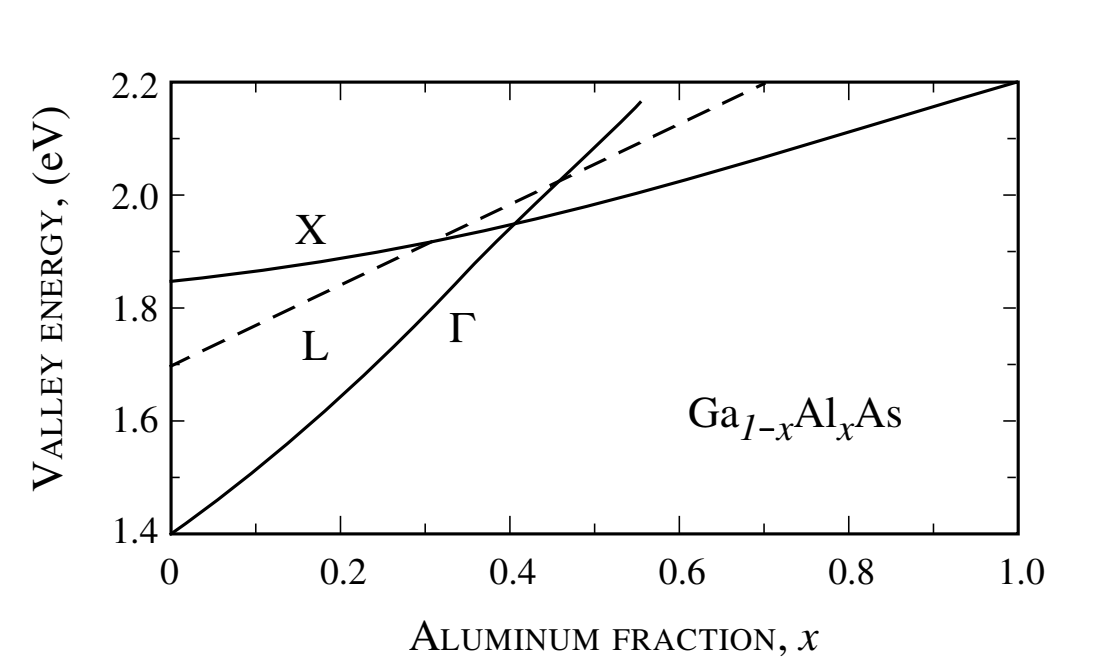
\includegraphics[width=\textwidth]{img/AlGaAs.png}
		\\[0.5em]
		\refstepcounter{figure}
		\textbf{Figure~\thefigure.} The variation of conduction band valleys in AlGaAs as a function of composition at 300 K.
		\label{fig:AlGaAs}
	\end{minipage}
\end{center}

\section{Bandstructure Modifications by Heterostructures}
It is possible to vary the chemical composition of a semiconductor structure along the growth direction using advanced epitaxial techniques such as molecular beam epitaxy (MBE) or metal-organic chemical vapor deposition (MOCVD). By introducing compositionally distinct layers, one can fabricate heterostructures capable of confining electronic states, thereby creating lower-dimensional systems. These systems are now widely utilized in high-performance optoelectronic and electronic devices.\\
Considerable effort has been devoted to extending confinement from one dimension (quantum wells) to two-dimensional (quantum wires) and three-dimensional (quantum dots) systems. While confinement in one dimension is conceptually straightforward and technologically mature, achieving confinement in additional directions often requires complex and challenging epitaxial or post-growth processing techniques.\\
As previously discussed, strained epitaxy can lead to the formation of self-assembled quantum dots, which serve as quasi-zero-dimensional (0D) systems. These have enabled the development of novel device architectures. Although our focus will remain primarily on quantum wells, we will also highlight key considerations related to quantum dots.\\
When two semiconductors are joined to form a heterostructure, one of the most critical questions is how the band edges of the two materials align at the interface. Suppose material \( A \) has a bandgap \( E_g^A \), conduction band edge \( E_c^A \), and valence band edge \( E_v^A \), and material \( B \) has a bandgap \( E_g^B \), with corresponding band edges \( E_c^B \) and \( E_v^B \). Several distinct band alignments may arise depending on the specific materials used.\\
In semiconductor physics, it is common to use electron affinity (or work function) to estimate how the conduction or valence bands align. However, this approach often fails for real heterojunctions due to complex interfacial effects such as charge transfer and atomic bonding. As a result, accurate determination of band lineups usually relies on experimental measurements, though theoretical predictions can often capture general trends.
Three main types of band alignments are typically observed:
\begin{itemize}
	\item \textbf{Type I (Straddling gap):} Both the conduction band minimum and valence band maximum of the narrower-gap material lie within the bandgap of the wider-gap material. This allows both electrons and holes to be confined in the same region. Common examples include GaAs/AlGaAs, InGaAs/InP, and GaN/AlGaN systems.
	\item \textbf{Type II (Staggered gap):} The conduction band minimum lies in one material while the valence band maximum lies in the other. Although this configuration may lead to a small effective bandgap, the spatial separation of carriers weakens optical transitions. Antimonide-based systems such as InSb and GaSb often exhibit type II alignment. The InAs/GaSb system is a well-known example.
	\item \textbf{Broken gap:} In some cases, the conduction band of one material lies below the valence band of the other. These are sometimes referred to as broken gap type II heterostructures.
\end{itemize}
\begin{center}
	\begin{minipage}{0.8\textwidth}
		\centering
		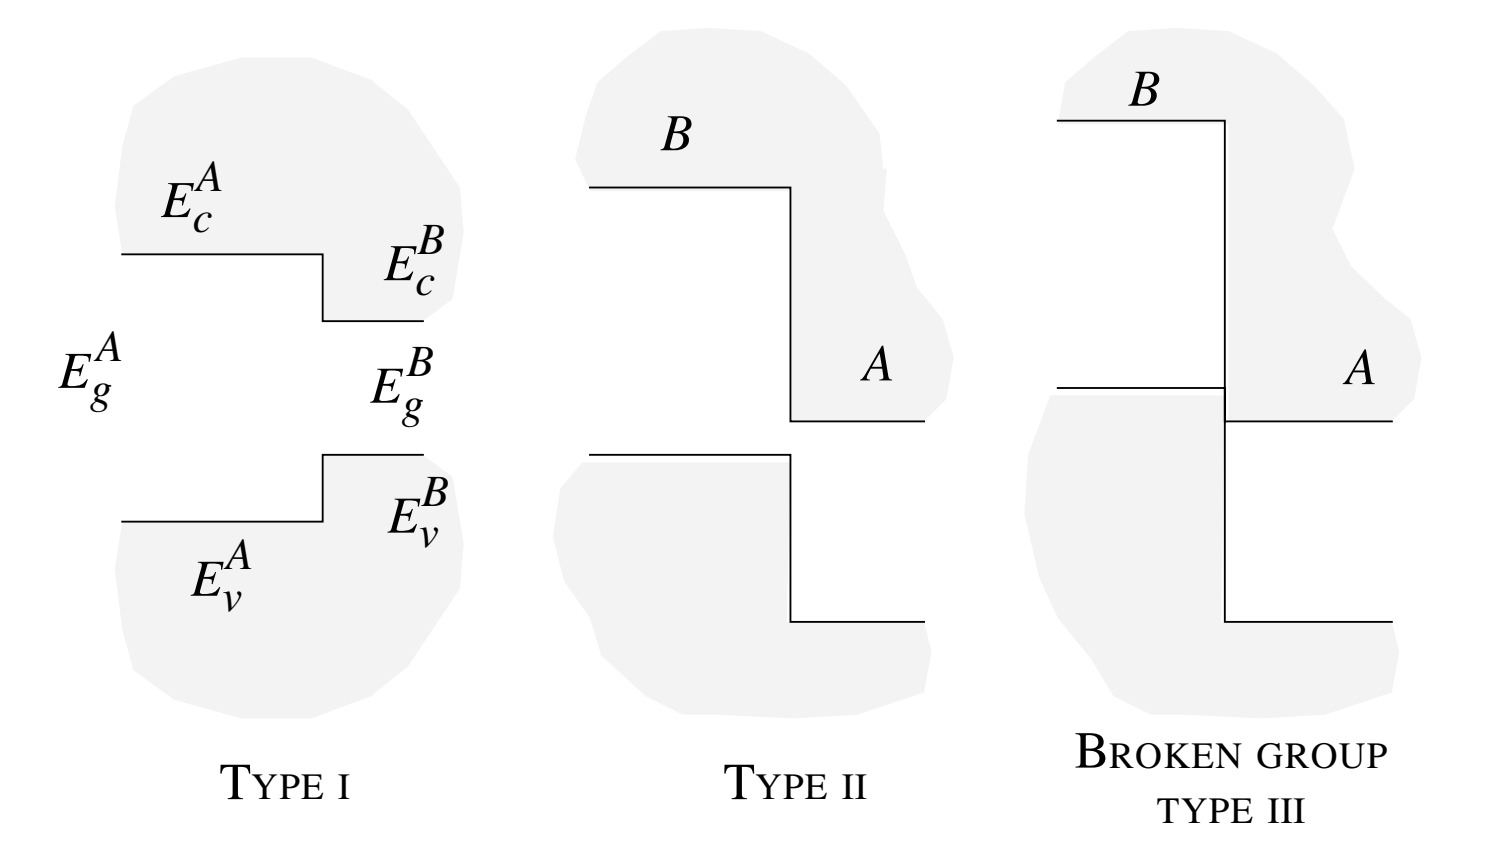
\includegraphics[width=\textwidth]{img/Bandledge_heterostructure.png}
		\\[0.5em]
		\refstepcounter{figure}
		\textbf{Figure~\thefigure.} Various possible bandedge lineups in heterostructure.
		\label{fig:Bandledge_heterostructure}
	\end{minipage}
\end{center}
Once the band alignment is determined, the next step is to describe the electronic states in the heterostructure. A widely used method for this purpose is the \textit{k·p} approach. In its simplest form, the Schrödinger equation for a carrier in a heterostructure can be approximated as:
\begin{equation}
	\left[ -\frac{\hbar^2}{2 m_0} \nabla^2 + V(\mathbf{r}) \right] \psi(\mathbf{r}) = E \psi(\mathbf{r})
	\quad \Rightarrow \quad
	\left[ -\frac{\hbar^2}{2 m^*} \nabla^2 + E_{\text{edge}} \right] \phi = E \phi
\end{equation}
Here, the atomistic potential \( V(\mathbf{r}) \) is replaced by the band-edge energy \( E_{\text{edge}} \), and the complex effect of the crystal environment is incorporated into the effective mass \( m^* \). This simplification forms the basis for the envelope function approximation commonly used in modeling quantum wells and other heterostructures.


\subsection{Bandstructure in Quantum Wells}
To calculate the bandstructure in quantum wells, it is essential to understand the nature of the energy levels and wavefunctions near the edges of the bandgap, as these determine the electronic states in the quantum well. We consider the case where the well region is composed of a direct bandgap semiconductor. In such systems, the conduction band states are primarily of $s$-type character, while the valence band states are $p$-type. Although the formalism can be extended to other material systems, we focus here on a basic quantum well structure.\\
The Schrödinger equation describing the electron states in the quantum well, within the effective mass approximation, is given by:
\begin{equation}
	\left[-\frac{\hbar^2}{2 m^*} \nabla^2 + V(z) \right] \Psi = E \Psi
\end{equation}
Here, \( m^* \) is the effective mass of the electron, and \( V(z) \) is the quantum well potential, which depends only on the growth direction \( z \). The total wavefunction can be separated into its in-plane and out-of-plane components:
\begin{equation}
	\Psi(x, y, z) = e^{i(k_x \cdot x + k_y \cdot y)} f(z)
\end{equation}
\begin{center}
	\begin{minipage}{0.6\textwidth}
		\centering
		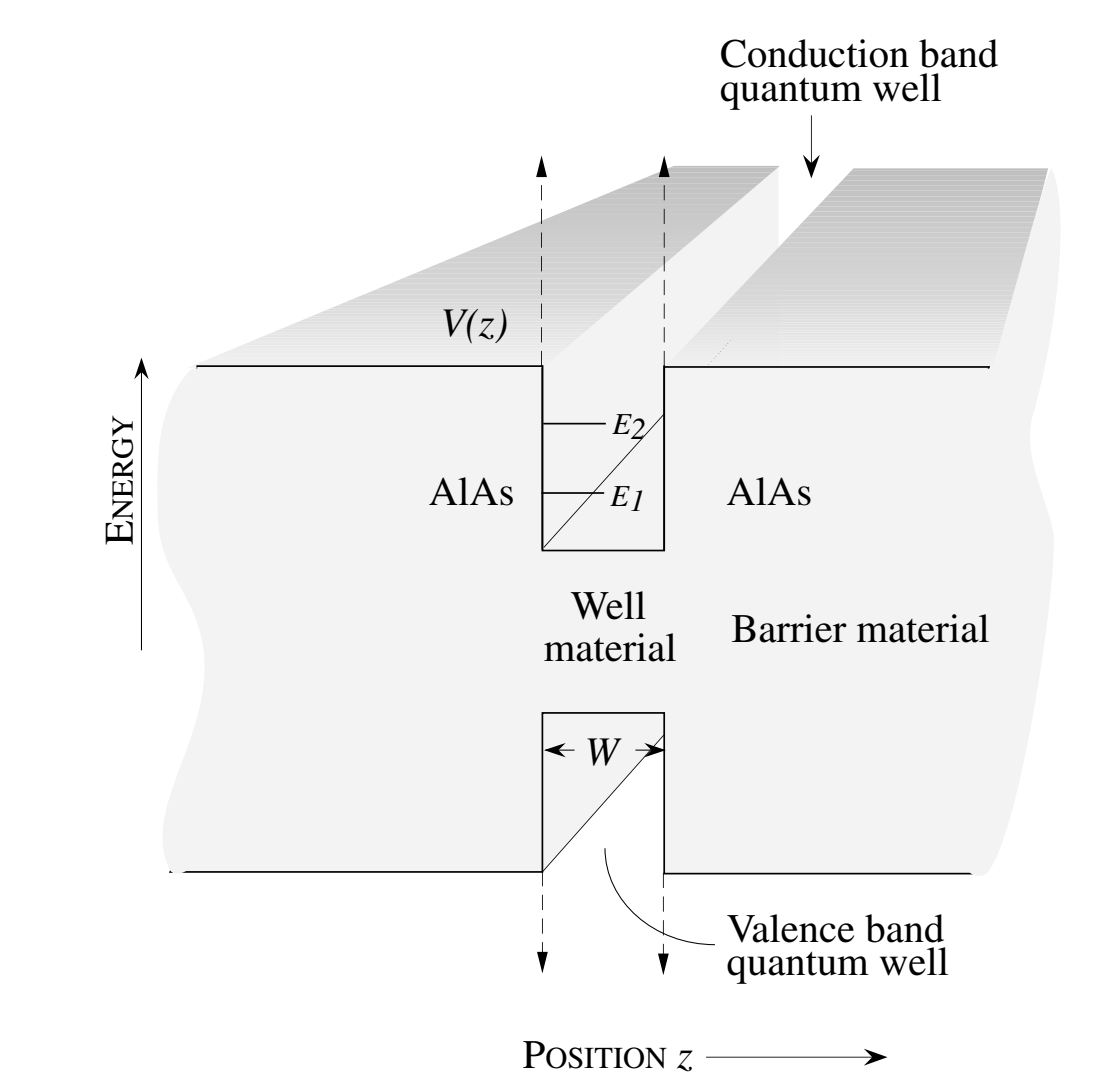
\includegraphics[width=\textwidth]{img/quantum_well_heterostructure.png}
		\\[0.5em]
		\refstepcounter{figure}
		\textbf{Figure~\thefigure.} A quantum well formed for the electron and holes in a heterostructure.
		\label{fig:quantum_well_heterostructure}
	\end{minipage}
\end{center}
Substituting this into the Schrödinger equation yields a one-dimensional equation for \( f(z) \):
\begin{equation}
	\left[-\frac{\hbar^2}{2 m^*} \frac{\partial^2}{\partial z^2} + V(z) \right] f(z) = E_n f(z)
\end{equation}
This one-dimensional quantum well problem is standard and can be found in many undergraduate quantum mechanics texts. Assuming infinite potential barriers, the wavefunctions are:
\[
	f_n(z) =
	\begin{cases}
		\cos\left( \frac{n \pi z}{W} \right), & \text{if } n \text{ is even} \\
		\sin\left( \frac{n \pi z}{W} \right), & \text{if } n \text{ is odd}
	\end{cases}
\]
where \( W \) is the well width. The corresponding quantized energy levels are:
\begin{equation}
	E_n = \frac{\pi^2 \hbar^2 n^2}{2 m^* W^2}
\end{equation}
Including the in-plane kinetic energy contribution, the total energy of the electron becomes:
\begin{equation}
	E(k) = E_n + \frac{\hbar^2 k_\parallel^2}{2 m^*}
\end{equation}
This results in subbands within the conduction and valence bands. If the potential barrier \( V \) is finite, the wavefunction decays exponentially into the barrier region. The solution inside the well remains sinusoidal, but matching boundary conditions leads to the transcendental equations:
\begin{equation}
	\alpha \tan\left( \frac{\alpha W}{2} \right) = \beta \quad \text{or} \quad \alpha \cot\left( \frac{\alpha W}{2} \right) = -\beta
\end{equation}
where
\begin{equation}
	\alpha = \sqrt{\frac{2 m^* E}{\hbar^2}}, \quad \beta = \sqrt{\frac{2 m^* (V_c - E)}{\hbar^2}}
\end{equation}
These equations can be solved numerically to obtain the quantized energy levels \( E_1, E_2, E_3, \dots \), each corresponding to a subband in the quantum well.\\
In the valence band, both heavy hole and light hole subbands exist, and their detailed dispersion relations are affected by strain and confinement. The resulting subband structure plays a significant role in determining the optical and transport behavior of heterostructures.\\
An important consequence of the subband formation is its impact on the density of states (DOS), which influences both optical absorption and carrier dynamics.

For a quantum well, the DOS in the conduction band is:
\begin{equation}
	N(E) = \sum_i \frac{m_i^*}{\pi \hbar^2} \, \sigma(E - E_i)
\end{equation}
where \( \sigma \) is the Heaviside step function and \( E_i \) are the subband energies.

For the valence band, including both heavy and light hole contributions, the DOS becomes:
\begin{equation}
    N(E) = \sum_i \sum_{j=1}^{2} \frac{m_j^*}{\pi \hbar^2} \, \sigma(E_{ij} - E)
\end{equation}
Here, \( j = 1 \) denotes heavy holes and \( j = 2 \) denotes light holes, and \( m_{ij}^* \) are the respective effective masses.\\
In the simplified model described here, the conduction band state is assumed to be purely $s$-type, and a basic effective mass approximation is used. More sophisticated calculations can incorporate full-band models, such as eight-band \textit{k·p} theory, which captures coupling between conduction and valence bands. For unstrained structures, such enhancements do not significantly alter the conduction subband energies. However, for strained heterostructures, a more complete bandstructure model becomes necessary.

\begin{center}
	\begin{minipage}{0.8\textwidth}
		\centering
		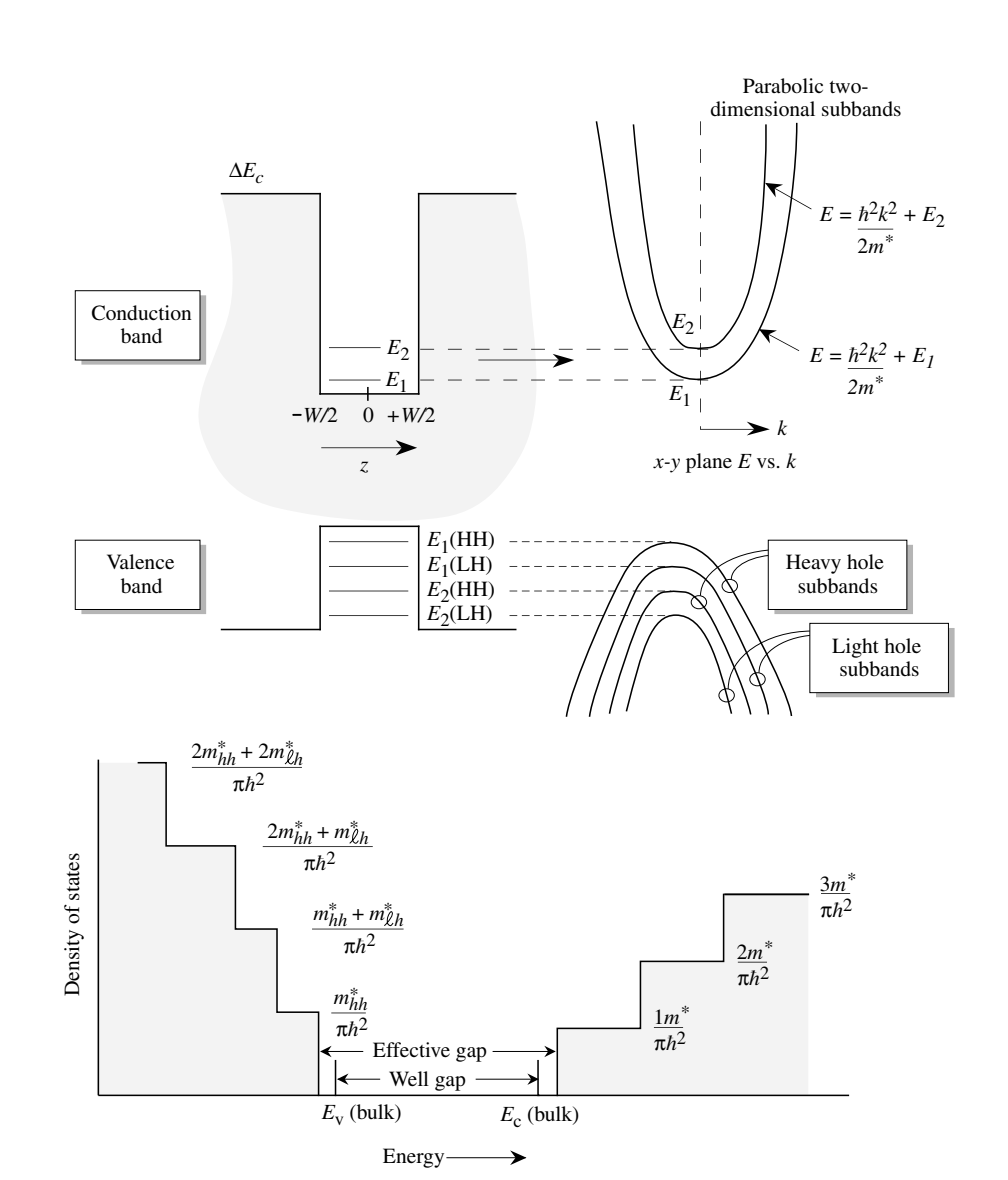
\includegraphics[width=\textwidth]{img/DensityOfState.png}
		\\[0.5em]
		\refstepcounter{figure}
		\textbf{Figure~\thefigure.} Density of states in a 3-, 2-, and 1-dimensional system with a parabolic energy momentum relations.
		\label{fig:DensityOfState}
	\end{minipage}
\end{center}

\subsection{Valence Bandstructure in Quantum Wells}
The description of quantum well bandstructure and density of states outlined earlier is quite accurate for electron states. This is because, in direct bandgap semiconductors, the conduction band is derived predominantly from an $s$-type orbital, and can therefore be treated as a single non-degenerate band. \\
However, the valence band states arise from $p$-type orbitals, leading to the formation of heavy-hole (HH) and light-hole (LH) bands. While the HH states (with total angular momentum $j = 3/2$, $m_j = \pm 3/2$) and LH states ($j = 3/2$, $m_j = \pm 1/2$) are pure and uncoupled at $k = 0$, they exhibit strong mixing as one moves away from the Brillouin zone center.\\
For the purpose of determining subband energy levels, the starting energies can still be calculated separately for HH and LH bands, similarly to the electron case. However, the in-plane ($k_x$–$k_y$) dispersion of hole states is only approximately given by a simple parabolic relation:
\begin{equation}
	E(\mathbf{k}) = E_{n,i} + \frac{\hbar^2 k^2}{2 m_i^*}
\end{equation}
where $i$ denotes either the HH or LH band. A more accurate description of the valence band structure is obtained by solving the Kohn–Luttinger form of the Schrödinger equation:
\begin{equation}
	[H + V_p(z)] \Psi = E \Psi
\end{equation}
Here, $H_p$ is the Kohn–Luttinger Hamiltonian, which in the case of HH and LH coupling becomes a $4 \times 4$ matrix differential operator. Treating the out-of-plane momentum as an operator ($k_z = -i \partial / \partial z$), we obtain the following forms for the Hamiltonian matrix elements:
\begin{equation}
	H_{\text{hh}} = -\frac{\hbar^2}{2m_0} \left[ (\gamma_1 + \gamma_2)(k_x^2 + k_y^2) - (\gamma_1 - 2\gamma_2) \frac{\partial^2}{\partial z^2} \right] + V_p(z)
\end{equation}
\begin{equation}
	H_{\text{lh}} = -\frac{\hbar^2}{2m_0} \left[ (\gamma_1 - \gamma_2)(k_x^2 + k_y^2) - (\gamma_1 + 2\gamma_2) \frac{\partial^2}{\partial z^2} \right] + V_p(z)
\end{equation}
\begin{equation}
	c = \sqrt{3} \frac{\hbar^2}{2 m_0} \left[\gamma_2(k_x^2 - k_y^2)- 2 i \gamma_3 k_x k_y\right]
\end{equation}
\begin{equation}
	b = -i \sqrt{3} \frac{\hbar^2}{m_0} \gamma_3 (- k_y - i k_x) \frac{\partial}{\partial z}
\end{equation}
In these expressions, $V(z)$ represents the quantum well confinement potential, and $\gamma_1$, $\gamma_2$, and $\gamma_3$ are the Luttinger parameters describing the anisotropic hole mass.\\
When biaxial strain is present, additional terms must be included in the Hamiltonian to account for strain-induced modifications in the band structure. These will be introduced in later sections.
The general form of the hole wavefunction can be written as:
\begin{equation}
	\Psi^m_{h}(\mathbf{k}_\parallel,z) = \sum_v g^m_v(z) \, U^v(\mathbf{r}) \, e^{i \mathbf{k}_\parallel \cdot \boldsymbol{\rho}}
\end{equation}
Here, $g^m_v(z)$ are envelope functions that depend on the confinement potential along the growth direction, $U^v(\mathbf{r})$ are the bulk valence band Bloch functions, $m$ is the subband index, and $v$ labels the spinor components associated with the total angular momentum $j = 3/2$ states.\\
This formalism provides a more complete and accurate picture of the valence band substructure in quantum wells, particularly when dealing with hole transport, optical transitions, and strain-induced effects.


\section{Strain and Deformation Potential Theory}
The influence of strain on the electronic and optical properties of semiconductors has been studied extensively over several decades. These investigations have been critical for developing a deeper theoretical understanding of semiconductor bandstructure, particularly by identifying the symmetry properties of energy states involved in optically observed transitions.\\
In addition, strain studies have provided valuable insights into the determination of deformation potentials, which play a fundamental role in describing electronic transport under the influence of lattice scattering. Traditionally, strain was introduced into semiconductors through external mechanical means, often employing sophisticated tools such as diamond anvil cells. These experiments were primarily focused on elucidating the fundamental physics of semiconductors.\\
With the development of strained heteroepitaxy, it has become possible to incorporate strain directly during the epitaxial growth process. Remarkably, built-in strains of a few percent can now be achieved simply by depositing a film onto a substrate with a mismatched lattice constant, as discussed in prior sections.\\
Once the strain tensor is known, the deformation potential theory can be employed to compute the effect of strain on the electronic states throughout the Brillouin zone. The perturbation Hamiltonian due to strain is introduced and analyzed within the framework of first-order perturbation theory. It is generally expressed as:
\begin{equation}
	H_{ij} = \sum_{\alpha\beta} D_{ij}^{\alpha\beta} \, \varepsilon_{\alpha\beta}
\end{equation}
Here, \( D_{ij}^{\alpha\beta} \) are the matrix elements of the deformation potential tensor \( D_{ij} \), and \( \varepsilon_{\alpha\beta} \) are the components of the strain tensor. The deformation potential operator \( D_{ij} \) transforms as a second-rank tensor under the crystal’s symmetry operations.\\
This formalism provides a powerful and practical framework for quantifying the influence of strain on semiconductor electronic structure, and is widely used in the analysis
\begin{center}
	\begin{minipage}{0.7\textwidth}
		\centering
		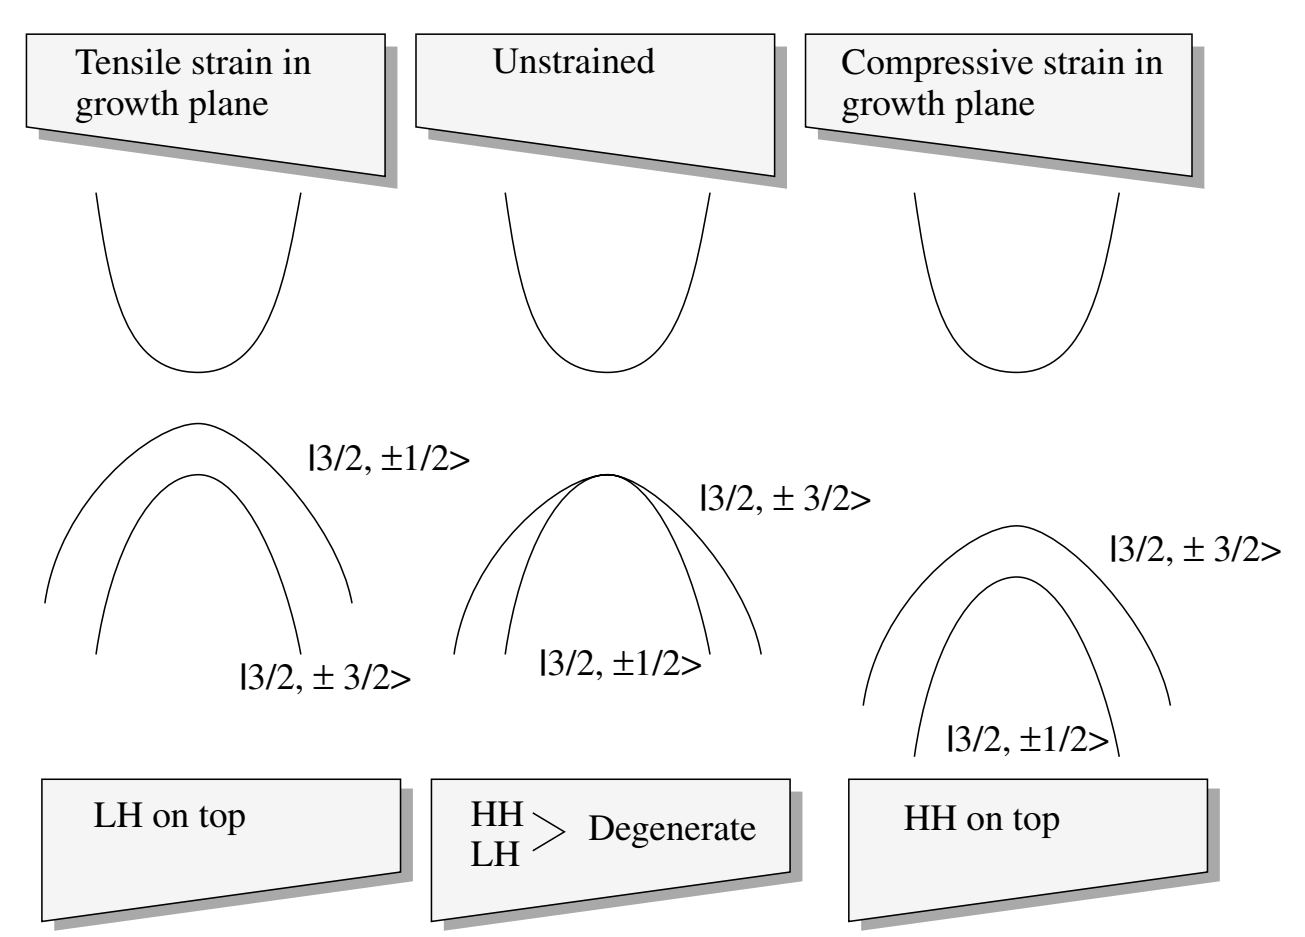
\includegraphics[width=\textwidth]{img/strain_effect.png}
		\\[0.5em]
		\refstepcounter{figure}
		\textbf{Figure~\thefigure.} The effect of strain on the bandstructure of a semiconductor. The conduction band minimum (CBM) and valence band maximum (VBM) shift in response to applied strain. \\
		\label{fig:strain_effect}
	\end{minipage}
\end{center}

Strain introduced in a semiconductor layer grown along the (001) crystallographic direction can significantly modify the band structure, particularly near the band edges. In the case of a direct bandgap semiconductor, the conduction band edge shifts upward or downward relative to its unstrained position, depending on the nature of the strain. However, since the conduction band minimum is typically a non-degenerate state, no splitting occurs under strain.\\
In contrast, the valence band edge is degenerate in the unstrained bulk system. Even in unstrained quantum wells, quantum confinement alone can lift this degeneracy between heavy-hole (HH) and light-hole (LH) states. However, the resulting energy splitting is usually modest, typically on the order of 10–15~meV.\\
When biaxial strain is applied, the impact on the valence band becomes much more pronounced. Under biaxial compressive strain, the bandgap increases and the HH–LH degeneracy is significantly lifted. The energy separation between these states can reach values as large as 100~meV, making strain a powerful tool for engineering the valence band density of states.\\
Specifically, under biaxial compressive strain, the heavy-hole state shifts above the light-hole state. Conversely, under biaxial tensile strain, the light-hole state lies higher in energy than the heavy-hole state. This strain-induced splitting is particularly important for controlling optical transitions and enhancing the performance of optoelectronic devices.
\begin{center}
	\begin{minipage}{0.7\textwidth}
		\centering
		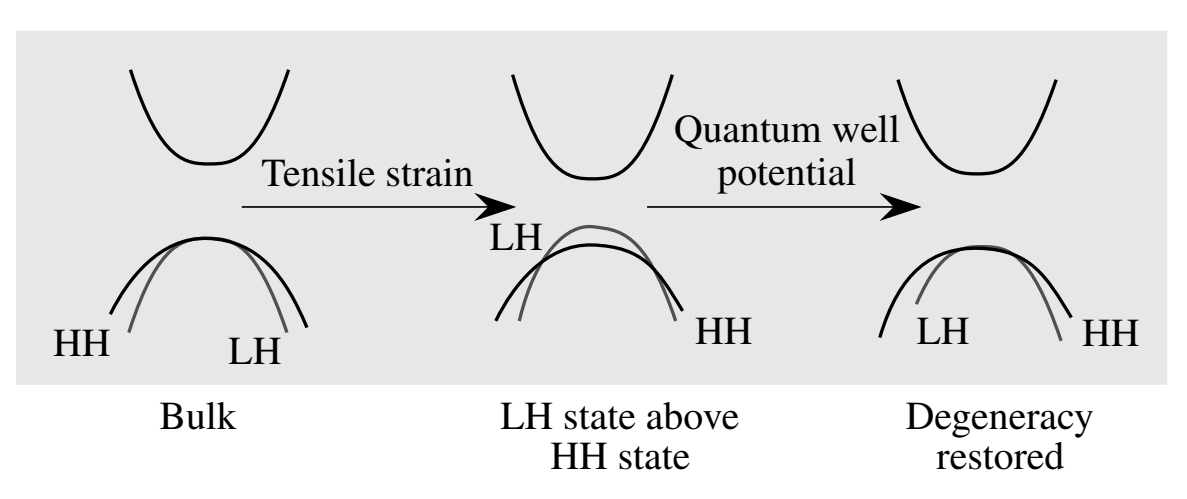
\includegraphics[width=\textwidth]{img/Tensile_Strain.png}
		\\[0.5em]
		\refstepcounter{figure}
		\textbf{Figure~\thefigure.} Effect of biaxial tensile strain and quantum confinement on conduction and valence band states. With appropriate tensile strain, heavy-hole and light-hole states can become degenerate at $\mathbf{k} = 0$ within a quantum well structure.
		\label{fig:tensile_strain}
	\end{minipage}
\end{center}

\subsection{Strained Quantum Wells}
Due to limitations imposed by critical thickness, most strained layers grown by epitaxy are implemented in the form of quantum wells. In these structures, both the effective bandgap and the carrier effective masses are strongly influenced by the presence of strain.\\
As previously discussed, strain—particularly biaxial strain—has a pronounced effect on the valence band edge states. One of the most significant consequences is the reduction of the band-edge density-of-states effective mass. In some cases, the incorporation of strain can lead to a reduction in this mass by nearly a factor of three.
It is evident from the discussion that strain can be a powerful tool for tailoring the electronic bandstructure of semiconductors. The magnitude of strain considered here is readily achievable through strained-layer epitaxy. Importantly, the induced splitting between heavy-hole and light-hole states in the valence band can reach values on the order of 100~meV. Such splitting is accompanied by significant modifications in the band curvature, which directly influence the effective masses and density of states.\\
It is worth noting that achieving similar levels of uniaxial strain through external mechanical means is extremely challenging. The ability to incorporate such strain epitaxially provides a unique and practical avenue for bandstructure engineering.\\
An important question is whether the strain-induced modifications translate into observable changes in physical properties. This topic will be explored in greater depth in later chapters dealing with transport and optical behavior. As will be shown, the effects are indeed substantial and play a key role in the performance of strained semiconductor devices.


\section{Polar Heterostructures}
We have previously discussed that in certain materials, a net polarization can arise due to various mechanisms such as spontaneous polarization, the piezoelectric effect, or ferroelectricity. In face-centered cubic (fcc) semiconductors, spontaneous polarization does not occur; however, strain-induced effects can still lead to a net polarization.\\
One important consequence of polarization differences in semiconductor heterostructures is the emergence of significant built-in electric fields at interfaces. For example, in a polar heterostructure, the interface electric field can be expressed as:
\begin{equation}
	F = \frac{P}{\varepsilon}
\end{equation}
where \( P \) is the net polarization and \( \varepsilon \) is the dielectric constant of the material. This fixed interfacial charge can be harnessed to induce built-in electric fields, generate band bending, and create mobile charge carriers. With proper structural design, this interfacial charge can effectively serve the role of a delta-doping sheet.\\
In zinc blende semiconductors, the piezoelectric effect is the dominant mechanism for polarization. The polarization induced by strain is given in general by:
\begin{equation}
	P_i = \sum_{k,l} e_{ikl} \, \varepsilon_{kl}
\end{equation}
According to Nye (1957), in zinc blende structures only one independent piezoelectric coefficient exists. In the reduced index notation—where \( xx \Rightarrow 1 \), \( yy \Rightarrow 2 \), \( zz \Rightarrow 3 \), \( yz \Rightarrow 4 \), \( zx \Rightarrow 5 \), and \( xy \Rightarrow 6 \)—the only non-zero components of the piezoelectric tensor are:
\begin{equation}
	e_{14} = e_{25} = e_{36}
\end{equation}
This implies that only shear strain contributes to a finite piezoelectric polarization. As previously discussed, in (100) growth the strain tensor is diagonal, and hence, no piezoelectric polarization arises under such epitaxial conditions. However, when growth is performed along directions such as (111), off-diagonal components of the strain tensor become significant. This results in a strong dipole moment across the quantum well, inducing an internal electric field. The corresponding field is given by:
\begin{equation}
	F = \frac{\sqrt{3} e_{14} \, \varepsilon_{xy}}{\varepsilon_s} \quad V/m
\end{equation}
Here, \( e_{14} \) is the piezoelectric coefficient (typically on the order of \( 0.1 \, \text{C/m}^2 \)), \( \varepsilon_{xy} \) is the off-diagonal strain component, and \( \varepsilon_s \) is the dielectric constant. A strain magnitude of approximately 1\% can generate electric fields as high as \( 10^5 \, \text{V/cm} \), highlighting the importance of piezoelectric effects in strained quantum wells.\\
In wurtzite structures (e.g., InN, GaN, AlN), epitaxial growth is typically conducted along the \( c \)-axis, i.e., in the (0001) or \( (\bar{0}001) \) direction. For a sufficiently thick substrate, the in-plane strain components are given by:
\begin{equation}
	\varepsilon_{xx} = \varepsilon_{yy} = \frac{a_3}{a_0} - 1
\end{equation}
where \( a_s \) is the lattice constant of the substrate and \( a_0 \) is that of the unstrained layer. The strain along the growth direction is determined by:
\begin{equation}
	\varepsilon_{zz} = -2 \frac{c_{13}}{c_{33}} \left( \frac{a_s}{a_0} - 1 \right)
\end{equation}
These strains generate a piezoelectric polarization in the strained layer. For wurtzite crystals, the total polarization due to strain is given by:
\begin{equation}
	P_{pz} = e_{33} \varepsilon_{zz} + e_{31} (\varepsilon_{xx} + \varepsilon_{yy})
\end{equation}
where \( e_{33} \) and \( e_{31} \) are piezoelectric constants. The resulting polarization field is directed along the (0001) axis, corresponding to the Ga-face direction in the crystal, following the convention that places Ga atoms on the upper site of each bilayer.\\
The electric field induced by this polarization can be expressed simply as:
\begin{equation}
	F = \frac{P}{\varepsilon_s}
\end{equation}
Typical material constants for InGaN systems include \( c_{13} \approx 109 \, \text{GPa} \) and \( c_{33} \approx 355 \, \text{GPa} \), yielding a ratio \( 2c_{13}/c_{33} \approx 0.6 \). The piezoelectric and spontaneous polarizations play a major role in determining the band alignment and carrier behavior in group-III nitride heterostructures.

\begin{center}
	\begin{minipage}{0.6\textwidth}
		\centering
		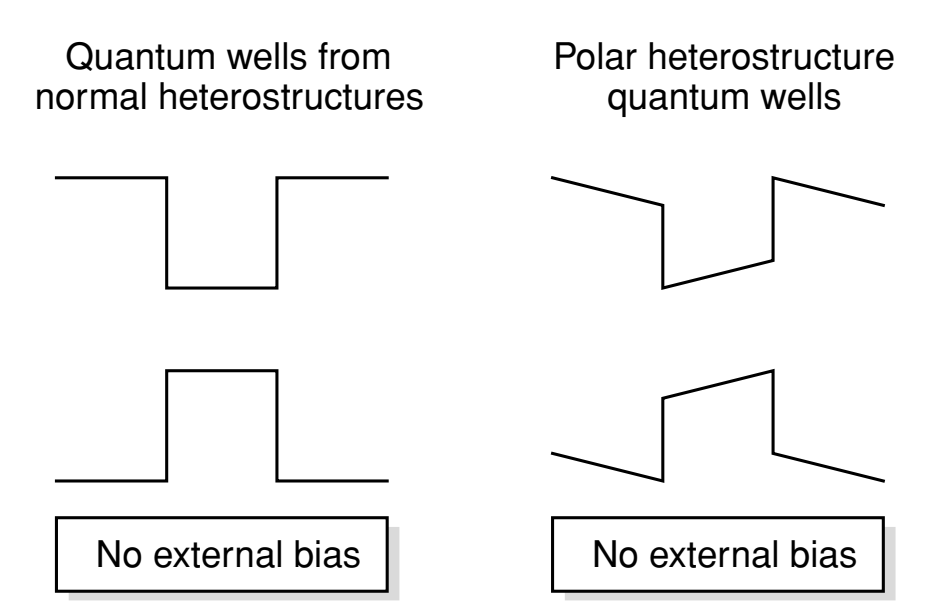
\includegraphics[width=\textwidth]{img/PolarQuantumWell.png}
		\\[0.5em]
		\refstepcounter{figure}
		\textbf{Figure~\thefigure.} A comparison of (undoped) nonpolar and polar quantum well band profiles in the absence of any external electric field.
		\label{fig:polar_quantum_well}
	\end{minipage}
\end{center}
\chapter{Lattice Vibrations and Phonons}

\section{Introduction}
In a crystalline material, atoms are not fixed at rigid lattice sites but vibrate around their equilibrium positions. One of the most important scattering mechanisms for mobile carriers in semiconductors arises from these lattice vibrations. \\
In the earlier discussion on bandstructure, we assumed that the background potential is perfectly periodic and time-independent. However, in real materials, the ions that constitute the crystal lattice are dynamic and undergo thermal vibrations, which become more pronounced with increasing temperature.\\
Scattering results from the disturbances in the periodic potential caused by lattice vibrations. \\
Before addressing how these vibrations lead to scattering, it is essential to first understand the fundamental properties of lattice vibrations themselves. Once these properties are established, we can then analyze how the resulting potential fluctuations contribute to carrier scattering in semiconductors.
\begin{center}
	\begin{minipage}{0.6\textwidth}
		\centering
		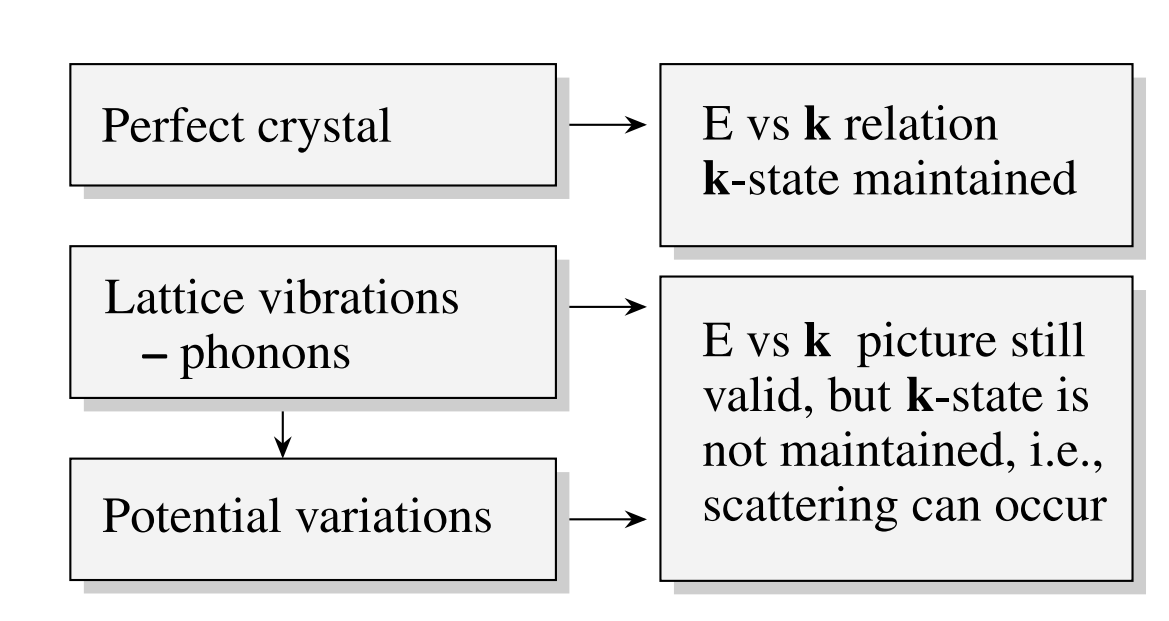
\includegraphics[width=\textwidth]{img/lattice_vibration_effects.png}
		\\[0.5em]
		\refstepcounter{figure}
		\textbf{Figure~\thefigure.}Electron scattering arises from imperfections in the crystal, including lattice vibrations (phonons) and local potential variations, which disrupt coherent transport.
		\label{fig:Lattice_vibration_effects}
	\end{minipage}
\end{center}


\section{Lattice Vibrations}
The reason a particular crystal structure is chosen by a material is fundamentally related to the minimization of the system’s total energy. As atoms approach each other to form a crystal, they experience both attractive and repulsive interactions. The attractive forces can arise from various mechanisms, such as Van der Waals interactions (due to induced dipole moments when electron clouds are perturbed by nearby atoms), ionic bonding (involving electron transfer between atoms), and covalent bonding (where electrons are shared between atoms).\\
When atoms are brought very close, however, there is a strong repulsive interaction primarily due to the Pauli exclusion principle, which prevents electrons on neighboring atoms from occupying the same space.\\
As a result, the total potential energy of the system as a function of interatomic separation exhibits a minimum at some equilibrium spacing \( R_0 \), where the system achieves mechanical stability.

In general, we can expand the crystal binding energy around the equilibrium spacing \( R_0 \) as a Taylor series:
\begin{equation}
	U(R) = U(R_0) + \left.\frac{dU}{dR}\right|_{R_0} \Delta R + \frac{1}{2} \left.\frac{d^2 U}{dR^2}\right|_{R_0} (\Delta R)^2 + \cdots
\end{equation}
\noindent
where \( \Delta R = R - R_0 \) is the deviation from equilibrium.
\begin{center}
	\begin{minipage}{0.6\textwidth}
		\centering
		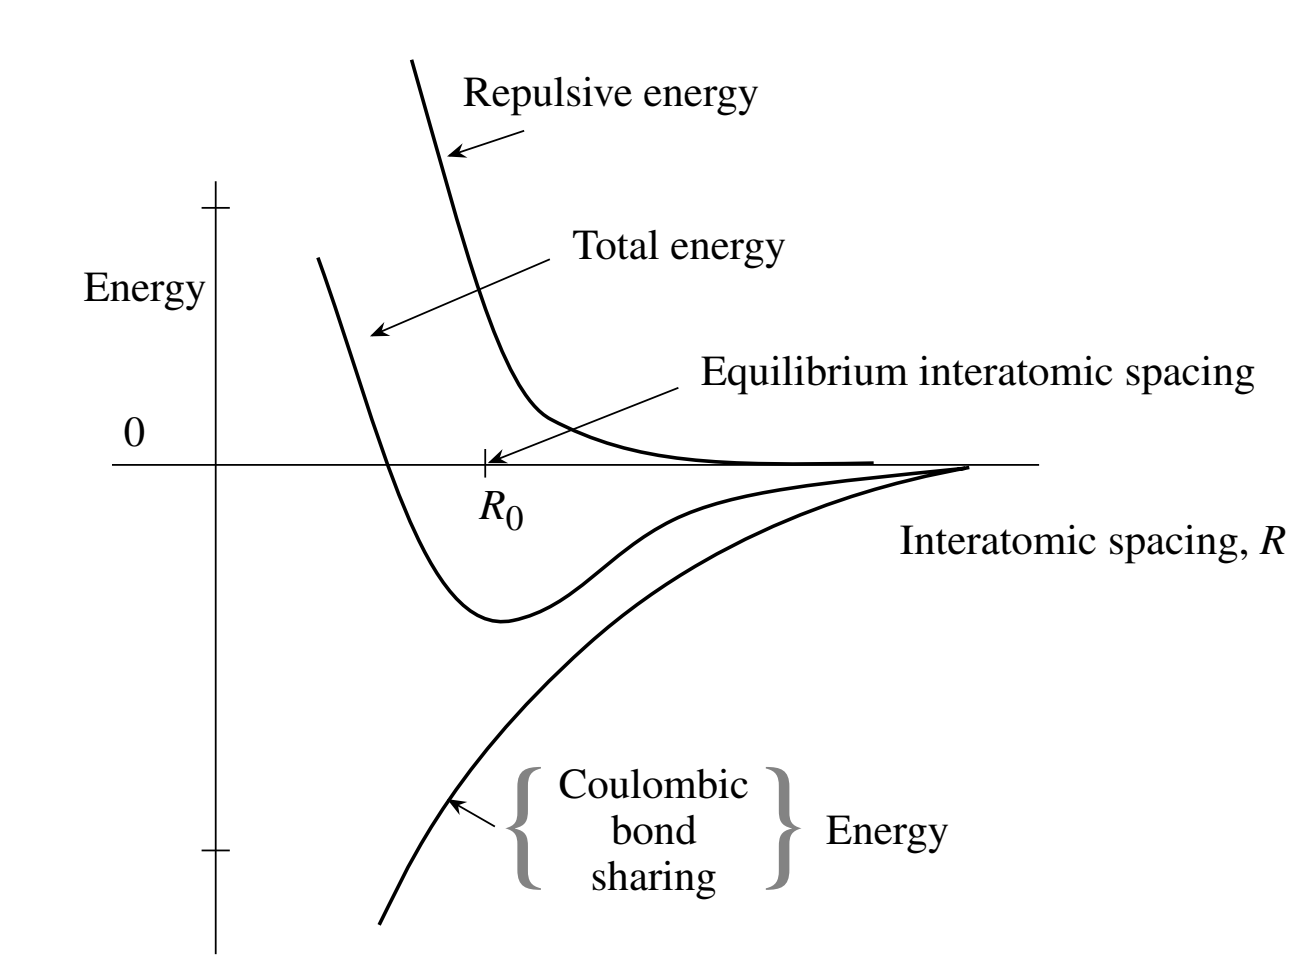
\includegraphics[width=\textwidth]{img/Potential_Energy.png}
		\\[0.5em]
		\refstepcounter{figure}
		\textbf{Figure~\thefigure.}General relationship between binding energy and atomic separation in a crystal. In semiconductors, long-range attraction typically arises from electrostatic interactions or covalent bond energy associated with electron sharing.
		\label{fig:Potential_Energy}
	\end{minipage}
\end{center}
The second term in the expansion is zero since \( R_0 \) is the equilibrium interatomic separation. Retaining terms up to second order in \( \Delta R \), we obtain what is known as the \textit{harmonic approximation}:
\begin{equation}
	U(R) = U(R_0) + \frac{1}{2} C (\Delta R)^2
\end{equation}
where the force constant \( C \) is given by:
\begin{equation}
	C = \left. \frac{\partial^2 U}{\partial R^2} \right|_{R_0}
\end{equation}
The corresponding restoring force is:
\begin{equation}
	F = -C \Delta R
\end{equation}
Due to this restoring force, the atoms in the crystal vibrate similarly to a particle attached to a spring. To analyze such vibrations in semiconductors, consider a diatomic linear lattice (two atoms per basis). The atoms occupy equilibrium positions and vibrate around them. Assuming nearest-neighbor interactions only, and letting \( M_1 \) and \( M_2 \) be the atomic masses, and \( u_s \), \( v_s \) be the displacements of the two atoms in the \( s \)-th unit cell, we write the equations of motion:
\begin{align}
	M_1 \frac{d^2 u_s}{dt^2} & = C (v_s + v_{s-1} - 2u_s) \\
	M_2 \frac{d^2 v_s}{dt^2} & = C (u_s + u_{s+1} - 2v_s)
\end{align}
\begin{center}
	\begin{minipage}{0.8\textwidth}
		\centering
		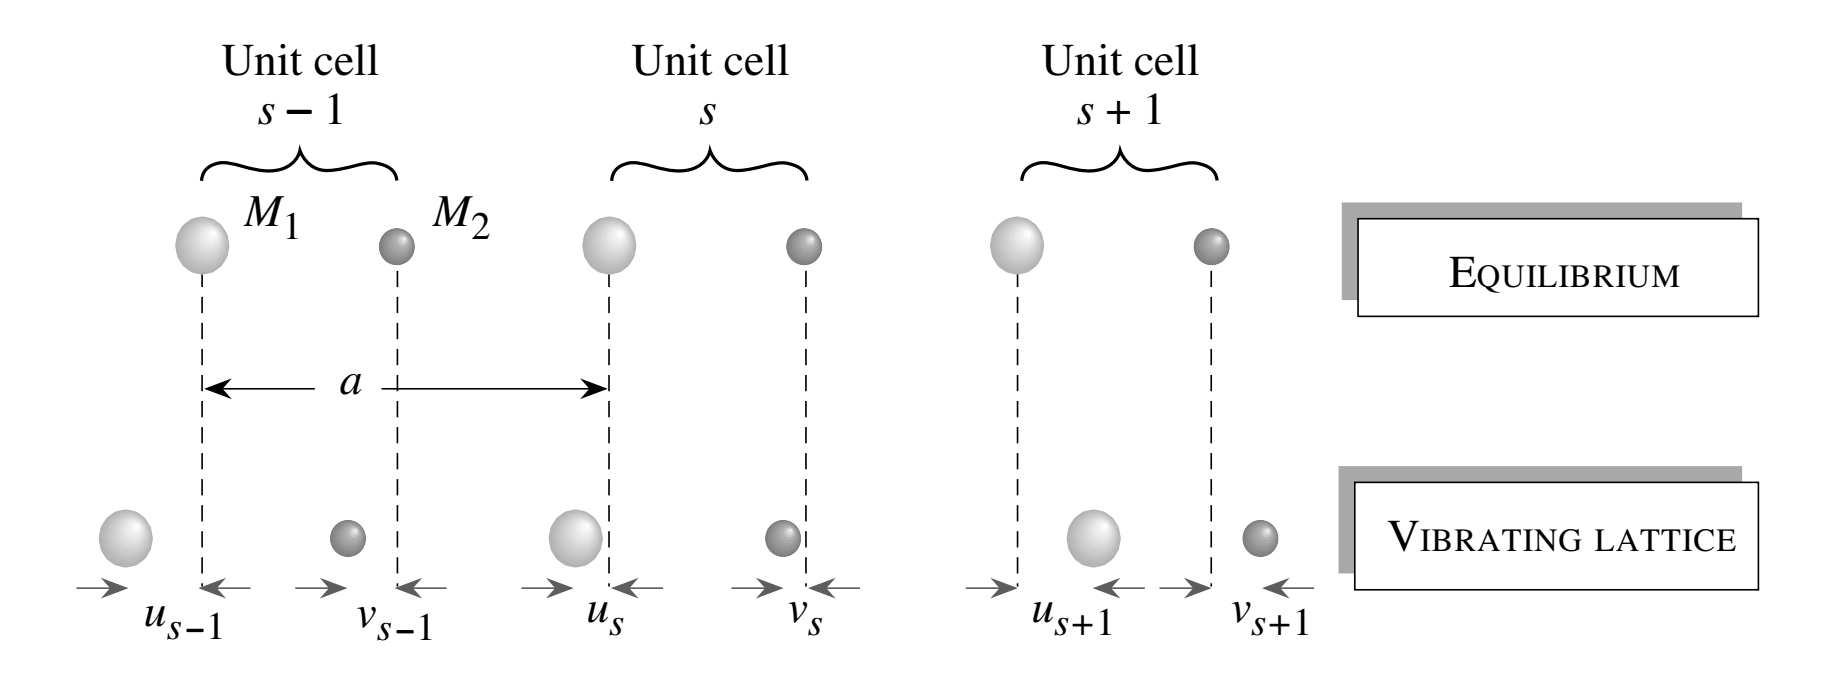
\includegraphics[width=\textwidth]{img/Vibrations.png}
		\\[0.5em]
		\refstepcounter{figure}
		\textbf{Figure~\thefigure.}Lattice vibrations in a crystal with two atoms per unit cell, having masses $M_1$ and $M_2$, connected by a force constant $C$ between adjacent atomic planes.
		\label{fig:Potential_Energy}
	\end{minipage}
\end{center}
We look for traveling wave solutions with alternating amplitudes:
\begin{align}
	u_s & = u \, e^{i s k a} e^{-i \omega t} \\
	v_s & = v \, e^{i s k a} e^{-i \omega t}
\end{align}
Here, \( a \) is the distance between identical planes of atoms (i.e., the lattice periodicity). Substituting into the equations of motion gives:
\begin{align}
	-\omega^2 M_1 u & = C v [1 + e^{-ika}] - 2C u \\
	-\omega^2 M_2 v & = C u [1 + e^{ika}] - 2C v
\end{align}
These form a set of coupled eigenvalue equations, which can be represented in matrix form:
\[
	\begin{pmatrix}
		2C - \omega^2 M_1 & -C(1 + e^{-ika})  \\
		-C(1 + e^{ika})   & 2C - \omega^2 M_2
	\end{pmatrix}
	\begin{pmatrix}
		u \\
		v
	\end{pmatrix}
	= 0
\]
The determinant of this system must vanish:
\[
	\left|
	\begin{matrix}
		2C - \omega^2 M_1 & -C(1 + e^{-ika})  \\
		-C(1 + e^{ika})   & 2C - \omega^2 M_2
	\end{matrix}
	\right| = 0
\]
Expanding and simplifying:
\begin{equation}
	M_1 M_2 \omega^4 - 2C (M_1 + M_2) \omega^2 + 2C^2 (1 - \cos ka) = 0
\end{equation}
Solving this quadratic in \( \omega^2 \), we obtain:
\begin{equation}
	\omega^2 = \frac{2C (M_1 + M_2) \pm \sqrt{4C^2 (M_1 + M_2)^2 - 8C^2 (1 - \cos ka) M_1 M_2}}{2 M_1 M_2}
\end{equation}
Let us consider two limiting cases:
- For small \( k \) (long-wavelength limit), we obtain:
\begin{align}
	\omega_{\text{acoustic}} & \approx \sqrt{\frac{C/2}{M_1 + M_2}} \, ka                                       \\
	\omega_{\text{optical}}  & \approx \sqrt{\frac{2C}{\mu}} \quad \text{with } \mu = \frac{M_1 M_2}{M_1 + M_2}
\end{align}
- At the Brillouin zone boundary \( k = \pi/a \), the frequencies are:
\begin{align}
	\omega_1 & = \sqrt{\frac{2C}{M_1}} \\
	\omega_2 & = \sqrt{\frac{2C}{M_2}}
\end{align}
This analysis yields two distinct branches of lattice vibrations:
\begin{itemize}
	\item The \textit{acoustic branch}, where \( \omega \to 0 \) as \( k \to 0 \), representing sound wave propagation.
	\item The \textit{optical branch}, where \( \omega \) remains finite as \( k \to 0 \), corresponding to out-of-phase motion of the two atoms.
\end{itemize}
The acoustic mode has a linear dispersion relation near \( k = 0 \), and the group velocity (sound speed) is given by:
\begin{equation}
	v_s = \left. \frac{d\omega}{dk} \right|_{k \to 0} = a \sqrt{\frac{C}{M}}, \quad \text{with } M = \frac{M_1 + M_2}{2}
\end{equation}
It is important to examine the eigenfunctions (i.e., the displacement amplitudes \( u_s \)) corresponding to the optical and acoustic branches of the dispersion relation.
For \( k = 0 \), in the case of the \textit{optical branch}, the angular frequency is given by:
\begin{equation}
	\omega^2 = 2C \left( \frac{1}{M_1} + \frac{1}{M_2} \right)
\end{equation}
\begin{center}
	\begin{minipage}{0.8\textwidth}
		\centering
		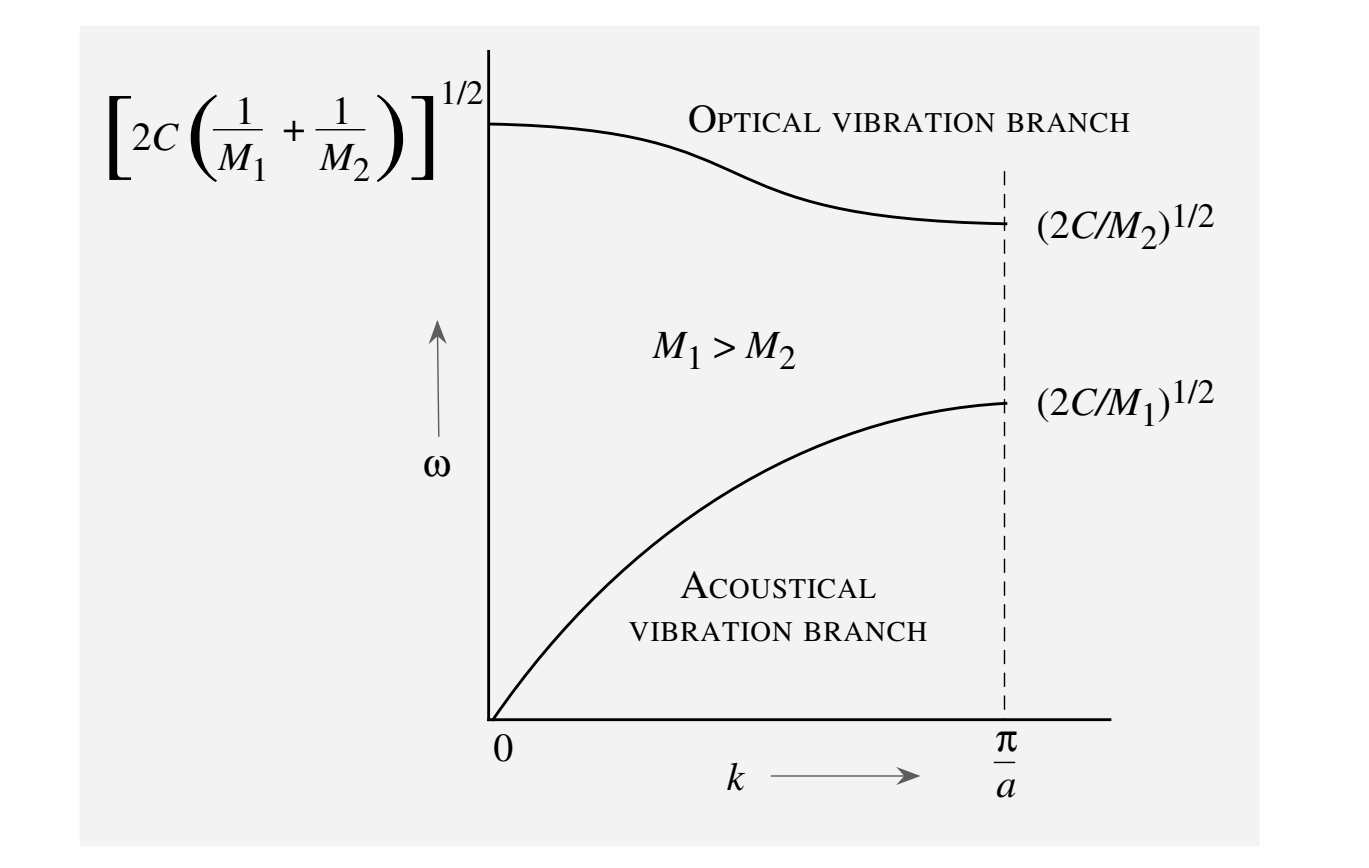
\includegraphics[width=\textwidth]{img/OpticalVSAcoustic_differences.png}
		\\[0.5em]
		\refstepcounter{figure}
		\textbf{Figure~\thefigure.}
		\label{fig:OpticalVSAcoustic_differences}
	\end{minipage}
\end{center}
Substituting this value into the equation of motion, we obtain the relation between the amplitudes of the atomic displacements:
\begin{equation}
	u = -\frac{ M_2}{M_1} v
\end{equation}
In this case, the two atoms vibrate against each other, such that their center of mass remains stationary. This describes an out-of-phase motion, which is characteristic of optical phonons.
In contrast, for the \textit{acoustic branch}, in the long-wavelength limit (\( k \to 0 \)), the solution leads to:
\begin{equation}
	u = v
\end{equation}
This corresponds to both atoms moving in phase, i.e., the entire lattice unit oscillates as a whole, which is characteristic of sound wave propagation.
Furthermore, for each wavevector \( k \), there exist three possible vibrational modes:
\begin{itemize}
	\item One \textbf{longitudinal mode}, where atomic displacements are parallel to the direction of wave propagation.
	\item Two \textbf{transverse modes}, where atomic displacements are perpendicular to the direction of wave propagation.
\end{itemize}
In general, these modes have different frequencies because the restoring forces differ for longitudinal and transverse motions.\\
In ionic crystals such as GaAs, the \textit{optical vibrations} induce oscillating dipole moments due to the displacement of positive and negative ions relative to each other. These polarization fields interact with the vibrations, especially in the longitudinal mode. This interaction introduces an additional long-range restoring force for the longitudinal optical (LO) phonons, increasing their frequency relative to the transverse optical (TO) phonons.\\
As a result, in such materials, the LO phonon frequency is greater than the TO phonon frequency at the zone center (\( k = 0 \)). This splitting is a fundamental feature of polar optical phonons in ionic semiconductors.
\begin{center}
	\begin{minipage}{0.9\textwidth}
		\centering
		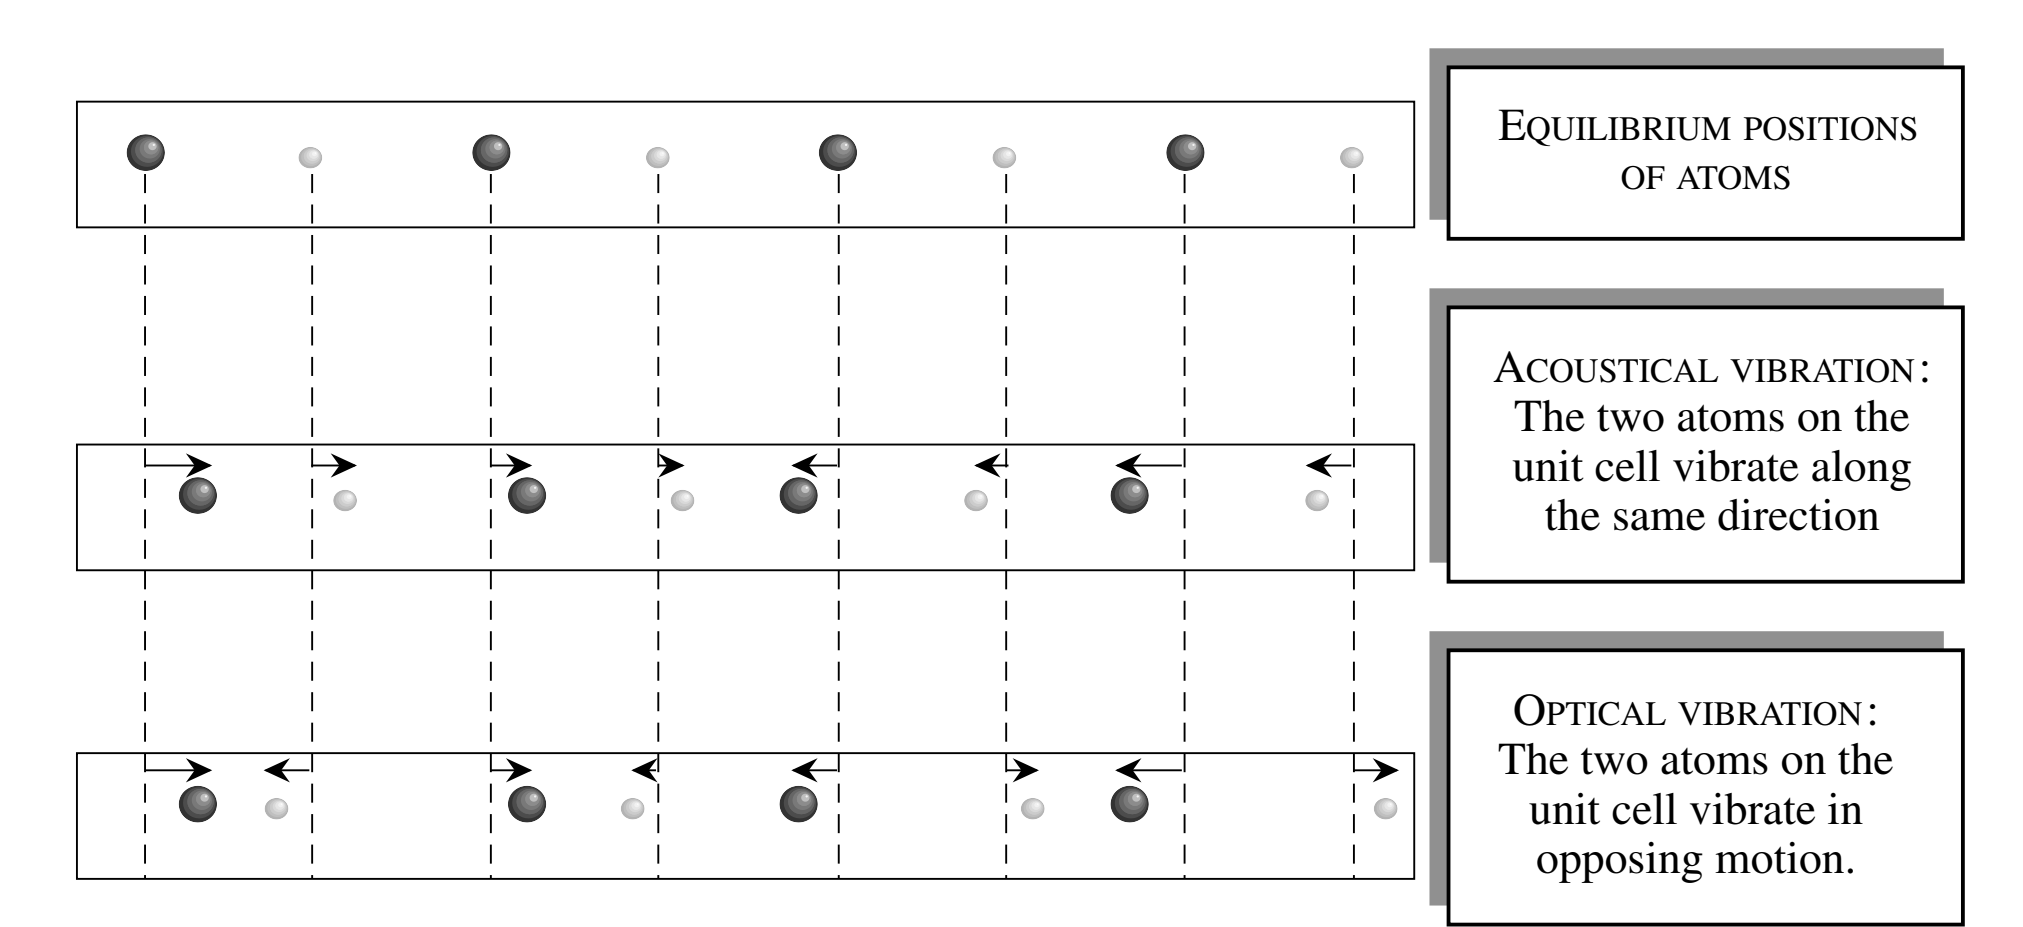
\includegraphics[width=\textwidth]{img/acoustic&opticalmode.png}
		\\[0.5em]
		\refstepcounter{figure}
		\textbf{Figure~\thefigure.}Difference between as acoustical mode an optical mode.
		\label{fig:OpticalVSAcoustic_differences}
	\end{minipage}
\end{center}

\subsection{Phonon: Quantization of Lattice Vibrations}
In the previous discussions, we evaluated the dispersion relation \( \omega \) vs. \( k \) for a set of coupled harmonic oscillator equations. If we now consider a single harmonic oscillator problem in quantum mechanics with the Hamiltonian:
\begin{equation}
	H = \frac{P^2}{2m} + \frac{1}{2} C x^2
\end{equation}
\noindent
the energy of the vibrating particle is quantized and given by:
\begin{equation}
	\epsilon_n = \left(n + \frac{1}{2}\right)\hbar\omega, \quad n = 0, 1, 2, \dots
\end{equation}
\noindent
where \( \omega = \sqrt{C/m} \) is the classical frequency of oscillation.
In classical physics, the oscillator energy can vary continuously with the amplitude of vibration. However, in quantum mechanics, the oscillator has a minimum energy of \( \hbar \omega / 2 \) and its energy increases in discrete steps of \( \hbar \omega \).
In the framework of second quantization, the integer \( n \) represents the number of "particles" or quanta of vibrational energy in the system. These quanta are called \textit{phonons}. A phonon is the quantized mode of lattice vibration, analogous to how a photon is the quantum of light.\\
For a single oscillator, the frequency \( \omega \) is fixed. However, in a crystal made up of many coupled atoms (i.e., coupled oscillators), the vibrational frequencies span a range. These are indexed by a wavevector \( k \), leading to a dispersion relation \( \omega(k) \). The quantized energy for a given wavevector \( k \) is:
\begin{equation}
	\epsilon_k = \left(n_\mathbf{k} + \frac{1}{2}\right) \hbar \omega_\mathbf{k}
\end{equation}
\noindent
where \( n_\mathbf{k} \) is the number of phonons in the mode with wavevector \( \mathbf{k} \) and frequency \( \omega_\mathbf{k} \).\\
To determine how many phonons occupy a given mode, we will later define the appropriate statistical distribution for phonons.
The allowed wavevectors \( k \) in a crystal with \( N \) unit cells and periodic boundary conditions are given by:
\begin{equation}
	|\mathbf{k}| = \frac{2\pi n}{Na}, \quad n = 0, \pm 1, \dots, \pm \left(\frac{N}{2} - 1\right)
\end{equation}
\noindent
This quantization implies there are a total of \( 3N \) vibrational modes in the crystal: \( N \) longitudinal and \( 2N \) transverse modes. Each mode can have an integer occupation number \( n_k \) determined by phonon statistics.


\section{Phonon Statistics}
We have briefly introduced the concept that lattice vibrations can be quantized in terms of particles known as $k$-phonons. To determine how many phonons occupy a specific vibrational mode with angular frequency $\omega$ at a given temperature $T$, one must consider the relevant statistical distribution. Phonons, being bosonic in nature, are governed by Bose–Einstein statistics under conditions of thermal equilibrium.\\
The average phonon number in a mode with frequency $\omega$ is expressed as:
\begin{equation}
	\langle n_{\omega} \rangle = \frac{1}{\exp\left( \frac{\hbar \omega}{k_B T} \right) - 1}
\end{equation}
\begin{center}
	\begin{minipage}{0.5\textwidth}
		\centering
		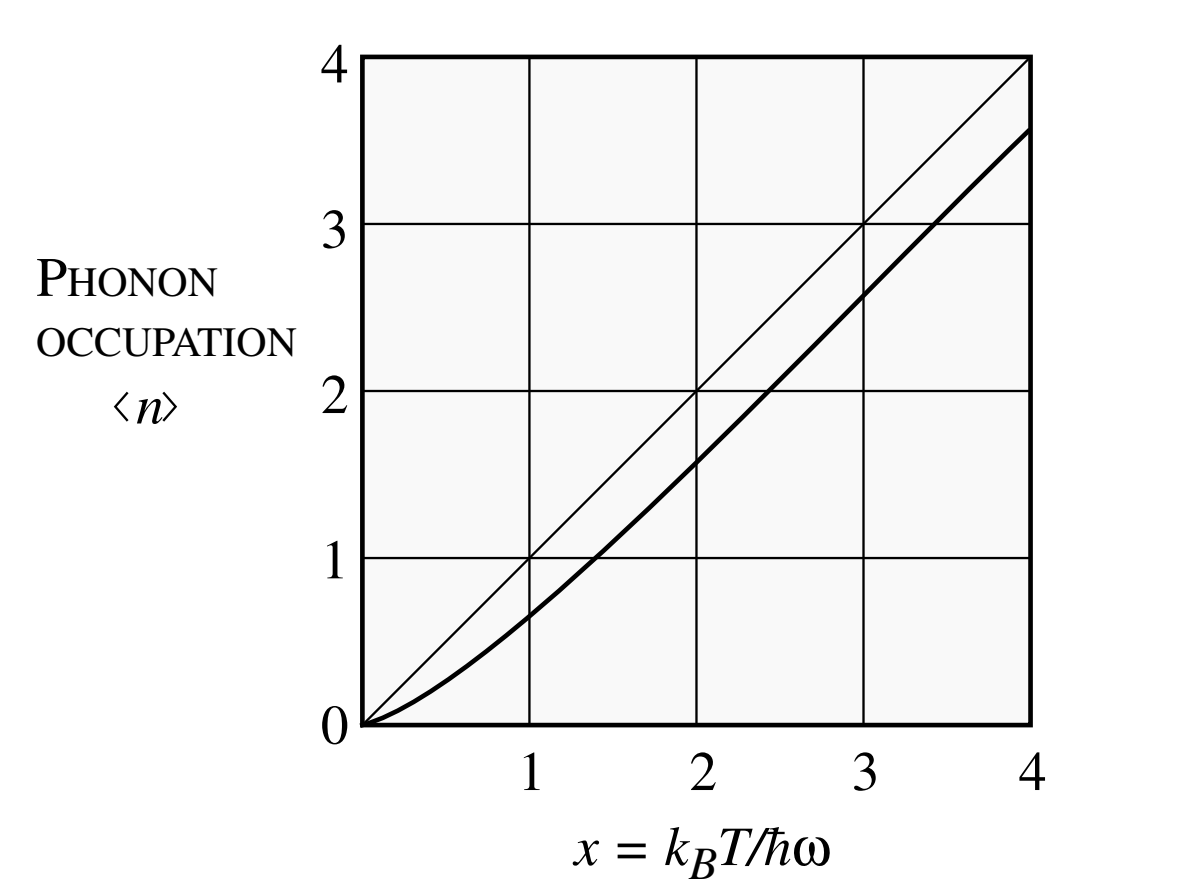
\includegraphics[width=\textwidth]{img/BoseEinstein_distribution.png}
		\\[0.5em]
		\refstepcounter{figure}
		\textbf{Figure~\thefigure.} Bose-Einstein distribution.
		\label{fig:BoseEinstein_distribution}
	\end{minipage}
\end{center}
Unlike electrons, whose occupancy follows the Fermi–Dirac distribution and is restricted to at most one particle per state, bosons such as phonons are permitted to share quantum states. Consequently, the occupation number for phonons can exceed unity. As temperature increases, lattice vibrations become more intense, leading to a higher average phonon population, $\langle n_{\omega} \rangle$.\\
It is worth highlighting that at lower temperatures, the occupation of optical phonons remains minimal due to their relatively high energy at any wavevector $k$. In contrast, acoustic phonons, which can have very small $\hbar \omega$ values at low $k$, maintain significant occupancy even at low temperatures. Therefore, optical phonons contribute less significantly at low temperatures.\\
In the limiting case where $\hbar \omega \ll k_B T$, the phonon occupation number simplifies to:
\begin{equation}
	\langle n \rangle \approx \frac{k_B T}{\hbar \omega}
\end{equation}
The total energy associated with the lattice vibrations, neglecting the zero-point energy, is given by summing over all wavevectors $k$ and polarizations $\rho$:
\begin{equation}
	U = \sum_{\mathbf{k}, \rho} \langle n_{\mathbf{k}, \rho} \rangle \hbar \omega_{\mathbf{k}, \rho}
\end{equation}
Here, $\mathbf{k}$ represents the phonon wavevector and $\rho$ denotes the polarization index of each vibrational mode.

\subsection{Conservation Laws in Scattering of Particles involving Phonons}
A phonon characterized by a wave vector $\mathbf{k}$ can interact with other particles such as electrons or photons, imparting momentum as though it carries a value $\hbar \mathbf{k}$. It is important to recall that for electrons, the quantity $\hbar \mathbf{k}$ (related to the wave vector) represents the relevant momentum, rather than the actual mechanical momentum of the particle. Although phonons are treated as if they possess momentum, they do not carry any real physical momentum. This is because lattice vibrations involve atoms oscillating about their equilibrium positions in opposite directions, meaning the overall motion of the crystal remains unchanged. Thus, the net physical momentum associated with lattice vibrations is zero.\\
This can also be demonstrated mathematically. The total momentum of the crystal can be expressed as:
\begin{equation}
	\mathbf{p} = M \frac{d}{dt} \sum_s \mathbf{u}_s
\end{equation}
where $M$ is the total mass and $\mathbf{u}_s$ denotes the displacement of atom $s$. Given the form of the vibrational solution, this summation evaluates to zero, which aligns with the physical expectation that the center of mass of the crystal does not move.\\
When examining electron-phonon interactions, it is found that first-order phonon scattering processes must obey conservation laws. Specifically, the conservation of crystal momentum and energy leads to the following relations:
\begin{equation}
	\mathbf{k}_i = \mathbf{k}_f \pm \mathbf{q}
\end{equation}
\begin{equation}
	\mathbf{E}_i = \mathbf{E}_f \pm \hbar \omega_{\mathbf{q}}
\end{equation}
Here, $\mathbf{k}_i$ and $\mathbf{k}_f$ represent the initial and final wave vectors of the electron, $\mathbf{q}$ is the phonon wave vector, and $\mathbf{E}_i$, $\mathbf{E}_f$, and $\hbar \omega_{\mathbf{q}}$ correspond to the respective energies involved. For more intricate scattering events involving multiple phonons, these conservation laws are extended accordingly to account for the additional complexity.

\section{Polar Optical Phonons}
In previous discussions concerning optical phonons, we have not accounted for the fact that, in certain semiconductors, the constituent atoms possess net charges—specifically, positive and negative ions such as cations and anions. This ionic characteristic is not present in group IV elemental semiconductors like Si, Ge, or C. However, in compound semiconductors, the ionic nature gives rise to an additional restoring force due to long-range polarization fields that accompany lattice vibrations.
\begin{center}
	\begin{minipage}{0.8\textwidth}
		\centering
		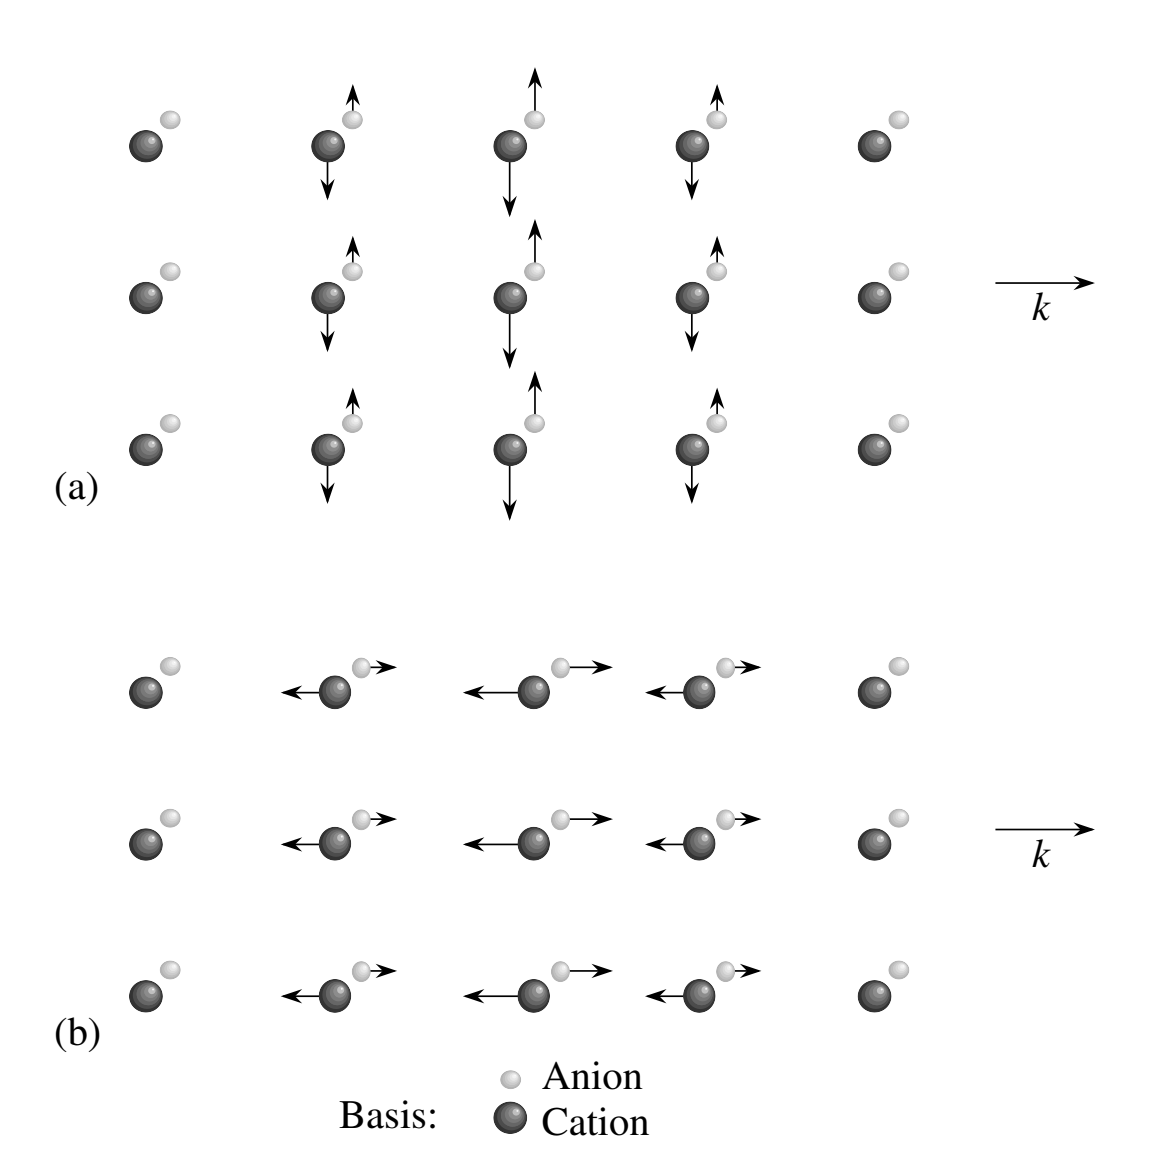
\includegraphics[width=\textwidth]{img/OpticalModes.png}
		\\[0.5em]
		\refstepcounter{figure}
		\textbf{Figure~\thefigure.} Optical vibrations in an ionic crystal.(a) Transverse optical modes do not induce macroscopic polarization. (b) Longitudinal optical modes generate long-range electric fields due to polarization effects.

		\label{fig:OpticalModes}
	\end{minipage}
\end{center}
To examine this phenomenon, we consider two conceptual approaches. The first, although highly simplified, effectively illustrates the essential physical concepts. We work in terms of the relative displacement vector
\begin{equation}
	\mathbf{u}_r = \mathbf{u} - \mathbf{v}
\end{equation}
which denotes the relative motion between the sublattices of positively and negatively charged ions. For transverse vibrational modes, which do not generate macroscopic polarization, the equation of motion takes the form
\begin{equation}
	M \ddot{\mathbf{u}}_r + M \omega_t^2 \mathbf{u}_r = 0
\end{equation}
where $M$ is the reduced mass of the two atoms, and $\omega_t$ is the transverse optical phonon frequency.\\
In contrast, longitudinal vibrational modes induce an electric field as a result of polarization. The equation of motion in this case incorporates both the mechanical restoring force and the force due to the induced electric field, yielding
\begin{equation}
	- \omega_l^2 M \mathbf{u}_r = - \omega_t^2 M \mathbf{u}_r + \mathbf{F}_i e^*
\end{equation}
Here, $\mathbf{F}$ represents the internal electric field generated by polarization, and $e^*$ is an effective charge per ion. Assuming $n$ unit cells per unit volume, the polarization is given by
\begin{equation}
	\mathbf{P} = n e^* \mathbf{u}_r
\end{equation}
The associated electric field in a vacuum, using $\varepsilon_0$ as the permittivity of free space, is
\begin{equation}
	\mathbf{F} = -\frac{\mathbf{P}}{\varepsilon_0} = -\frac{n e^* \mathbf{u}_r}{\varepsilon_0}
\end{equation}
Substituting this into the equation of motion leads to a corrected expression for the longitudinal optical phonon frequency:
\begin{equation}
	\omega_l^2 = \omega_t^2 + \frac{n {e^*}^2}{\varepsilon_0 M}
\end{equation}
If the material possesses a static relative dielectric constant $\varepsilon_r$ such that $\varepsilon = \varepsilon_r \varepsilon_0$, the equation becomes
\begin{equation}
	\omega_l^2 = \omega_t^2 + \frac{n \epsilon_{rel} {e^*}^2}{M \varepsilon_0}
\end{equation}
The effective charge $e^*$ will be addressed further in the context of polar optical phonon scattering. It should be noted that the longitudinal optical phonon frequency exceeds that of the transverse phonons near the Brillouin zone center ($k \approx 0$). In group IV elemental semiconductors, no such frequency splitting exists at $k = 0$ due to the absence of ionicity. However, in III–V compound semiconductors, the difference becomes significant because of their polar nature.\\
An important observation is that optical phonons exhibit minimal dispersion near $k = 0$; their energy bands are nearly flat, unlike those of acoustic phonons. Accordingly, in future discussions on electron-phonon scattering, we will assume that optical phonons are dispersionless.

\section{Phonons in Heterostructures}
It is evident that the behavior of phonons bears a strong resemblance to that of electrons, as both phenomena involve solving differential equations within a periodic potential. In the context of heterostructures, the concept of electronic band structure has already been explored, particularly in relation to systems such as quantum wells and superlattices. These same structural configurations exert a notable influence on phonon dispersion, much like their effect on electronic spectra.\\
The distinction between the electronic and phononic cases, however, lies primarily in the characteristic length scales involved. For electrons, the band offsets in semiconductors give rise to heterostructure effects when the quantum well dimensions approach the electron de Broglie wavelength, typically on the order of 100~\AA. In contrast, for phonons, the relevant length scales are considerably shorter—on the order of a few monolayers.\\
Consequently, there exist phonon modes that are uniquely associated with interfaces and with superlattices of narrow periodicity. These interface-related phonon modes can play a significant role in determining the thermal and vibrational properties of the heterostructure.
\subsection{Confined Optical Phonons}
In superlattices with narrow periodicity, phonon modes can become confined within individual layers, in much the same way that electron wavefunctions are confined within a quantum well. A notable example of this occurs in systems composed of alternating layers of GaAs and AlAs. The optical phonon dispersion relations of these two materials do not intersect, implying that optical modes originating in one material are unable to propagate into the adjacent layer. As a result, these phonon modes are spatially confined to their respective layers.

This confinement leads to a situation analogous to a particle in an infinite square potential well. The permitted wave vectors for such confined modes are quantized according to the relation
\begin{equation}
	|k_n| = \frac{n}{2d}, \quad \text{for } n = 1, 2, 3, \dots
\end{equation}
where $d$ denotes the thickness of the individual GaAs or AlAs layer. Remarkably, the energies of these confined phonon modes have been observed to closely follow the dispersion curves of the corresponding bulk materials. That is, the function $E(k)$ remains nearly unchanged whether evaluated at the continuous $k$ values characteristic of bulk GaAs or at the discrete $k$ values dictated by quantization within the confined layer.
\subsection{Interface Phonons}
In semiconductor heterostructures, there also exist vibrational modes within the optical phonon frequency range that are characterized by having their maximum amplitude localized at the interfaces between two distinct materials. These so-called interface modes are of particular interest because they are accompanied by macroscopic electric fields.
Such modes can be effectively understood using a simplified electrostatic model. The discontinuity in material properties across the interface—such as dielectric constants and ionic character—gives rise to polarization effects, which in turn generate electric fields associated with the vibrational modes.\\

\section{Phonon Scattering: General Formalism}
In our treatment of electronic bandstructure, we have assumed a static, time-independent periodic potential as the background. This assumption enables the derivation of electronic bands. In contrast, lattice vibrations introduce a time-dependent aspect to the crystal potential, leading to the quantized vibrational excitations known as phonons and their associated dispersion relations.\\
The possibility of separating, at first order, the electronic behavior from lattice dynamics relies on the validity of the adiabatic approximation. This approximation is applicable to systems where the time dependence of the Hamiltonian evolves slowly enough that, at each instant, the system can be regarded as effectively time-independent. While phonon frequencies fall in the terahertz range—on the order of $10^{12}$ Hz—this still qualifies as “slow” compared to electronic time scales due to the large difference in mass between electrons and nuclei. As such, the adiabatic approximation proves to be highly effective, allowing us to proceed in two distinct stages:
\begin{enumerate}
	\item Determine the electronic states in a perfect lattice, yielding the electronic bandstructure.
	\item Analyze the interactions between electrons and lattice vibrations, or phonon scattering.
\end{enumerate}
In previous sections, it has been shown that in semiconductors with two atoms per basis, both acoustic and optical phonon modes arise. Near the Brillouin zone center ($k = 0$), acoustic phonons exhibit a linear relationship between $\omega$ and $k$, while optical phonons are nearly dispersionless. Each of these types of phonons exists in both longitudinal and transverse polarization modes. The motion of atoms within the lattice produces strain, which, according to deformation potential theory, leads to perturbations in the electronic energy levels. This relationship has already been explored in the context of strain-induced modifications to bandstructure.\\
Generally, the interaction between electrons and phonons depends on the atomic displacement $\mathbf{u}$. The resulting perturbation potential $U$ takes different forms depending on the type of phonon:
\begin{align*}
	\text{Acoustic phonons:} \quad            & U \sim D \frac{\partial u}{\partial x} \\
	\text{Optical phonons (non-polar):} \quad & U \sim D_0 u                           \\
	\text{Polar optical phonons:} \quad       & U \sim e^* u
\end{align*}
Here, $e^*$ is an effective charge per ion.\\
\begin{center}
	\begin{minipage}{0.5\textwidth}
		\centering
		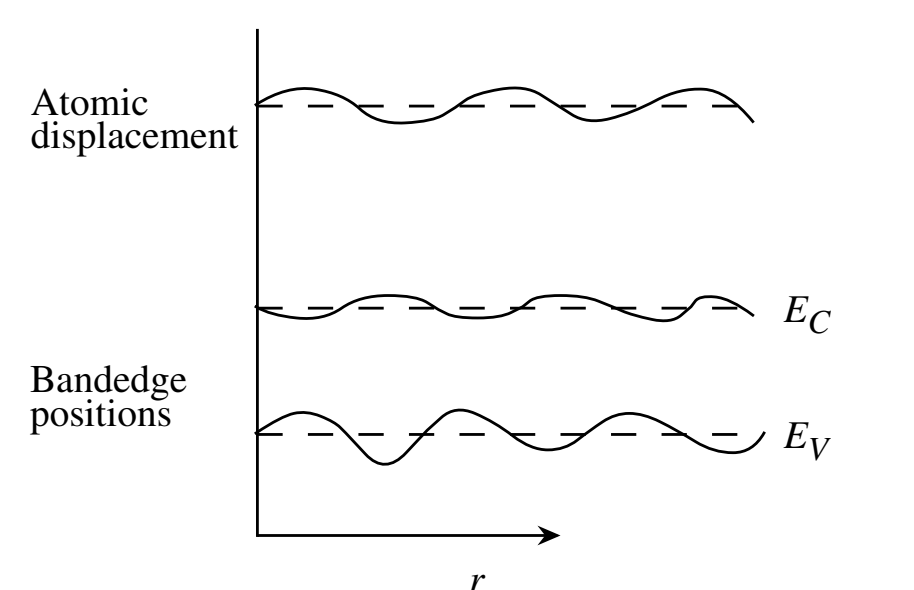
\includegraphics[width=\textwidth]{img/AtomicDisplacements.png}
		\\[0.5em]
		\refstepcounter{figure}
		\textbf{Figure~\thefigure.} Effect of atomic displacements on bandaedge energy levels in real space.
		\label{fig:AtomicDisplacements}
	\end{minipage}
\end{center}
To describe the scattering of electrons by lattice vibrations, we invoke the framework of second quantization. In this formalism, classical vibrational modes are quantized and described by phonons—quanta of vibrational energy. A harmonic oscillator with frequency $\omega$ has quantized energy levels given by
\begin{equation}
	E = \left( n + \frac{1}{2} \right) \hbar \omega
\end{equation}
where $n$ is the number of phonon quanta. The phonon number operator is defined as $n = a^\dagger a$, with $a^\dagger$ and $a$ being the phonon creation and annihilation operators, respectively. These operators satisfy the following relations:
\begin{equation}
	a |n\rangle = \sqrt{n} |n-1\rangle, \quad a^\dagger |n\rangle = \sqrt{n+1} |n+1\rangle
\end{equation}
The displacement and momentum operators in terms of $a$ and $a^\dagger$ are:
\begin{align*}
	u = \sqrt{\frac{\hbar}{2 M \omega}} (a + a^\dagger), \quad
	p = i \sqrt{\frac{M \hbar \omega}{2}} (a^\dagger - a)
\end{align*}
These expressions allow us to understand electron-phonon interactions in terms of phonon creation (emission) and annihilation (absorption) processes. In the quantum description, the emission of a phonon corresponds to the application of the creation operator, while absorption corresponds to the action of the annihilation operator.\\
Since the lattice vibrational system consists of many coupled oscillators, the physical displacement $\mathbf{u}$ representing atomic motion must be expressed in terms of normal coordinates—modes in which the vibrations are uncoupled. This transformation enables each mode to be treated as an independent harmonic oscillator. The displacement field can thus be written as
\begin{equation}
	\mathbf{u} = \frac{1}{\sqrt{N}} \sum_{\mathbf{q}} \left[\theta_{\mathbf{qb}} \mathbf{b}_\mathbf{q} e^{i \mathbf{q} \cdot \mathbf{R}}  + c.c. \right]
\end{equation}
where $q$ is the phonon wavevector, $b$ indexes the phonon branches, $\theta_b$ is the normal mode amplitude, and $N$ is the number of unit cells. This formalism provides the foundation for analyzing phonon-mediated scattering processes in semiconductors.
\begin{center}
	\begin{minipage}{0.9\textwidth}
		\centering
		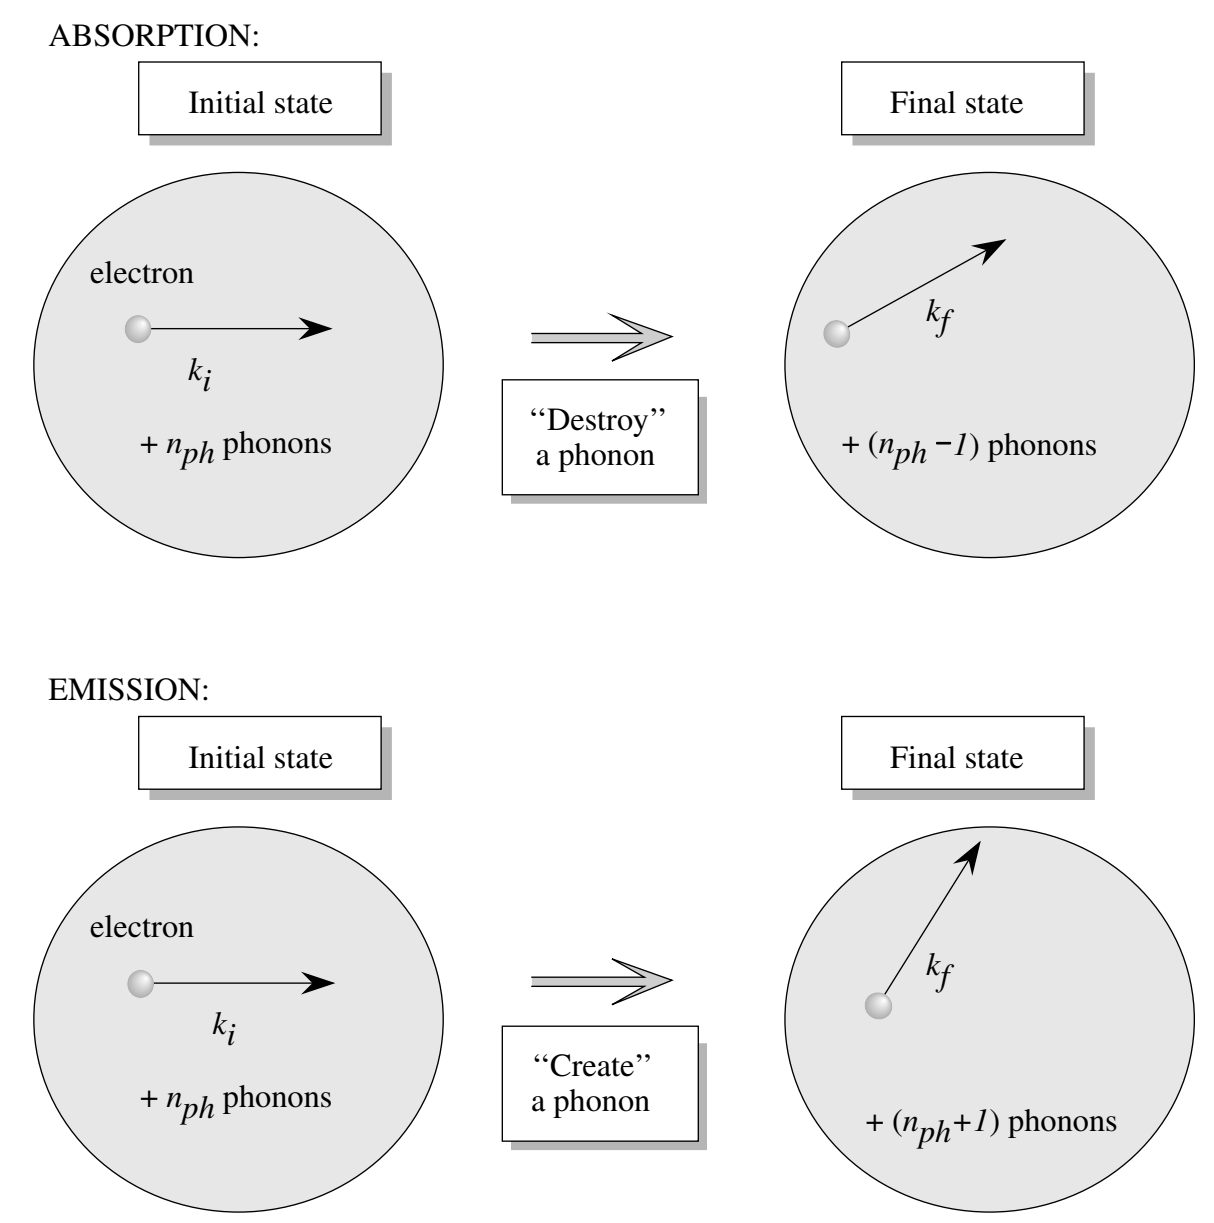
\includegraphics[width=\textwidth]{img/absandemission_phonon.png}
		\\[0.5em]
		\refstepcounter{figure}
		\textbf{Figure~\thefigure.} (a) Schematic of a phonon absorption process, where a phonon is annihilated and the electron's energy and momentum change accordingly. (b) Schematic of a phonon emission event, where a phonon is generated as the electron loses energy.
		\label{fig:absandemission_phonon}
	\end{minipage}
\end{center}

The two fundamental phonon-related processes involved in electron–phonon interactions correspond to the annihilation and creation of phonons. These are commonly referred to as \textbf{phonon absorption} and \textbf{phonon emission}, respectively.\\
In the quantum mechanical treatment of lattice vibrations, the interaction Hamiltonian includes two terms within the brackets. The first term represents the removal of a phonon from the initial state during the scattering process—this corresponds to \textbf{phonon absorption}. The second term accounts for the addition of a phonon to the final state—this is the \textbf{phonon emission} process.\\
A key distinction between the two processes arises from the phonon occupation number. Phonon absorption requires that a phonon be present initially; thus, if the initial phonon population is zero, the probability of absorption vanishes. In contrast, the emission process involves a factor of $(n + 1)$, meaning that emission can occur even in the absence of initial phonons, due to spontaneous emission.\\
At thermal equilibrium, the average phonon occupation number follows Bose–Einstein statistics.
\chapter{Optical Properties of Semiconductor}
\section{Maxwell Equations and Vector Potential}
The properties of electromagnetic fields in a medium are described by the four Maxwell equations. Apart from the electric field \( \mathbf{F} \), magnetic field \( \mathbf{B} \), and velocity of light, the effects of the material are represented by the dielectric constant \( \varepsilon \), permeability \( \mu \) (assumed \( \mu = \mu_0 \)), and electrical conductivity.
We start with the four Maxwell equations:
\begin{equation}
	\nabla \times \mathbf{F} + \frac{\partial \mathbf{B}}{\partial t} = 0, \quad
	\nabla \times \mathbf{H} - \frac{\partial \mathbf{D}}{\partial t} = \mathbf{J}, \quad
	\nabla \cdot \mathbf{D} = \rho, \quad
	\nabla \cdot \mathbf{B} = 0
\end{equation}
Here, \( \mathbf{D} = \varepsilon \mathbf{F} \), \( \mathbf{B} = \mu \mathbf{H} \), and \( \mathbf{J} \), \( \rho \) are current and charge densities, respectively.
In electron-photon interactions, it is convenient to use the scalar and vector potentials \( \phi \) and \( \mathbf{A} \), defined by:
\begin{equation}
	\mathbf{F} = -\frac{\partial \mathbf{A}}{\partial t} - \nabla \phi, \quad
	\mathbf{B} = \nabla \times \mathbf{A}
\end{equation}
These definitions automatically satisfy the first and fourth Maxwell equations. The potentials \( \phi \) and \( \mathbf{A} \) are not unique, and can be transformed using the gauge transformation:
\begin{equation}
	\mathbf{A}' = \mathbf{A} + \nabla \chi, \quad \phi' = \phi - \frac{\partial \chi}{\partial t}
\end{equation}
These transformations do not affect the physical fields \( \mathbf{F} \) and \( \mathbf{B} \).\\
Rewriting the second and third Maxwell equations in terms of \( \phi \) and \( \mathbf{A} \), we get:
\begin{equation}
	\frac{1}{\mu_0} \nabla \times (\nabla \times \mathbf{A}) + \varepsilon \frac{\partial^2 \mathbf{A}}{\partial t^2} + \varepsilon \nabla \left( \frac{\partial \phi}{\partial t} \right) = \mathbf{J}
\end{equation}
\begin{equation}
	\frac{\partial}{\partial t}(\nabla \cdot \mathbf{A}) + \nabla^2 \phi = -\frac{\rho}{\varepsilon}
\end{equation}
Using the identity:
\begin{equation}
	\nabla \times (\nabla \times \mathbf{A}) = \nabla (\nabla \cdot \mathbf{A}) - \nabla^2 \mathbf{A}
\end{equation}
We obtain:
\begin{equation}
	-\nabla^2 \mathbf{A} + \varepsilon \mu_0 \frac{\partial^2 \mathbf{A}}{\partial t^2} + \nabla \left( \nabla \cdot \mathbf{A} + \varepsilon \frac{\partial \phi}{\partial t} \right) = \mu_0 \mathbf{J}
\end{equation}
We now impose the Lorentz gauge condition:
\begin{equation}
	\nabla \cdot \mathbf{A} + \varepsilon \frac{\partial \phi}{\partial t} = 0
\end{equation}
This simplifies the Maxwell equations to:
\begin{equation}
	\nabla^2 \mathbf{A} - \varepsilon \mu_0 \frac{\partial^2 \mathbf{A}}{\partial t^2} = -\mu_0 \mathbf{J}, \quad
	\nabla^2 \phi - \varepsilon \mu_0 \frac{\partial^2 \phi}{\partial t^2} = -\frac{\rho}{\varepsilon}
\end{equation}
This form is especially useful for generalization to relativistic electrodynamics. In the **Coulomb (radiation) gauge**, where \( \mathbf{J} = 0 \) and \( \rho = 0 \), we may set \( \phi = 0 \) and \( \nabla \cdot \mathbf{A} = 0 \). The vector potential becomes a solution of the wave equation, typically:
\begin{equation}
	\mathbf{A}(\mathbf{r}, t) = \mathbf{A}_0 \left[ e^{i(\mathbf{k} \cdot \mathbf{r} - \omega t)} + \text{c.c.} \right]
\end{equation}
Where the wavevector \( \mathbf{k} \) and angular frequency \( \omega \) satisfy:
\begin{equation}
	|\mathbf{k}|^2 = \varepsilon \mu_0 \omega^2
\end{equation}
The corresponding electric and magnetic fields are:
\begin{equation}
	\mathbf{F} = -\frac{\partial \mathbf{A}}{\partial t} = 2\omega \mathbf{A}_0 \sin(\mathbf{k} \cdot \mathbf{r} - \omega t)
\end{equation}
\begin{equation}
	\mathbf{B} = \nabla \times \mathbf{A} = - 2\mathbf{k} \times \mathbf{A}_0 \sin(\mathbf{k} \cdot \mathbf{r} - \omega t)
\end{equation}
The Poynting vector representing the optical power is:
\begin{align}
	\mathbf{S} & = (\mathbf{F} \times \mathbf{H})                                                                       \\
	           & = \frac{4 v k^2}{\mu_0} \left| A_0 \right|^2 \sin^2(\mathbf{k} \cdot \mathbf{r} - \omega t) \, \hat{k}
\end{align}
The average power carried by the electromagnetic wave in the medium, where \( v = \frac{c}{\sqrt{\tilde{\epsilon}}} \) is the speed of light in the material and \( \hat{k} \) is the propagation direction unit vector, can be expressed as:
\begin{equation}
	\langle \mathbf{S} \rangle_{\text{time}} = \hat{k} \, \frac{2 v k^2 |\mathbf{A}_0|^2}{\mu_0}
\end{equation}
By rewriting the wave vector magnitude \( |\mathbf{k}| \) in terms of the angular frequency and the wave velocity, i.e.,
\begin{equation}
	|\mathbf{k}| = \frac{\omega}{v}
\end{equation}
we can substitute into the expression for the time-averaged Poynting vector to obtain:
\begin{equation}
	\langle \mathbf{S} \rangle_{\text{time}} = 2 v \epsilon \mu_0 \omega^2 |\mathbf{A}_0|^2 \hat{k}
\end{equation}
The energy stored per unit volume in the electromagnetic field can be related to the Poynting vector and the wave velocity as
\begin{equation}
	\left| \frac{S}{v} \right| = \frac{2 \epsilon \omega^2 |\mathbf{A}_0|^2}{c^2}
\end{equation}
Assuming a photon population of \( n_{\text{ph}} \), the energy density in a volume \( V \) becomes
\begin{equation}
	\frac{n_{\text{ph}} \hbar \omega}{V}
\end{equation}
Equating the two energy densities, we can isolate the amplitude of the vector potential:
\begin{equation}
	|\mathbf{A}_0|^2 = \frac{n_{\text{ph}} \hbar}{2 \epsilon \omega V}
\end{equation}
With these foundational relations established, we now consider wave propagation in a medium. By substituting \( \mathbf{J} = \sigma \mathbf{F} \) into Maxwell's equations and eliminating the magnetic field, we obtain the wave equation for the electric field:
\begin{equation}
	\nabla^2 \mathbf{F} = \epsilon \mu_0 \frac{\partial^2 \mathbf{F}}{\partial t^2} + \sigma \mu_0 \frac{\partial \mathbf{F}}{\partial t}
\end{equation}
This equation describes a damped wave. A general solution takes the form
\begin{equation}
	\mathbf{F} = \mathbf{F}_0 \exp \{ i(\mathbf{k} \cdot \mathbf{r} - \omega t) \}
\end{equation}
Substituting this into the wave equation yields the relation for the wavevector magnitude:
\begin{equation}
	-k^2 = -\epsilon \mu_0 \omega^2 - \sigma \mu_0 i \omega
\end{equation}
Or more compactly,
\begin{equation}
	k = \frac{\omega}{c} \left( \tilde{\epsilon} + \frac{\sigma \mu_0 i}{\omega} \right)^{1/2}
\end{equation}
Here, \( \tilde{\epsilon} \) represents the relative dielectric constant. In vacuum, where \( \sigma = 0 \) and \( \tilde{\epsilon} = 1 \), the wavevector simplifies to
\begin{equation}
	k = \frac{\omega}{c}
\end{equation}
Within a material, the propagation speed is affected by a complex refractive index \( n_r \), defined by
\begin{equation}
	n_r = \left( \tilde{\epsilon} + \frac{\sigma \mu_0 i}{\omega} \right)^{1/2}
\end{equation}
We can express \( n_r \) in terms of its real and imaginary parts as
\begin{equation}
	n_r = n_r' + i n_r''
\end{equation}
Substituting this into the expression for \( k \), we obtain
\begin{equation}
	k = \frac{n_r' \omega}{c} + i \frac{n_r'' \omega}{c}
\end{equation}
The electric field wave for propagation in the \( +z \) direction can be written as

\begin{equation}
	\mathbf{F} = \mathbf{F}_0 \exp\left\{ i\omega \left( \frac{n_r' z}{c} - t \right) \right\} \exp\left( \frac{-n_r'' \omega z}{c} \right)
\end{equation}
Here, the phase velocity is reduced by a factor \( n_r' \), making it \( c / n_r' \), and the wave amplitude decays exponentially as \( \exp(-2\pi n_r'' / n_r') \) per wavelength. This decay in amplitude is a result of absorption of the electromagnetic energy.\\
The absorption coefficient \( \alpha \), which characterizes the intensity loss, is given by
\begin{equation}
	\alpha = \frac{2 n_r'' \omega}{c}
\end{equation}
In the special case where there is no absorption, the real part of the refractive index \( n_r' \) equals the total refractive index \( n_r \), and \( n_r'' = 0 \).\\
The absorption coefficient is measurable and provides direct information about the imaginary component \( n_r'' \) of the refractive index.\\
The interaction of the medium with the electromagnetic field is fully described by a complex dielectric constant or equivalently a complex refractive index. The real and imaginary parts of the dielectric constant \( \tilde{\epsilon} \) are related to the refractive index components as follows:
\begin{equation}
	\tilde{\epsilon}_1 = n_r'^2 - n_r''^2, \qquad
	\tilde{\epsilon}_2 = 2 n_r' n_r''
\end{equation}
These expressions relate the real (\( \tilde{\epsilon}_1 \)) and imaginary (\( \tilde{\epsilon}_2 \)) parts of the relative permittivity to the components of the complex refractive index.\\
A very significant relationship exists between the real and imaginary parts of the refractive index based on causality—this is known as the Kramers–Kronig relation. It connects the frequency-dependent refractive index to the absorption coefficient via
\begin{equation}
	n(\omega_0) - 1 = \frac{c}{\pi} \mathcal{P} \int_0^\infty \frac{\alpha(\omega)}{\omega^2 - \omega_0^2} \, d\omega
\end{equation}
This formulation is powerful as it enables the calculation of the refractive index if the absorption coefficient is known. In cases where the absorption spectrum varies under external influences (e.g., electric fields), changes in the refractive index can be predicted accordingly.


\section{Electrons in Electromagnetic Field}
Electrons, possessing a negative charge, interact with electric and magnetic fields originating from electromagnetic radiation. The electric field exerts a force equal to the product of the charge and the field itself, whereas the magnetic field contributes through the Lorentz force, which involves the cross product between the electron's velocity and the magnetic field.\\
This interaction energy defines the interaction Hamiltonian, which plays a central role in electron scattering processes. The total Hamiltonian for a charge \( e \) in the presence of an electromagnetic field is
\begin{equation}
	H = \frac{1}{2m_0} (\mathbf{p} - e \mathbf{A})^2 + e \phi + V(\mathbf{r})
\end{equation}
Expanding the square and rearranging terms:
\begin{equation}
	H = \frac{\mathbf{p}^2}{2m_0} - \frac{e}{2m_0} (\mathbf{p} \cdot \mathbf{A} + \mathbf{A} \cdot \mathbf{p}) + \frac{e^2}{2m_0} \mathbf{A}^2 + e \phi + V(\mathbf{r})
\end{equation}
In this expression, \( \mathbf{A} \) denotes the vector potential and \( V(\mathbf{r}) \) represents any potential due to the crystal lattice.\\
Within the framework of quantum mechanics, the momentum operator \( \mathbf{p} \) is defined differentially. Therefore, the operator form of \( \mathbf{p} \cdot \mathbf{A} \) becomes
\begin{equation}
	\frac{e}{2m_0} \mathbf{p} \cdot \mathbf{A} = \frac{e}{2m_0} \mathbf{A} \cdot \mathbf{p} - \frac{i e \hbar}{2m_0} \nabla \cdot \mathbf{A}
\end{equation}
Substituting this result into the Hamiltonian yields
\begin{equation}
	H = \frac{\mathbf{p}^2}{2m_0} - \frac{e}{m_0} \mathbf{A} \cdot \mathbf{p} + \frac{i e \hbar}{2m_0} \nabla \cdot \mathbf{A} + \frac{e^2}{2m_0} \mathbf{A}^2 + e \phi + V(\mathbf{r})
\end{equation}
To analyze the influence of electromagnetic radiation on an electron, we apply perturbation theory. In the quantum mechanical description of radiation, the electromagnetic field is represented using creation and annihilation operators, akin to those used in harmonic oscillator problems—similar to the formalism previously applied to phonon interactions.\\
The time-dependent Schrödinger equation describing this system is then:
\begin{equation}
	i \hbar \frac{\partial \psi}{\partial t} = \left[
		- \frac{\hbar^2}{2m_0} \nabla^2
		+ \frac{i e \hbar}{m_0 c} \mathbf{A} \cdot \nabla
		+ \frac{i e \hbar}{2 m_0} (\nabla \cdot \mathbf{A})
		+ \frac{e^2}{2 m_0} \mathbf{A}^2
		+ e \phi + V(\mathbf{r})
		\right] \psi
\end{equation}
We adopt the radiation gauge, where \( \nabla \cdot \mathbf{A} = \phi = 0 \), and use time-dependent perturbation theory to compute scattering rates using Fermi’s golden rule. Assuming the optical power is modest, the vector potential \( \mathbf{A} \) remains small, so we can estimate:
\begin{equation}
	\left| \frac{i e \hbar}{m_0} \mathbf{A} \cdot \nabla \right| : \left| \frac{\hbar^2}{2m_0} \nabla^2 \right| \approx \left| \frac{e^2 A^2}{2m_0^2} \right| : \left| \frac{i e \hbar}{m_0} \mathbf{A} \cdot \nabla \right| \approx \frac{eA}{p}
\end{equation}
For an optical intensity of 1 W/cm\(^2\), the corresponding photon density at 1 eV energy is approximately \( 10^9 \,\text{cm}^{-3} \). With an electron velocity of \( 10^6 \,\text{cm/s} \), we find:
\begin{equation}
	\frac{eA}{p} \sim 10^{-5}
\end{equation}
This implies that even for a beam as intense as 1 MW/cm\(^2\), the quantity \( eA/p \) remains sufficiently small for perturbation theory to be applicable. Therefore, we will only consider terms linear in \( \mathbf{A} \).\\
The time-dependent Schrödinger equation now simplifies to:
\begin{equation}
	i \hbar \frac{\partial \psi}{\partial t} = (H_0 + H') \psi
\end{equation}
where the unperturbed Hamiltonian is:
\begin{equation}
	H_0 = -\frac{\hbar^2}{2m_0} \nabla^2 + V(\mathbf{r})
\end{equation}
and the perturbation is given by:
\begin{equation}
	H' = \frac{i e \hbar}{m_0} \mathbf{A} \cdot \nabla
\end{equation}
\begin{center}
	\begin{minipage}{0.8\textwidth}
		\centering
		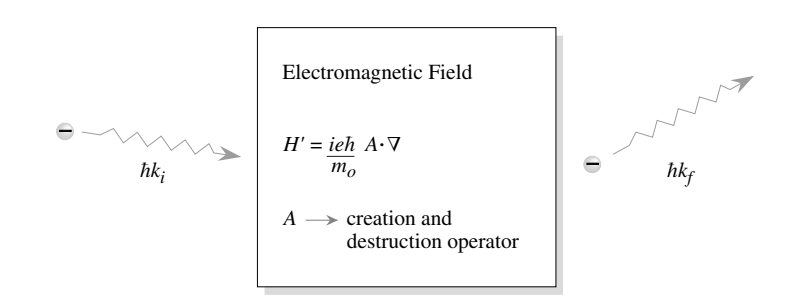
\includegraphics[width=\textwidth]{img/Scattering.png}
		\\[0.5em]
		\refstepcounter{figure}
		\textbf{Figure~\thefigure.} Schematic of the scattering process of an electron by the electromagnetic field.
		\label{fig:Scattering}
	\end{minipage}
\end{center}
The scattering process arises from this perturbation, where the electromagnetic field induces transitions in the electron states. In the second quantization framework, \( \mathbf{A} \) is quantized using photon creation and annihilation operators \( b^\dagger \) and \( b \), analogous to the harmonic oscillator treatment.\\
According to Fermi’s golden rule, the transition rate from an initial state \( |i\rangle \) to a final state \( |f\rangle \) is:
\begin{equation}
	W(i) = \frac{2\pi}{\hbar} \sum_f \left| \langle f | H' | i \rangle \right|^2 \delta \left( E_f - E_i \mp \hbar \omega \right)
\end{equation}
Here, the upper sign corresponds to photon absorption and the lower sign to emission.\\
The initial and final states are described by the electron's momentum and the photon number.

In the case of photon \textbf{absorption}, the states are:
\begin{align*}
	|i\rangle & = |k_i, n_{\text{ph}} \rangle     \\
	|f\rangle & = |k_f, n_{\text{ph}} - 1 \rangle
\end{align*}
\textbf{Emission:}
\begin{align*}
	|i\rangle & = |k_i, n_{\text{ph}}\rangle     \\
	|f\rangle & = |k_f, n_{\text{ph}} + 1\rangle
\end{align*}
Here, \(k_i\) and \(k_f\) denote the initial and final wavevectors of the electron, respectively, and \(n_{\text{ph}}\) is the initial photon occupation number. The vector potential \(A_0\) is defined as:
\begin{equation}
	A_0 = \sqrt{\frac{\hbar}{2 \omega \epsilon V}} \left(b^\dagger + b\right)
\end{equation}
In this expression, \(b^\dagger\) and \(b\) are the photon creation and annihilation operators. This form is chosen to be consistent with the magnitude \(|A_0|^2\) used previously.\\
When calculating matrix elements, we consider the photon operators separately. Let \( \mathbf{a} \) represent the polarization unit vector. Focusing on the matrix element due to the photon part only:
\textbf{Absorption:}
\begin{align*}
	\langle f | \mathbf{A} \cdot \nabla | i \rangle & \Rightarrow
	\sqrt{\frac{\hbar}{2 \omega \epsilon}} \left\langle k_f, n_{\text{ph}} - 1 \middle| \left(b^\dagger + b\right) \mathbf{a} \cdot \nabla \middle| k_i, n_{\text{ph}} \right\rangle             \\
	                                                & = \sqrt{\frac{\hbar}{2 \omega \epsilon}} \sqrt{n_{\text{ph}}} \left\langle k_f \middle| \mathbf{a} \cdot \nabla \middle| k_i \right\rangle
\end{align*}
\textbf{Emission:}
\begin{align*}
	\langle f | \mathbf{A} \cdot \nabla | i \rangle & \Rightarrow
	\sqrt{\frac{\hbar}{2 \omega \epsilon}} \left\langle k_f, n_{\text{ph}} + 1 \middle| \left(b^\dagger + b\right) \mathbf{a} \cdot \nabla \middle| k_i, n_{\text{ph}} \right\rangle                 \\
	                                                & = \sqrt{\frac{\hbar}{2 \omega \epsilon}} \sqrt{n_{\text{ph}} + 1} \left\langle k_f \middle| \mathbf{a} \cdot \nabla \middle| k_i \right\rangle
\end{align*}
It is crucial to notice the difference in prefactors: \( \sqrt{n_{\text{ph}}} \) appears for absorption, while \( \sqrt{n_{\text{ph}} + 1} \) appears for emission. This distinction will play a significant role in later discussions.
To proceed with calculating the rate for photon absorption—where a photon of energy \(\hbar \omega\) and momentum \(\hbar k_{\text{ph}}\) is absorbed by an electron—we will need to sum over all possible electron states which can allow such a process to occur.\\
\begin{center}
	\begin{minipage}{0.5\textwidth}
		\centering
		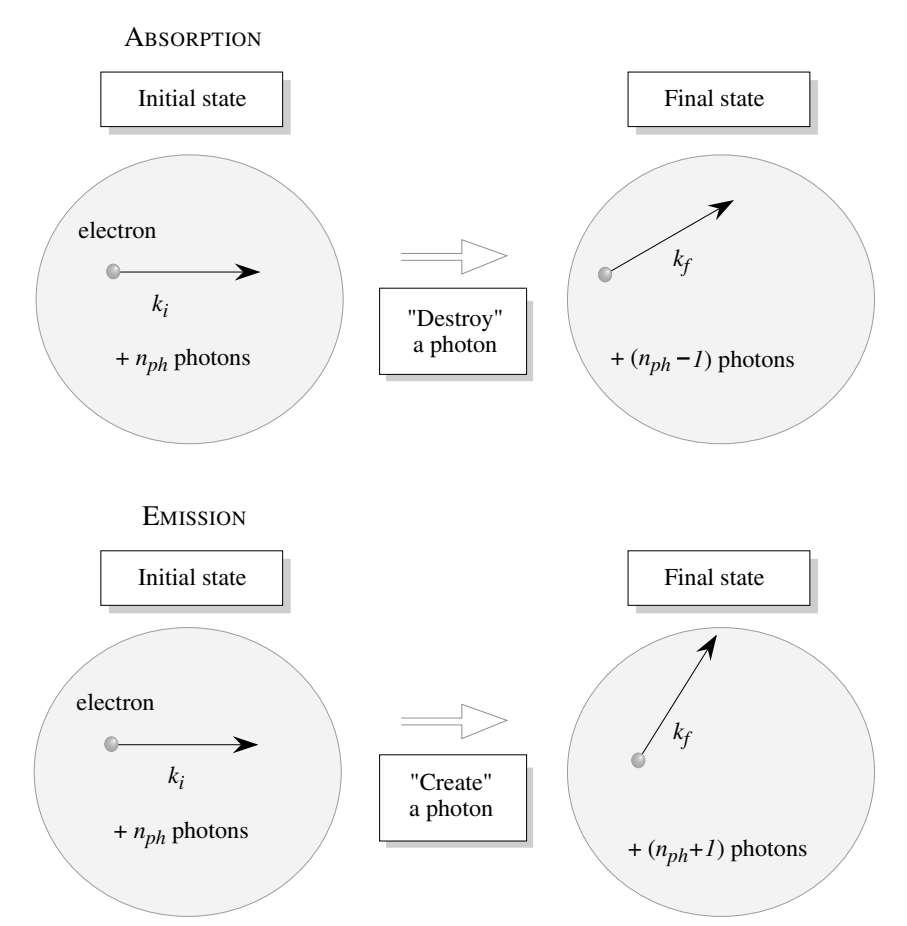
\includegraphics[width=\textwidth]{img/Abs&emiss.png}
		\\[0.5em]
		\refstepcounter{figure}
		\textbf{Figure~\thefigure.} (a) Schematic of a photon absorption process, where a photon is annihilated and the electron’s energy and momentum change.  
(b) Photon emission process, where a photon is generated as the electron transitions to a lower energy state. 
		\label{fig:Abs&emiss}
	\end{minipage}
\end{center}
The process of photon absorption involves the transfer of photon energy \(\hbar \omega\) to an electron. To compute the full scattering rate, we integrate over the final electron density of states:
\begin{equation}
W_{\text{abs}} = \frac{2\pi}{\hbar} \frac{e^2}{m_0^2} \left( \frac{\hbar n_{\text{ph}}}{2 \omega \epsilon} \right) \sum_{\text{final states}} \left| \int \psi_f^* (\mathbf{a} \cdot \mathbf{p}) e^{i \mathbf{k}_{\text{ph}} \cdot \mathbf{r}} \psi_i \, d^3r \right|^2 \delta(E_i - E_f + \hbar \omega)
\end{equation}
This expression includes a sum over all possible electronic final states for photon absorption, ensuring energy conservation. Alternatively, one might be interested in electron scattering from an initial state with momentum \(k_i\) to a final state with momentum \(k_f\), summing instead over photon states that enable this transition.\\
For photon emission, where an electron in state \(\hbar k_i\) emits a photon and transitions to \(\hbar k_f\), the corresponding rate is:
\begin{equation}
W_{\text{em}} = \frac{2\pi}{\hbar} \frac{e^2}{m_0^2} \left( \frac{\hbar(n_{\text{ph}} + 1)}{2 \omega \epsilon} \right) \sum_{\text{final states}} \left| \int \psi_f^* (\mathbf{a} \cdot \mathbf{p}) e^{-i \mathbf{k}_{\text{ph}} \cdot \mathbf{r}} \psi_i \, d^3r \right|^2 \delta(E_i - E_f - \hbar \omega)
\end{equation}
This emission rate can be broken into two components: one for stimulated emission and one for spontaneous emission:
\begin{equation}
W_{\text{em}} = W_{\text{st}} + W_{\text{spon}}
\end{equation}
where
\begin{equation}
W_{\text{st}} = \frac{2\pi}{\hbar} \frac{e^2}{m_0^2} \frac{\hbar n_{\text{ph}}}{2 \omega \epsilon} \sum_{\text{final states}} \left| \int \psi_f^* e^{-i \mathbf{k}_{\text{ph}} \cdot \mathbf{r}} (\mathbf{a} \cdot \mathbf{p}) \psi_i \, d^3r \right|^2 \delta(E_i - E_f - \hbar \omega)
\end{equation}
\begin{equation}
W_{\text{spon}} = \frac{2\pi}{\hbar} \frac{e^2}{m_0^2} \frac{\hbar}{2 \omega \epsilon} \sum_{\text{final states}} \left| \int \psi_f^* e^{-i \mathbf{k}_{\text{ph}} \cdot \mathbf{r}} \psi_i \, d^3r \right|^2 \delta(E_i - E_f - \hbar \omega)
\end{equation}
\textit{Stimulated emission} arises from the presence of photons already in the system, and the emitted photons are phase coherent with the initial ones. \textit{Spontaneous emission}, on the other hand, originates from quantum vacuum fluctuations (\(n_{\text{ph}} = 0\)) and results in photons that are phase-incoherent.\\
This distinction is fundamental in understanding the operational differences between devices such as LEDs and laser diodes.\\
When examining semiconductor states, we observe that the photon momentum \(\hbar k_{\text{ph}}\), for typical photon energies between 0.1 and 2.0 eV, is much smaller than the electron momentum. Therefore, momentum conservation requires that:
\begin{equation}
k_i = k_f
\end{equation}
In first-order perturbation theory, transitions triggered by photon absorption or emission are represented as "vertical" processes in the energy–momentum (\(E\)-\(k\)) diagram. This is particularly evident in interband transitions. When the photon momentum \(k_{\text{ph}}\) is small enough to be neglected, the approximation is referred to as the dipole approximation. Under this approximation, the momentum matrix element (the integral within the absolute value bars in the relevant transition rate equations) simplifies significantly. We denote this matrix element as \(p_{if}\).\\
Let us now consider the case where both the initial and final states follow the Bloch form. In the dipole approximation, the momentum matrix element becomes:
\begin{equation}
p_{if} = -i\hbar \int \psi^*_{\mathbf{k}_f \ell'} \, \nabla \psi_{\mathbf{k}_i \ell} \, d^3 r
\end{equation}
We define the initial and final Bloch states as follows:
\[
\begin{aligned}
    |i\rangle &= \psi_{\mathbf{k}_i, \ell} = e^{i \mathbf{k}_i \cdot \mathbf{r}} u_{\mathbf{k}_i \ell}, \\
    |f\rangle &= \psi_{\mathbf{k}_f, \ell'} = e^{i \mathbf{k}_f \cdot \mathbf{r}} u_{\mathbf{k}_f \ell'},
\end{aligned}
\]
where \( u_{\mathbf{k} \ell} \) denotes the cell-periodic part of the Bloch wavefunction, and \(\ell\), \(\ell'\) are band indices.\\
By applying the gradient operator to the initial state, the momentum matrix element simplifies into the following form:
\begin{equation}
p_{if} = \hbar \mathbf{k}_i \int \psi^*_{\mathbf{k}_f \ell'} \psi_{\mathbf{k}_i \ell} \, d^3 r 
- i\hbar \int u^*_{\mathbf{k}_f \ell'} \left( \nabla u_{\mathbf{k}_i \ell} \right) 
e^{i(\mathbf{k}_i - \mathbf{k}_f) \cdot \mathbf{r}} \, d^3 r
\end{equation}
\begin{figure}[H]
    \centering
    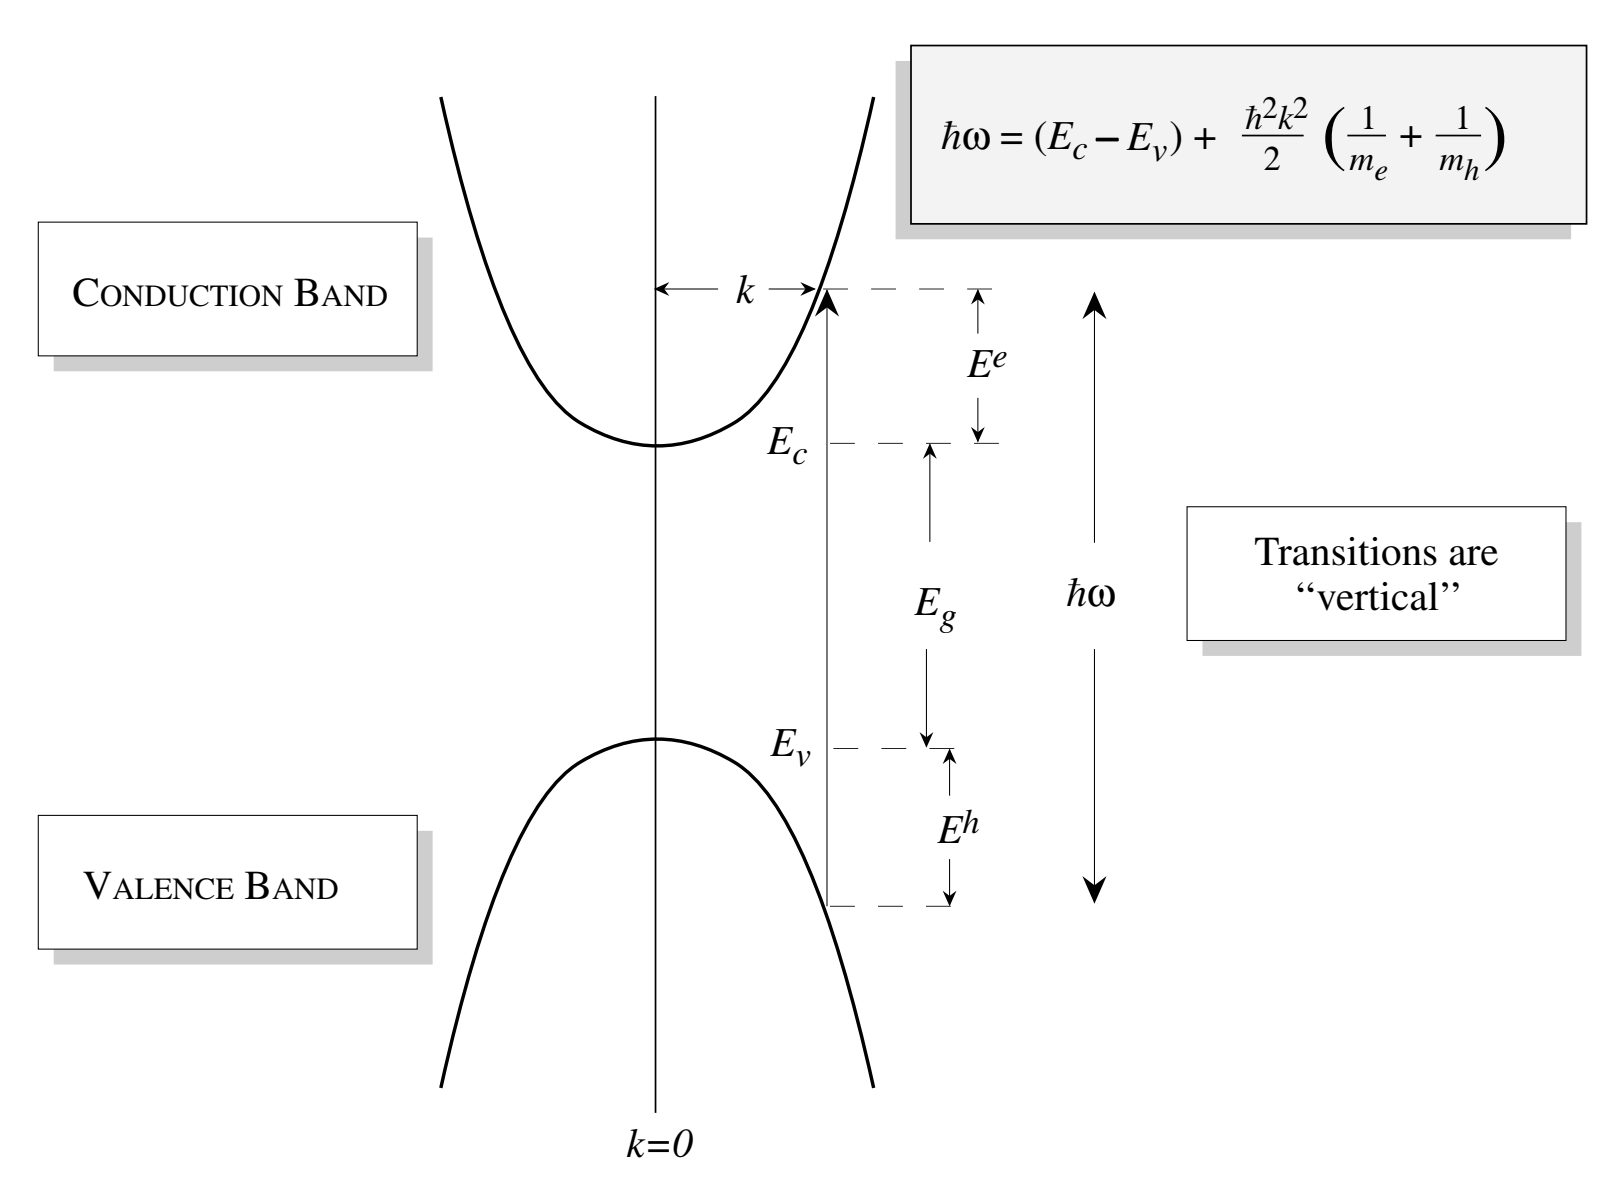
\includegraphics[width=0.8\textwidth]{img/transitions.png}
    \caption{Electron and hole energy levels at vertical \(\mathbf{k}\)-values. The transition energies are set by the photon energy and the effective masses of the carriers. Due to the negligible photon momentum, these transitions occur vertically in \(\mathbf{k}\)-space.
    }
    \label{fig:transitions}
\end{figure}



\section{Interband Transitions}

\subsection{Interband Transitions in Bulk Semiconductors}
\subsection{Interband Transitions in Quantum Wells}



\section{Indirect Interband Transitions}


\section{Intraband Transitions}
\subsection{Intraband Transitions in Bulk Semiconductors}
\subsection{Intraband Transitions in Quantum Wells}



\section{Charge Injection and Radiative Recombination}
\subsection{Spontaneous Emission Rate}
\subsection{Gain in a Semiconductor}



\section{Nonradiative Recombination}
\subsection{Charge Injection: Nonradiative Effects}
\subsection{Non-radiative Recombination: Auger Process}


\section{Semiconductor Light Emitters}
\subsection{Light Emitting Diode}
\subsection{Laser Diode}
\subsubsection{Optical Absorption, Loss and Gain}
\subsubsection{Laser Below and Above Threshold}
\chapter{Excitonic Effects}
\section{Introduction}
The bandstructure and optical properties of semiconductors discussed so far have been based on the assumption that the valence band is completely filled with electrons while the conduction band remains empty. Under this assumption, the effects of carriers—electrons in the conduction band and holes in the valence band—enter only through the occupation probabilities, without altering the underlying bandstructure.\\
In practice, however, there exists a Coulombic interaction between electrons and other charged carriers, such as additional electrons or holes. These interactions can lead to significant modifications in material properties. Let us now consider a situation in which a single electron occupies the conduction band, while a corresponding hole is present in the valence band. This configuration introduces a direct Coulomb attraction between the electron and hole, altering the Hamiltonian of the system.\\
The resultant electron–hole pair, bound by this Coulomb interaction, forms a new quasiparticle known as an exciton. The formation of an exciton necessitates a re-evaluation of the electronic bandstructure to incorporate the effects of this binding.\\
The study of excitonic transitions in quantum wells has emerged as a major area of research, driven by both fundamental physics and technological applications. In quantum confined systems, the exciton binding energy is significantly enhanced compared to bulk materials. Additionally, the strength of optical transitions is improved, leading to the observation of sharp resonance features in the optical spectra of quantum wells. These excitonic resonances are highly tunable using optical or electronic methods, making them especially valuable in device applications.\\
Modulation of optical properties is a critical component in the development of advanced optoelectronic technologies. Although several types of external stimuli—such as electric fields, magnetic fields, and mechanical strain—can influence the optical response of a material, only modulation by electric or electromagnetic fields can achieve high-speed performance. In bulk semiconductors, the modulation capabilities are generally limited. However, quantum wells exhibit markedly enhanced modulation behavior, which makes them ideal candidates for integrated photonic and optoelectronic systems.\\
In this chapter, we will explore the physical principles underlying various approaches to optical modulation, with a particular focus on quantum-confined systems.


\section{Excitonic States in Semiconductors}
The electron–hole pair forms a bound state that can be described by an envelope function. This envelope function, representing the spatial distribution of the bound state, can be derived by treating the Coulombic interaction between the electron and hole as a perturbation.\\
There are two major categories of excitons, distinguished by the spatial extent of their envelope functions. When the envelope function is confined to only a few unit cells, the exciton is referred to as a Frenkel exciton. Owing to their highly localized nature, the Heisenberg uncertainty principle implies that such excitons require a treatment that incorporates the full electronic bandstructure of the material.\\
These localized excitons contrast with another class—commonly encountered in semiconductors—where the envelope function is much more extended. Each class of exciton gives rise to different optical and transport properties and must be described using appropriate theoretical frameworks.
\begin{center}
	\begin{minipage}{0.8\textwidth}
		\centering
		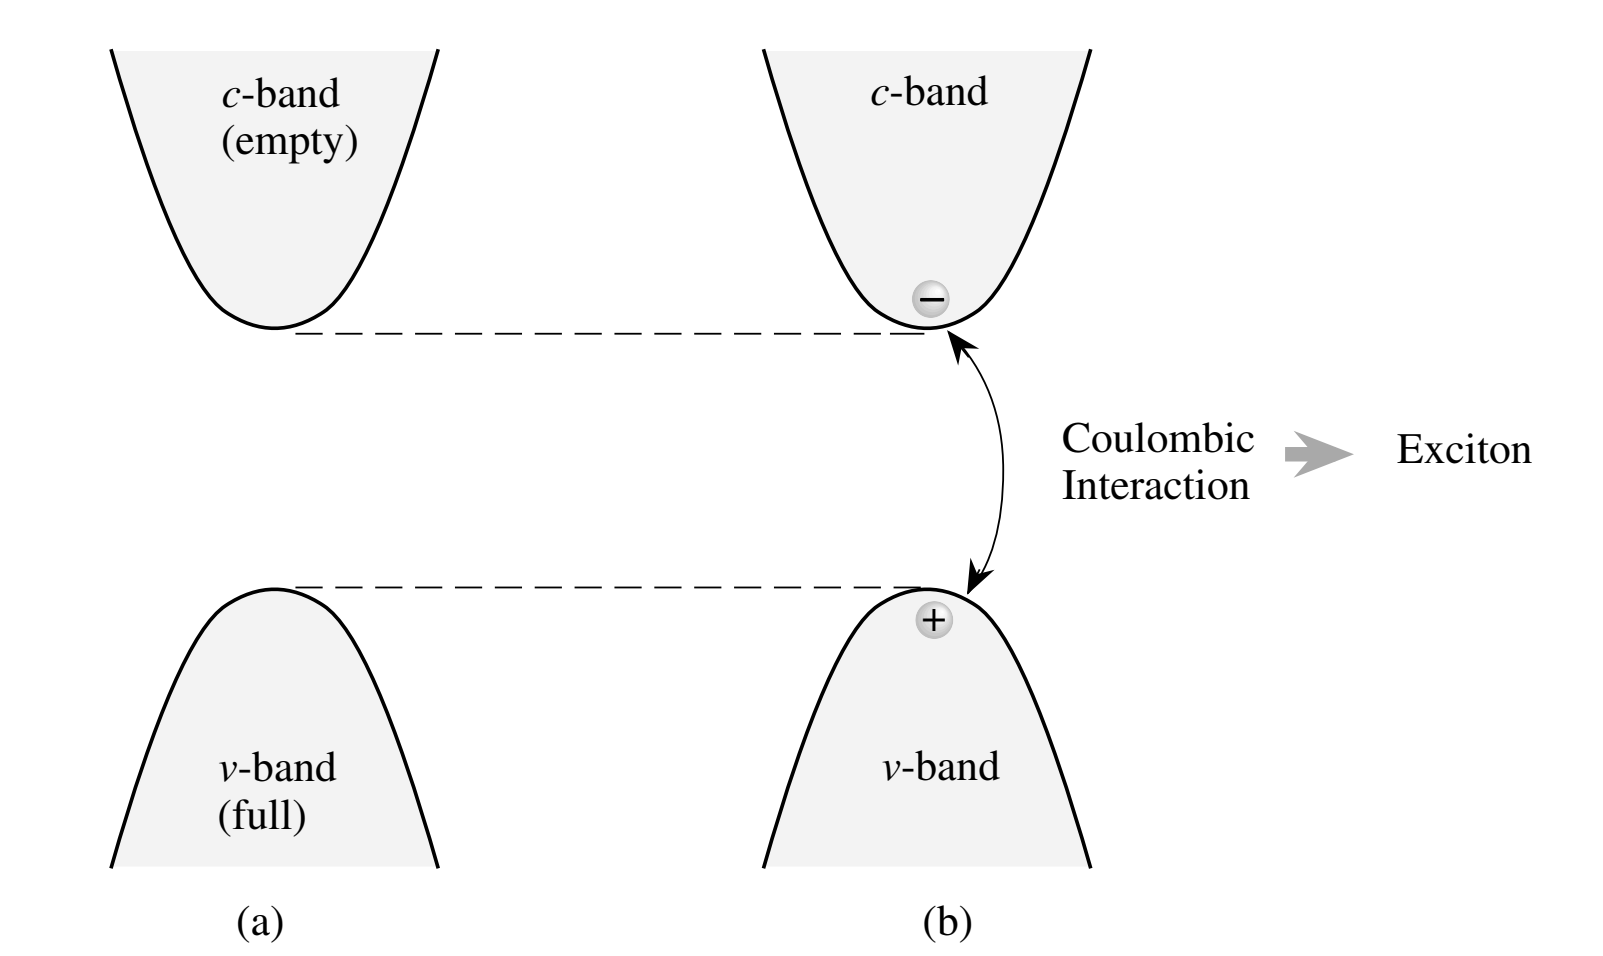
\includegraphics[width=\textwidth]{img/hole_interaction.png}
		\\[0.5em]
		\refstepcounter{figure}
		\textbf{Figure~\thefigure.} (a) Bandstructure under the independent electron approximation.
		(b) Modification of the bandstructure due to Coulomb interaction between an electron and a hole.
		\label{fig:hole_interaction}
	\end{minipage}
\end{center}
\begin{center}
	\begin{minipage}{0.75\textwidth}
		\centering
		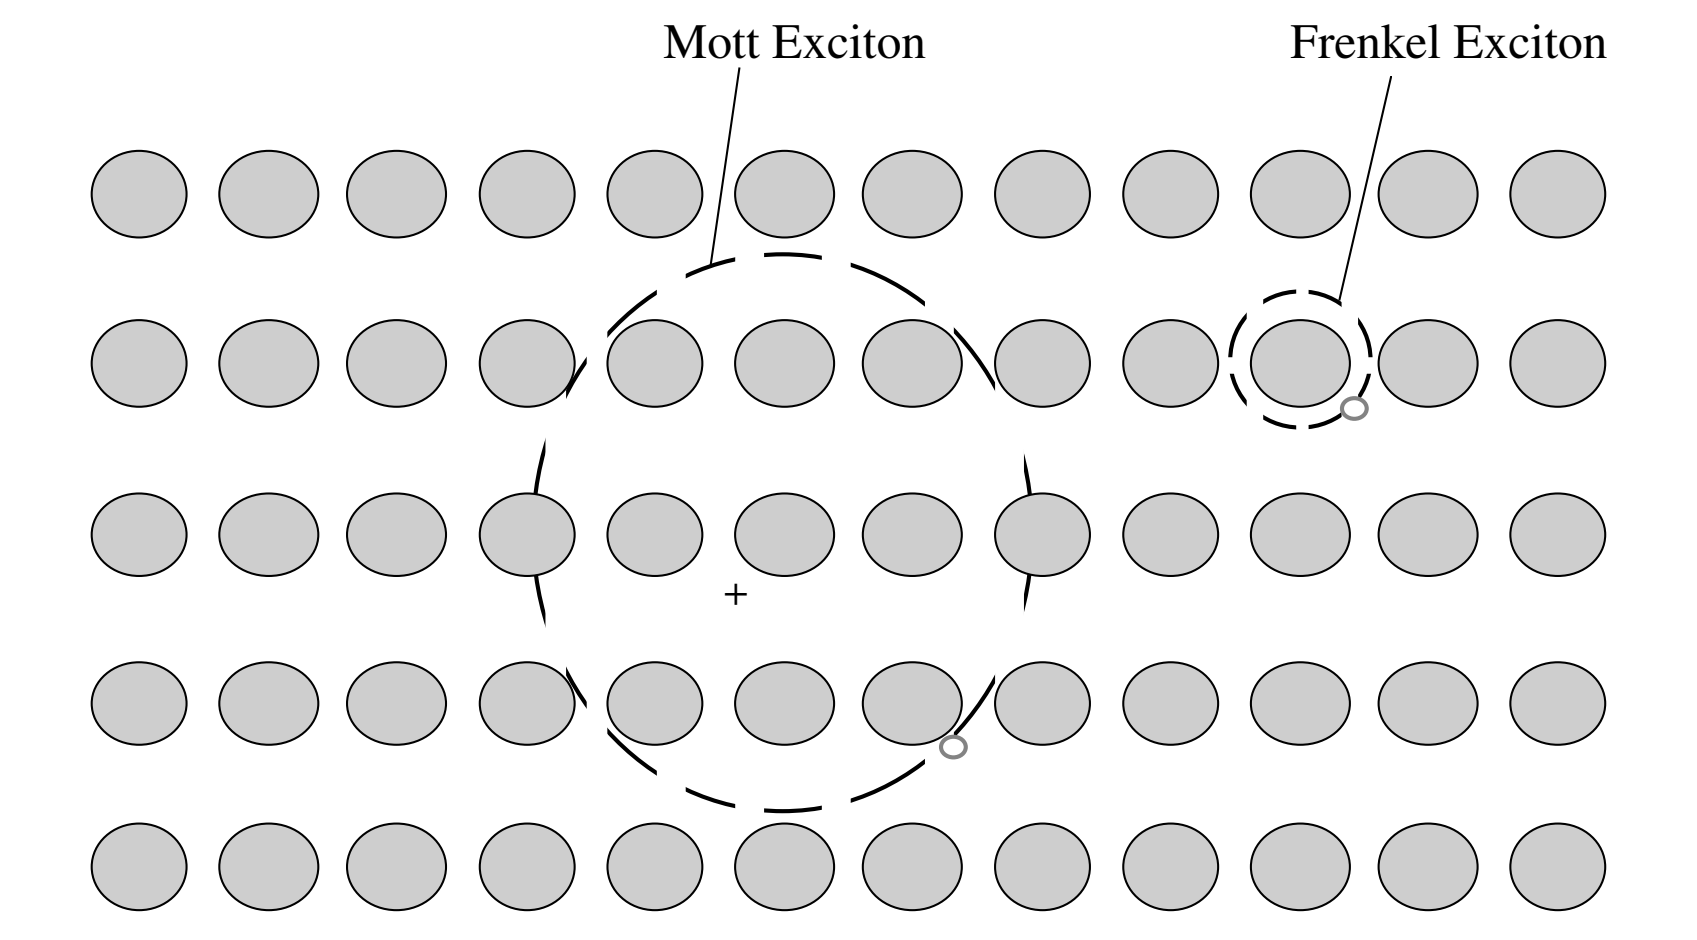
\includegraphics[width=\textwidth]{img/exciton.png}
		\\[0.5em]
		\refstepcounter{figure}
		\textbf{Figure~\thefigure.} Conceptual illustration of the periodic envelope functions of Frenkel and Mott excitons. The Frenkel exciton is localized over a few unit cells, while the Mott exciton extends across many unit cells.
		\label{fig:exciton}
	\end{minipage}
\end{center}

Such excitons, which arise when the electron and hole form a spatially extended bound state, are referred to as Mott excitons. These excitons are central to the excitonic physics in semiconductors. Their properties can be described using the effective mass approximation, whereby the electron–hole interaction is incorporated into a modified Schrödinger equation of the form:
\begin{equation}
	\left[- \frac{\hbar^2}{2m_e^*} \nabla_e^2 - \frac{\hbar^2}{2m_h^*} \nabla_h^2 - \frac{e^2}{4\pi \varepsilon | \mathbf{r}_e - \mathbf{r}_h |} \psi_{ex} \right] = E \psi_{ex}
\end{equation}
Here, \( m_e^* \) and \( m_h^* \) are the effective masses of the electron and hole, respectively, and \( |\mathbf{r}_e - \mathbf{r}_h| \) denotes the distance between the electron and hole, which determines the strength of their Coulomb interaction. \( E_{\text{ex}} \) is the energy of the exciton.
This formulation presents a two-body problem, which can be simplified by transforming to center-of-mass and relative coordinates:
\begin{equation}
	\mathbf{r} = \mathbf{r}_e - \mathbf{r}_h, \quad \mathbf{R} = \frac{m_e^* \mathbf{r}_e + m_h^* \mathbf{r}_h}{m_e^* + m_h^*}
\end{equation}
and corresponding wavevectors:
\begin{equation}
	\mathbf{k} = \frac{m_e^* \mathbf{k}_e + m_h^* \mathbf{k}_h}{m_e^* + m_h^*}, \quad \mathbf{K} = \mathbf{k}_e + \mathbf{k}_h
\end{equation}
The total Hamiltonian can then be written as:
\begin{equation}
	H = \frac{\hbar^2 K^2}{2(m_e^* + m_h^*)} +  \left( \frac{\hbar^2 k^2}{2 m_r^*} - \frac{e^2}{4\pi \varepsilon |\mathbf{r}|} \right)
\end{equation}
The Hamiltonian consists of two parts: the first term describes the center-of-mass motion, which leads to a plane-wave solution:
\begin{equation}
	\psi_{\text{cm}}(\mathbf{R}) = e^{i \mathbf{K} \cdot \mathbf{R}}
\end{equation}
The second term describes the relative motion of the electron–hole pair. Its solution satisfies:
\begin{equation}
	\left[ - \frac{\hbar^2 k^2}{2m_r^*} - \frac{e^2}{4\pi \varepsilon |\mathbf{r}|} \right] F(\mathbf{r}) = E_n F(\mathbf{r})
\end{equation}
This equation is analogous to the hydrogen atom problem, and its solutions \( F(\mathbf{r}) \) are hydrogen-like wavefunctions. The full exciton wavefunction is then:
\begin{equation}
	\psi_{n,\mathbf{K}_{ex}}(\mathbf{r}_e, \mathbf{r}_h) = e^{i \mathbf{K}_{ex} \cdot \mathbf{R}} F_n(\mathbf{r}) \phi_c(\mathbf{r}_e) \phi_v(\mathbf{r}_h)
\end{equation}
Here, \( \phi_c \) and \( \phi_v \) represent the Bloch functions of the conduction and valence band edge states, respectively. The corresponding excitonic energy levels are given by:
\begin{equation}
	E_{n,\mathbf{K}_{ex}} = E_n + \frac{\hbar^2}{2(m_e^* + m_h^*)} K_{ex}^2
\end{equation}
where the eigenvalues \( E_n \) are:
\begin{equation}
	E_n = - \frac{m_r^* e^4}{2 (4 \pi \varepsilon)^2 \hbar^2 n^2}, \quad n = 1, 2, 3, \dots
\end{equation}
The quantity \( E_n \) is measured relative to the conduction band minimum, i.e., the excitonic energy levels appear just below the bandgap. Typical binding energies for excitons in semiconductors range from approximately 2 to 6~meV.\\
This modified dispersion relation, which includes the Coulomb interaction, differs from the conventional energy–wavevector (\( E \) vs.\ \( k \)) relationship. Since the exciton is a composite particle, the appropriate quantum number is not the electron or hole momentum individually, but the total crystal momentum \( \mathbf{K} \) of the electron–hole pair. When the Coulomb interaction is neglected, the bound-state energy levels vanish, and one recovers the usual free electron–hole dispersion relation.\\
A key consequence of excitonic formation is that, unlike in free-carrier models where the joint density of states begins at the band edge, the presence of excitons introduces a density of states below the bandgap. Nevertheless, due to momentum conservation, not all exciton states will couple effectively to photons.
\begin{center}
	\begin{minipage}{0.6\textwidth}
		\centering
		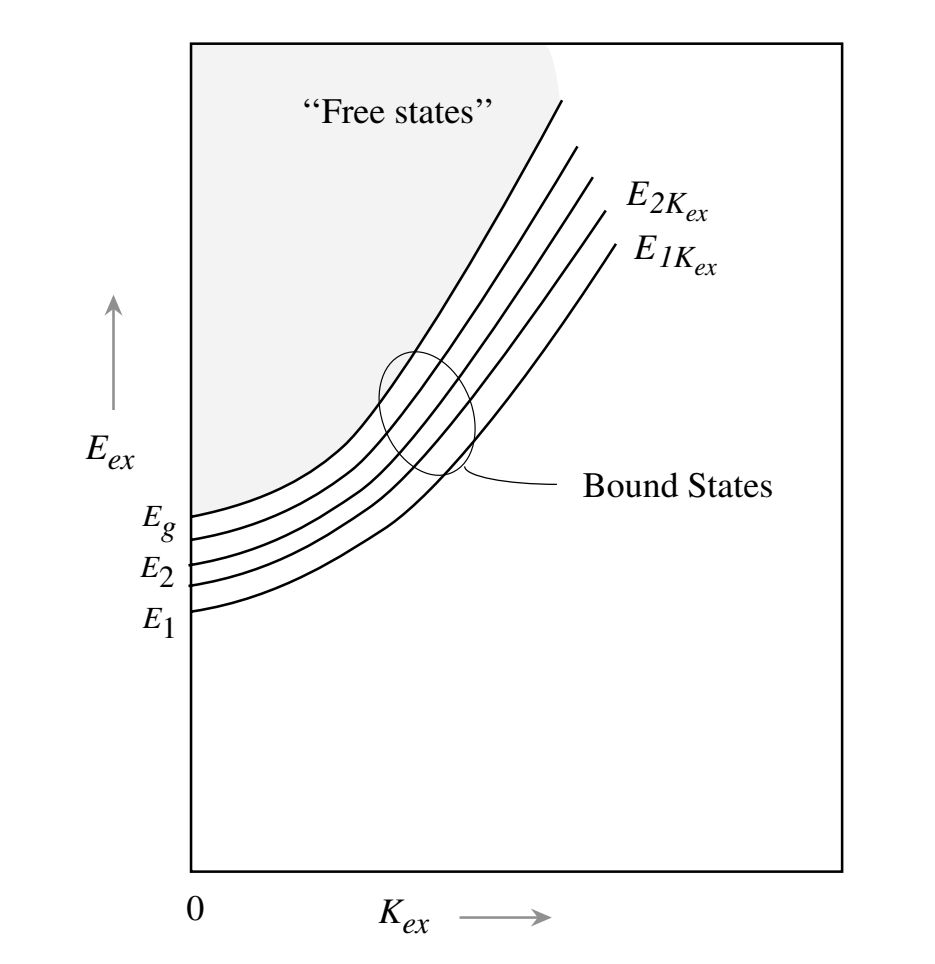
\includegraphics[width=\textwidth]{img/Dispersion_curves.png}
		\\[0.5em]
		\refstepcounter{figure}
		\textbf{Figure~\thefigure.} Dispersion curves for the electron-hole system in the exciton framework
		\label{fig:Dispersion_curves}
	\end{minipage}
\end{center}
To analyze the absorption spectra of excitonic transitions in semiconductors, it is useful to examine the problem in greater detail. As previously discussed, the independent-electron model yields the conduction and valence band states. When electron–hole pairs are introduced, their mutual Coulomb interaction can be treated as a perturbation. The resulting excitonic wavefunction can then be expressed as a linear combination of the independent electron basis functions.\\
The general form of the excitonic Hamiltonian is given by:
\begin{equation}
	H = H_0 + \frac{1}{2} \sum_{i \neq j} \frac{e^2}{4\pi \varepsilon_0 |\mathbf{r}_i - \mathbf{r}_j|}
\end{equation}
Here, \( H_0 \) is the unperturbed Hamiltonian representing the independent electron bandstructure, and the second term accounts for the Coulomb interactions between different electrons. The factor of \( \frac{1}{2} \) prevents double counting. Indices \( i \) and \( j \) label individual particles.\\
Because the full Hamiltonian maintains the symmetry of the underlying crystal lattice, the Bloch theorem remains applicable. Therefore, the total excitonic wavefunction must satisfy:
\begin{equation}
	\psi_{\text{ex}}(\mathbf{r}_1 + \mathbf{R}, \mathbf{r}_2 + \mathbf{R}, \dots) = e^{i\mathbf{K} \cdot \mathbf{R}} \psi_{\text{ex}}(\mathbf{r}_1, \mathbf{r}_2, \dots)
\end{equation}
where \( \mathbf{R} \) is a lattice vector and \( \mathbf{K} \) is the total crystal momentum of the exciton.
The exciton state can be written in terms of a basis function \( \Phi_{c,\mathbf{k_e}, S_e; v,\mathbf{k_h}, S_h} \), which represents a conduction band state where an electron, with momentum \(\mathbf{k}_e\) and spin \(S_e\) in the conduction band, and a valence band hole with momentum \(\mathbf{k}_h\) and spin \(S_h\). The difference \( \mathbf{k}_e - \mathbf{k}_h \) is equal to the total momentum \( \mathbf{K} \) of the exciton.\\
The exciton wavefunction is expressed as:
\begin{equation}
	\psi_{\text{ex}}^{n,\ell,m} = \sum_{\mathbf{k}} A_{n,\ell,m}(\mathbf{k}) \Phi^{n,\ell,m}_{c,\mathbf{k}+\mathbf{K}_{ex}/2,S_e; v,\mathbf{k}-\mathbf{K}_{ex}/2,S_h}
\end{equation}
Here, \( n \), \( \ell \), and \( m \) are quantum numbers associated with the exciton state, and \( A_{n,\ell,m}(\mathbf{k}) \) are expansion coefficients. Since we are dealing with envelope functions that are spatially extended (on the order of 100~\AA), the expansion coefficients are expected to be sharply localized in momentum space.\\
We can define the Fourier transform of \( A_{n,\ell,m}(\mathbf{k}) \) as the real-space envelope function:
\begin{equation}
	F_{n,\ell,m}(\mathbf{r}) = \sum_{\mathbf{k}} A_{n,\ell,m}(\mathbf{k}) e^{i \mathbf{k} \cdot \mathbf{r}}
\end{equation}
This function satisfies a Schrödinger-like equation, analogous to the hydrogen atom, but modified for the semiconductor environment:
\begin{equation}
	\left[ E_{cv}(-i\nabla, \mathbf{K}_{ex}) - \frac{e^2}{4\pi \varepsilon \mathbf{r}} \right] F_{n,\ell,m}(\mathbf{r}) = E_{\text{ex}} F_{n,\ell,m}(\mathbf{r})
\end{equation}
Here, \( E_{cv}(-i\nabla, \mathbf{K}_{ex}) \) results from expanding the difference \( E_c(\mathbf{k} + \mathbf{K}_{ex}/2) - E_v(\mathbf{k} - \mathbf{K}_{ex}/2) \) in powers of \( \mathbf{k} \) and substituting \( \mathbf{k} \rightarrow -i\nabla \). Exchange interactions are typically negligible and are therefore omitted. At low carrier densities, the dielectric constant \( \varepsilon \) can be approximated by its static value.\\
For a simple parabolic band structure, the exciton binding energy levels are:
\begin{equation}
	E^{\text{ex}}_n = E_g - \frac{m_r^*e^4}{2(4\pi \varepsilon)^2 \hbar^2 n^2} = E_g - \frac{R_{\text{ex}}}{n^2}
\end{equation}
where \( m_r^* \) is the reduced mass of the electron–hole pair and \( R_{\text{ex}} \) is the exciton Rydberg. The kinetic energy associated with the center-of-mass motion of the exciton should be added to this expression for the total energy.\\
The corresponding envelope functions are hydrogen-like. For example, the ground state wavefunction is:
\begin{equation}
	F_{100}(\mathbf{r}) = \frac{1}{\sqrt{\pi a_{\text{ex}}^3}} e^{-r/a_{\text{ex}}}
\end{equation}
with the exciton Bohr radius given by:
\begin{equation}
	a_{\text{ex}} = \frac{\varepsilon m_0}{\varepsilon_0 m_r^*} a_B, \quad \text{where } a_B = 0.529\,\text{\AA}
\end{equation}
For most semiconductors, \( a_{\text{ex}} \) is on the order of 100~\AA, indicating that the exciton is spread over many unit cells. This justifies the use of the effective mass approximation in the description of such extended excitonic states.
\begin{center}
	\begin{minipage}{0.8\textwidth}
		\centering
		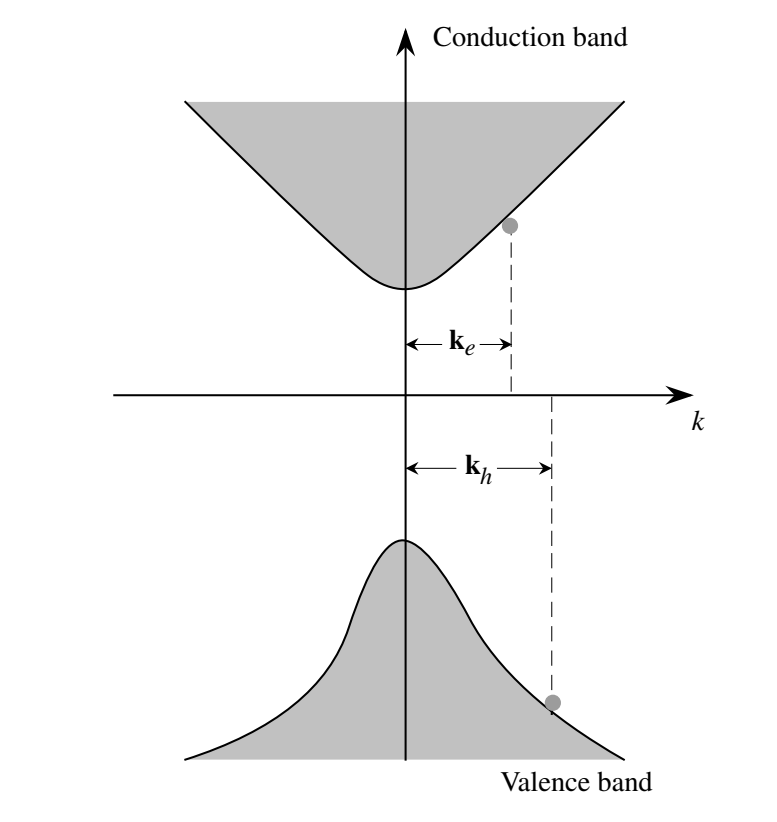
\includegraphics[width=\textwidth]{img/Exciton_Block.png}
		\\[0.5em]
		\refstepcounter{figure}
		\textbf{Figure~\thefigure.} Schematic picture of an exciton in the Bloch representation.
		\label{fig:Exciton_Block}
	\end{minipage}
\end{center}
\chapter{Paper Exam}
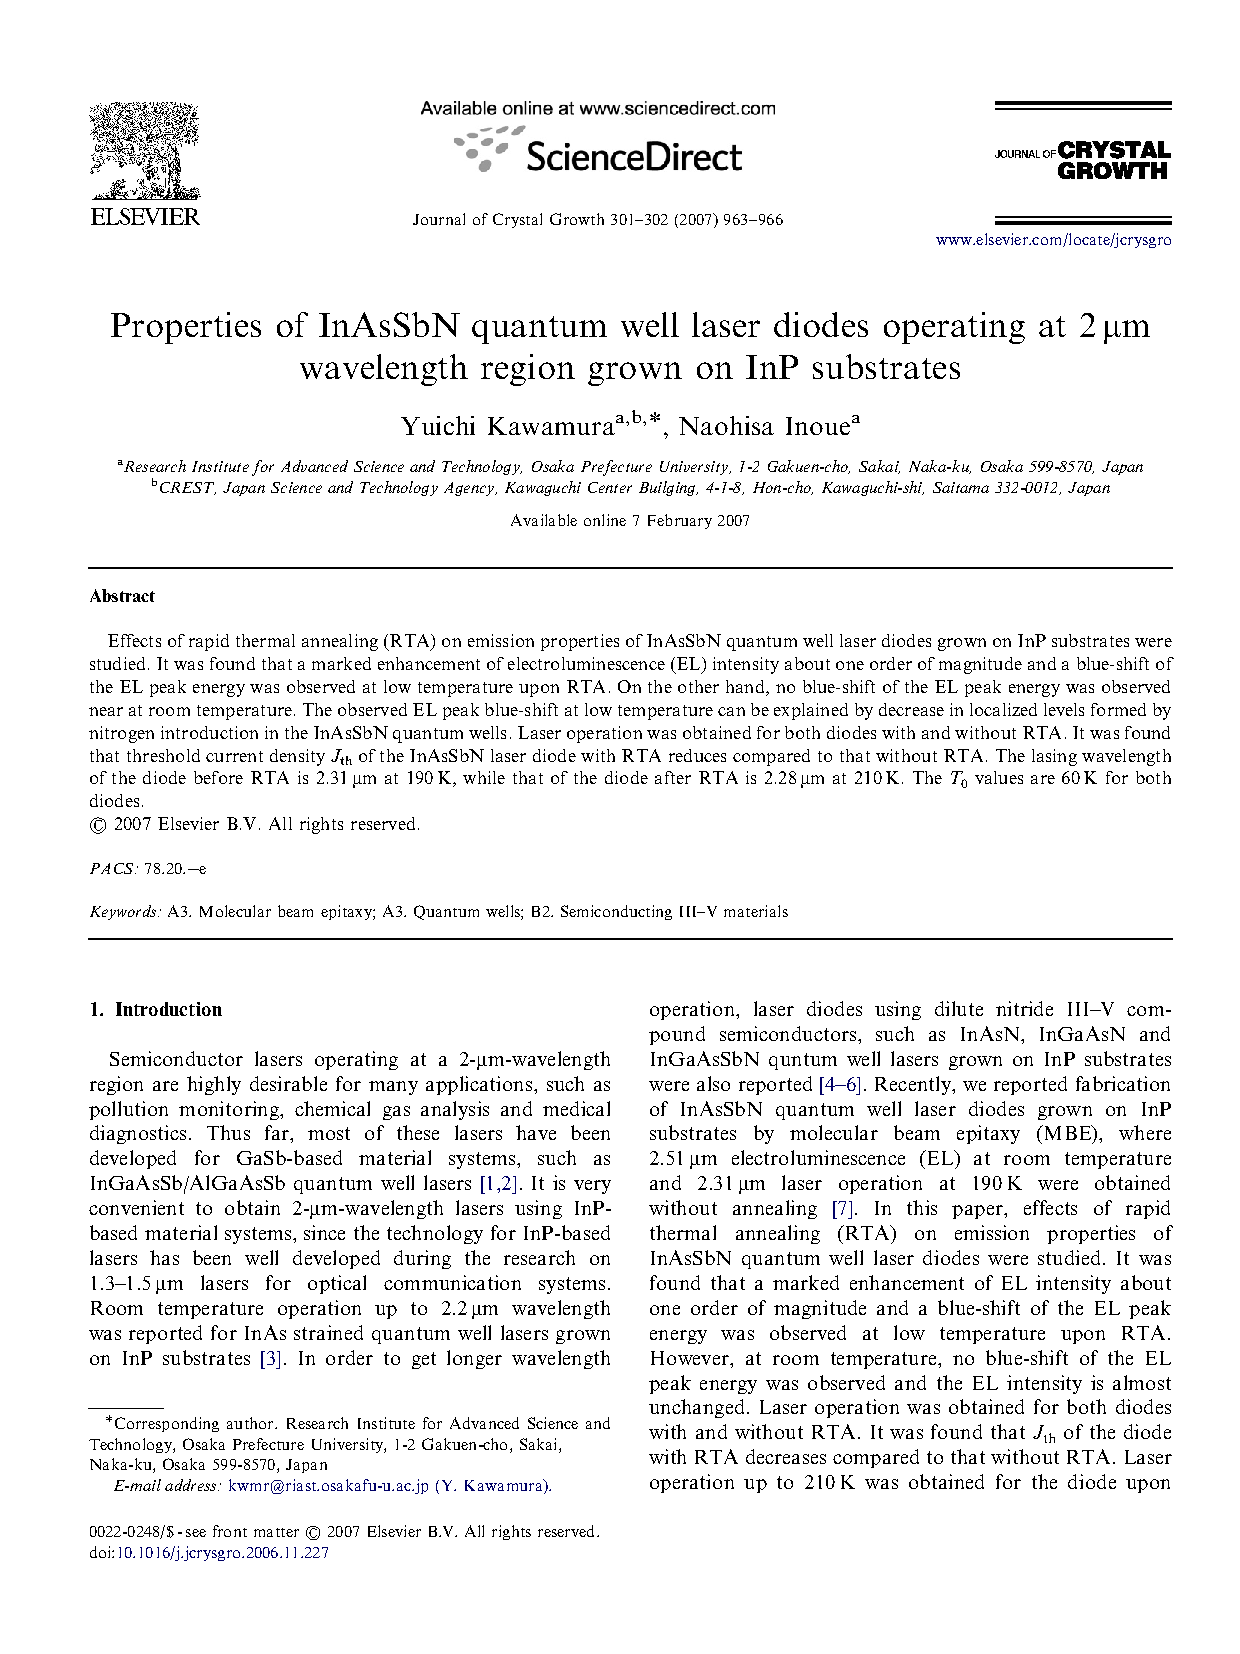
\includepdf[pages=-]{chapters/esame-annealing.pdf}

% -----------------------
% Bibliografia
% -----------------------
\cleardoublepage
\phantomsection
\addcontentsline{toc}{chapter}{Bibliografia}
\bibliographystyle{ieeetr}
\bibliography{bibliography}

\end{document}
